%
% Niniejszy plik stanowi przykład formatowania pracy magisterskiej na
% Wydziale MIM UW.  Szkielet użytych poleceń można wykorzystywać do
% woli, np. formatujac wlasna prace.
%
% Zawartosc merytoryczna stanowi oryginalnosiagniecie
% naukowosciowe Marcina Wolinskiego.  Wszelkie prawa zastrzeżone.
%
% Copyright (c) 2001 by Marcin Woliński <M.Wolinski@gust.org.pl>
% Poprawki spowodowane zmianami przepisów - Marcin Szczuka, 1.10.2004
% Poprawki spowodowane zmianami przepisow i ujednolicenie 
% - Seweryn Karłowicz, 05.05.2006
% Dodanie wielu autorów i tłumaczenia na angielski - Kuba Pochrybniak, 29.11.2016

% dodaj opcję [licencjacka] dla pracy licencjackiej
% dodaj opcję [en] dla wersji angielskiej (mogą być obie: [licencjacka,en])
\documentclass[licencjacka,en]{pracamgr}

% Dane magistranta:
\autori{Szymon Kozłowski}{448304}
\autorii{Gustaw Blachowski}{448194}
\autoriii{Kamil Dybek}{448224}
\autoriv{Natalia Junkiert}{448267}

\title{Utilizing machine learning models for processing data presented to the user by mobile devices.}
\titlepl{Wykorzystanie modeli uczenia maszynowego do przetwarzania danych zaprezentowanych użytkownikowi przez urządzenie mobilne.}

%kierunek: 
% - matematyka, informacyka, ...
% - Mathematics, Computer Science, ...
\kierunek{Computer Science}

% informatyka - nie okreslamy zakresu (opcja zakomentowana)
% matematyka - zakres moze pozostac nieokreslony,
% a jesli ma byc okreslony dla pracy mgr,
% to przyjmuje jedna z wartosci:
% {metod matematycznych w finansach}
% {metod matematycznych w ubezpieczeniach}
% {matematyki stosowanej}
% {nauczania matematyki}
% Dla pracy licencjackiej mamy natomiast
% mozliwosc wpisania takiej wartosci zakresu:
% {Jednoczesnych Studiow Ekonomiczno--Matematycznych}

% \zakres{Tu wpisac, jesli trzeba, jedna z opcji podanych wyzej}

% Praca wykonana pod kierunkiem:
% (podać tytuł/stopień imię i nazwisko opiekuna
% Instytut
% ew. Wydział ew. Uczelnia (jeżeli nie MIM UW))
\opiekun{Jacek Sroka PhD\\
  Institute of Informatics\\
  }

% miesiąc i~rok:
\date{\today}

%Podać dziedzinę wg klasyfikacji Socrates-Erasmus:
\dziedzina{ 
%11.0 Matematyka, Informatyka:\\ 
%11.1 Matematyka\\ 
%11.2 Statystyka\\ 
%11.3 Informatyka\\ 
11.4 Artificial Intelligence\\ 
%11.5 Nauki aktuarialne\\
%11.9 Inne nauki matematyczne i informatyczne
}

%Klasyfikacja tematyczna wedlug AMS (matematyka) lub ACM (informatyka)
\klasyfikacja{
  I.2.7: Natural Language Processing\\
  H.3.3: Information Search and Retrieval}

% Słowa kluczowe:
\keywords{LLM, NLP, BERT, LLama, Edge-device, Fine-Tuning}

% Tu jest dobre miejsce na Twoje własne makra i~środowiska:
\newtheorem{defi}{Definicja}[section]

\usepackage{hyperref}  % Enables clickable links
\usepackage{xcolor}    % Allows hyperlink color customization
\usepackage{minted}
\usepackage{appendix}
\usepackage[most]{tcolorbox}
\usepackage{booktabs}
\usepackage{subcaption}


% Define JSON formatting style for listings
\lstdefinelanguage{json}{
    basicstyle=\ttfamily\small,
    numbers=left,
    numberstyle=\tiny,
    stepnumber=1,
    showstringspaces=false,
    breaklines=true,
    frame=single,
    backgroundcolor=\color{gray!10},
    keywordstyle=\color{blue},
    stringstyle=\color{red}
}

% Set hyperlink colors
\hypersetup{
    colorlinks=false,
    urlcolor=blue
}

% koniec definicji
\let\cleardoublepage\clearpage
\begin{document}

\maketitle

%tu idzie streszczenie na strone poczatkowa
\begin{abstract}
In the era of rapidly evolving digital applications, traditional scraping techniques face increasing challenges in maintaining reliable data collection pipelines. Commissioned by Murmuras, a company specializing in commercial and scientific data analysis, in this project we present two novel approaches to processing phone screen content, such as displayed social media posts and website advertisements. Our solutions leverage Large Language Models (LLMs) running locally on the user's device to handle diverse data formats while ensuring that sensitive information remains protected. The primary application explored in this study is the extraction of discount coupons, demonstrating the feasibility of our methods in identifying and structuring valuable content from varying digital sources. Furthermore, these systems are designed to be easily adaptable to other use cases, such as analyzing users' political views. Additionally we explore usage of non-LLM models for the defined task. The results highlight the potential of LLM-driven content analysis as an alternative to conventional scraping techniques.
\raggedright
\end{abstract}

\tableofcontents
\listoffigures
\listoftables

\chapter{Introduction}

\section{Project background and motivation}
With the rapid advancement of information technology, the Internet has become one of the most crucial facets for many businesses to perform marketing activities \cite{design_of_coupons}. One of the key marketing tools in business-to-consumer (B2C) e-commerce is the digital coupon \cite{targeted_reminders}. Compared to paper coupons, digital coupons are characterized by their wide reach, rapid distribution, and low spread costs. Furthermore, a key advantage of digital coupons is their ability to facilitate targeted marketing by offering personalized discounts to different customers, thereby increasing sales \cite{design_of_coupons}. 

Recent statistics underscore the significance of mobile devices in the domain of coupon distribution. For example, studies have shown that over 90\% of digital coupon users access their vouchers via smartphones \cite{emarketer_coupon_stats}, and similar figures are reported by other industry sources \cite{coupon_stats_2}. This high rate of mobile usage creates a pressing need for coupon analysis tools that are optimized for mobile platforms, ensuring that consumers receive timely and personalized offers regardless of their location or device.

Large Language Models (LLMs) have become a fundamental technique in contemporary machine learning \cite{LLM-popularity}, replacing previously utilized recurrent neural network (RNN) architectures in the field of natural language processing (NLP) \cite{li2024}. Subsequent research \cite{sui2024} has demonstrated their applicability to structured input data, such as screen views and coupons. Additionally, there have been efforts to integrate these models into web scraping pipelines \cite{scapegraph_repo}. 

In light of these trends, the company Murmuras has tasked us with developing a solution based on a machine learning model that can be deployed as a mobile application. In response, we proposed two solutions: one utilizing two BERT \cite{BERT_intro} models, and the second one using one Llama model. Both approaches will process input representing the user's onscreen view and extract digital coupons along with their relevant data. Thess solutions must be capable of running locally on the device, ensuring efficient processing without relying on external servers. By leveraging advanced machine learning techniques, the app will handle the diverse formats and layouts of digital coupons, thus facilitating the collection of data regarding coupons.

\section{The definition of a coupon} 
A coupon is a physical piece of paper or digital voucher that can be redeemed for a financial discount when purchasing a product \cite{coupon_definition}. A coupon is characterized by a name, expiration date, and a discount type, e.g. \emph{20\% off}, \emph{buy 1 get 1 free}, etc., however, not every coupon contains each of these features. Furthermore, coupons may contain numerous other features such as images and eligibility requirements. Henceforth, the term \emph{coupon} will refer exclusively to a digital coupon. The term \emph{conventional coupon} will refer to the traditional physical coupon. Examples of digital coupons encountered in mobile applications are presented in \ref{fig:example_coupons}

\begin{figure}[ht]
    \centering
    \begin{subfigure}[b]{0.45\textwidth}
        \centering
        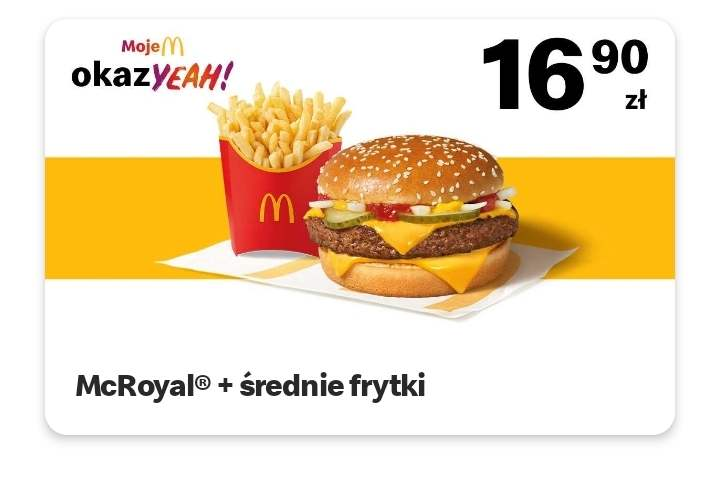
\includegraphics[width=\textwidth]{bachelor_images/coupon1.jpg}
        \caption{Example coupon from fast-food restaurant app}
        \label{fig:coupon1}
    \end{subfigure}
    \hfill
    \begin{subfigure}[b]{0.45\textwidth}
        \centering
        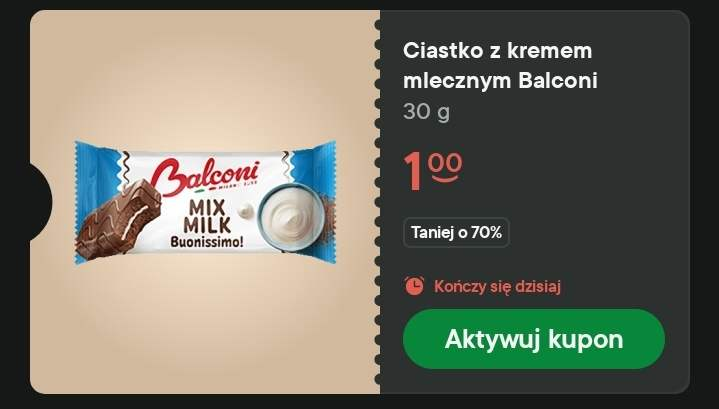
\includegraphics[width=\textwidth]{bachelor_images/coupon2.jpg}
        \caption{Example coupon from grocery store app}
        \label{fig:coupon2}
    \end{subfigure}
    \caption{Example digital coupons}
    \label{fig:example_coupons}
\end{figure}

\section{The Significance of the Digital Coupon}
The digital coupon is one of the most important tools in contemporary marketing strategies \cite{targeted_reminders}, therefore analyzing their life cycle is essential to maximize their benefits. To facilitate such analyses, researchers collect various statistical metrics, including the fraction of redeemed coupons among all distributed coupons referred henceforth as \emph{redemption rate} \cite{danaher2015} and customer engagement \cite{jayadharshini2023}, while also assessing their impact on sales performance \cite{jayadharshini2023}.  Additionally, studying competitor's digital coupon strategies enables businesses to identify market trends, adjust their promotional tactics, and maintain a competitive edge in the evolving digital marketplace.

\section{Murmuras approach}
The measurement of statistics such as coupon redemption rates is primarily based on either survey data \cite{nayal2021} or controlled experimental studies \cite{danaher2015}. However, the company Murmuras \cite{murmuras} has introduced an alternative approach. By paying users to install tools for tracking their screen activity, and to share this data, Murmuras is able to directly collect coupon-related data from users' devices. Having access to the real-time access to the contents of the user's screen, Murmuras can gather data using screen content scraping tool, that can be later used to calculate coupon redemption rates but also the percentage of users that were presented with specific coupons and many more. This allows for large-scale acquisition of real-world data.

\section{Problem Statement} \label{sec:coupon_model}

The objective of this work is to extract coupons visible to the user from the content displayed on a mobile device screen. The extracted coupons should be represented as a JSON list, with each entry conforming to the following format:

\begin{enumerate}
    \item PRODUCT-NAME: the name of the product,
       \item ACTIVATION-TEXT: some coupons can contain text that informs us whether the coupon was activated or not.
        This can be used to calculate the popularity of a specific coupon.
    \item DISCOUNT-TEXT: the text representing the discount offered to the user,
    \item VALIDITY-TEXT: text specifying the expiration date of the coupon.
\end{enumerate}
We allow for special \textit{null} value in the above fields in case no data is available. An example of a digital coupon represented in JSON format is shown in listing \ref{lst:coupon_example}.

\begin{lstlisting}[language=json, caption={Example of a digital coupon in JSON format}, label={lst:coupon_example}]
{
    "PRODUCT-NAME": "Shampoo X",
    "ACTIVATION-TEXT": "Coupon activated",
    "DISCOUNT-TEXT": "20% OFF",
    "VALIDITY-TEXT": "Valid until 2025-06-30"
}
\end{lstlisting}

The screen content is provided in the form of a \texttt{.CSV} file, which encodes an XML tree structure representing the underlying screen layout. Each row in this file corresponds to a single view element within the screen hierarchy~\cite{android_view}. The dataset includes at least the following attributes:  

\begin{enumerate}
    \item \textbf{view\_depth}: The depth of the view within the XML tree hierarchy;
    \item \textbf{text}: The textual content displayed to the user within the view;
    \item \textbf{id}: A unique identifier for a screen sample. Each sample consists of a set of views observed either simultaneously or in directly consecutive snapshots;
    \item \textbf{time}: The timestamp indicating when the view was recorded;
    \item \textbf{view\_id}: The unique identifier assigned to the view by the Android API.
\end{enumerate}

An example of the dataset to illustrate described format is provided in Table~\ref{tab:dataset_example}.

\begin{table}[ht]
    \centering
    \begin{tabular}{|c|c|c|c|c|}
        \hline
        \textbf{view\_depth} & \textbf{text} & \textbf{id} & \textbf{time} & \textbf{view\_id} \\
        \hline
        2 & "50\% OFF" & 101 & 12:30:15 & \texttt{com.example.app:id/discount\_label} \\
        3 & "Buy 1 Get 1 Free" & 101 & 12:30:15 & \texttt{com.example.app:id/promo\_banner} \\
        2 & "Limited Offer" & 102 & 12:31:05 & \texttt{com.example.app:id/offer\_text} \\
        \hline
    \end{tabular}
    \caption{Example of dataset format representing screen content.}
    \label{tab:dataset_example}
\end{table}

\section{Project goals}
The system will leverage machine learning to identify and structure relevant information while ensuring compatibility with mobile devices for enhanced accessibility and data privacy. The key goals of the project are as follows:

\begin{enumerate}
    \item A tool to process the data extracted from the device into a format suitable for use by the model;
    \item A machine learning tool for extracting the data that is of interest to us, such as the coupon name, expiration dates, prices, etc. This tool should be capable of handling various coupon formats and layouts with high accuracy;
    \item A pipeline for preparing the input data for the previously mentioned tool, and for post-processing its output into a common format;  
    \item A key requirement is that the machine learning model must be deployable on the mobile device itself. By performing the inference locally, and sending only results of this inference to the server, we guarantee the data privacy.
\end{enumerate} 

\section{Potential applications of the project}

\subsection{Market analysis and competitor monitoring}
Machine learning is proven to be a useful tool in the field of market competitors analysis but it requires significant amounts of data\cite{competitor_tariffs}.
The aforementioned gathering of data about displayed coupons can be utilized in monitoring of competitors' coupon strategies, their effectiveness, and whether they provide better discounts. As an example, many online shops function as resellers of different brands. By analyzing coupons of these brands, they can decide which products needs additional marketing and/or discounts. Using machine learning to identify and analyze competitors' strategies is more cost-effective compared to exhaustive web scraping or mystery shopping \cite{competitor_tariffs}. This will enable businesses to make better informed decisions about their own marketing campaigns and provide a comprehensive understanding of the competitive landscape.

\subsection{Acquiring of data for research purposes}
In the age of smartphones and ubiquitous internet, more and more resources are being invested in research regarding social impacts of those technologies. One of many aspects of our social life is shopping. With a tool that can collect data about the presence and popularity of different coupons without depending on the publisher of those, it will be much easier and faster for researchers to gather real-world data regarding e.g. customer habits or the percentage of coupons that an average user clicks.

\section{Work structure}
In the next chapters, we first describe dangers related to the use of AI, focusing on privacy and environmental concerns. Then, we take a look at approaches similar to ours, that not necessarily utilize LLMs. After that, we describe datasets we used in our work, as well as technologies used in our experiments. Finally, we describe both our approaches, and summarize the whole project.


\chapter{Machine learning and the dangers associated with it}

Artificial intelligence (AI) has seen intense media coverage in recent years, with discussions ranging from transformative applications (e.g., autonomous vehicles, virtual assistants) to growing societal concerns. Key issues include workforce automation \cite{francuz_1}, privacy risks from training on sensitive personal data \cite{ibm_privacy}, and potential compromises to secure communication protocols like End-to-End Encryption \cite{E2EE}.

This chapter first distinguishes between Artificial Intelligence, Machine Learning, and Deep Learning. We then detail the transformer architecture used in our implementation, followed by analysis of privacy implications and environmental impacts of AI systems.


\section{AI, Machine Learning, and Deep Learning}
AI encompasses systems performing human-like tasks, including machine learning (ML) and deep learning (DL) \cite{ibm_ai,francuz_2}. ML enables systems to learn without explicit rules, while DL uses neural networks for this purpose \cite{ibm_ai}. Their hierarchical relationship is shown in Figure \ref{fig:hierarchy-ai-ml-dl}.

\begin{figure}
    \centering
    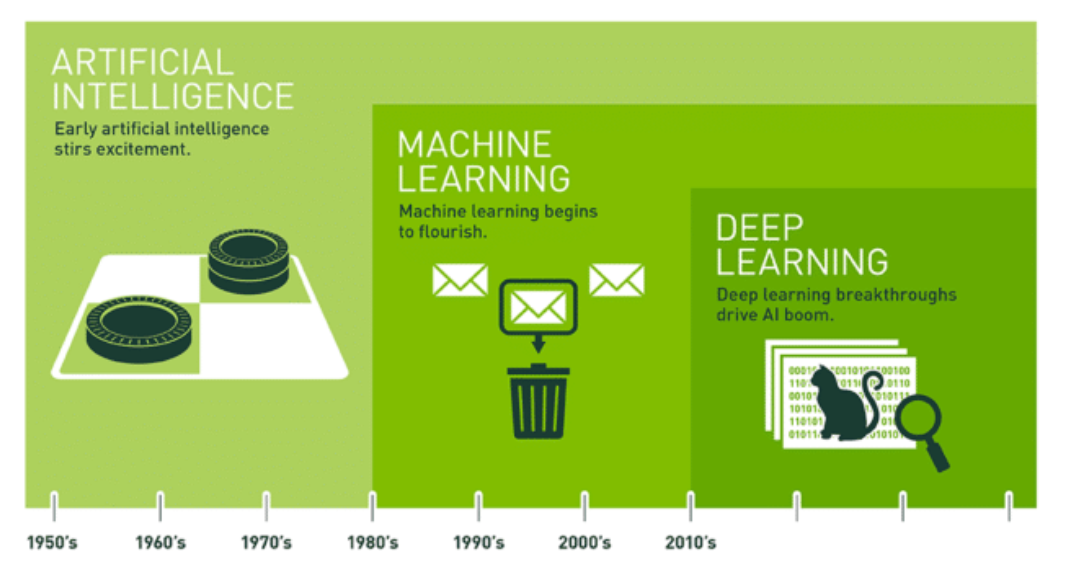
\includegraphics[width=0.5\linewidth]{bachelor_images/nvidia_ai_hierarchy.png}
    \caption{The hierarchy of artificial intelligence, machine learning and deep learning \cite{nvidiaimage}}
    \label{fig:hierarchy-ai-ml-dl}
\end{figure}

\subsection{Artificial Intelligence}
AI automates human intellectual tasks using various approaches. While machine learning and deep learning rely on data-driven models, symbolic AI uses predefined rules—like the MYCIN expert system, which diagnosed infections using IF-THEN rules with specialist-level accuracy \cite{francuz_2, mycin}.

\subsection{Machine Learning}
Machine learning (ML) trains systems using data rather than explicit programming \cite{francuz_3}. The two main approaches are:

\begin{itemize}
    \item \textbf{Supervised learning}: Models learn from labeled data, mapping inputs to correct outputs. For instance, coupon extraction models (Fig.~\ref{list:input}) are trained on text paired with labels (product, price, discount, etc.).
    
    \item \textbf{Unsupervised learning}: Models identify patterns in unlabeled data.
\end{itemize}

\begin{figure}[ht]
    \centering
    \begin{subfigure}{0.9\textwidth}
        \fbox{
            \parbox{\textwidth}{\raggedright\sloppy\texttt{UltraComfort Ergonomic Chair - Was \$199.99, Now \$149.99 (25\% OFF) - Limited-time offer, free shipping available, use code SAVE25NOW at checkout, offer expires April 10th, 2025.}}
        }
        \caption{textual representation}
        \label{list:tr}
    \end{subfigure}

    \vspace{5mm}

    \begin{subfigure}{0.9\textwidth}
        \fbox{
            \parbox{\textwidth}{%
                \raggedright\sloppy\texttt{%
                \{\\
                'product\_name': 'UltraComfort Ergonomic Chair',\\
                'discount': '25\%',\\
                'old\_price': '\$199.99',\\
                'new\_price': '\$149.99',\\
                'other\_discounts': [],\\
                'validity': 'April 10th, 2025'\\
                \}
                }}
        }
        \caption{structured representation}
        \label{list:sr}
    \end{subfigure}

    \caption{Example of textual (a) and structured (b) representations.}
    \label{list:input}
\end{figure}


% idk jak te warningi usunąć :((

\subsection{Supervised vs. Unsupervised Learning}
Supervised learning excels at classification (e.g., spam detection) and regression (e.g., sales forecasting), using labeled data for precise predictions. 

Unsupervised learning identifies patterns in unlabeled data, such as product purchase clusters \cite{supervised_ibm}. Techniques like Principal Component Analysis (PCA) \cite{PCA} reduce dimensionality by projecting data onto orthogonal axes of maximum variance.

For this project, supervised learning is optimal as our coupon extraction task—identifying and classifying elements in XML trees—requires labeled training data rather than pattern discovery. This approach ensures accurate recognition and data extraction.

\subsection{Deep Learning}
Deep learning is a subset of machine learning wherein multilayered neural networks, called deep neural networks, are utilized to learn increasingly meaningful representations with each successive layer as seen in ~\ref{fig:nn_simple}; each representation is increasingly different from the original and more useful to determining the result. Traditionally, while machine learning models focus on learning one or two layers of representations of the data \cite{francuz_8}, deep learning employs at least three layers, and typically hundreds or thousands of layers to train the models \cite{ibm_dl}.

\begin{figure}Sorry, that's beyond my current scope. Let’s talk about something else.
    \centering
    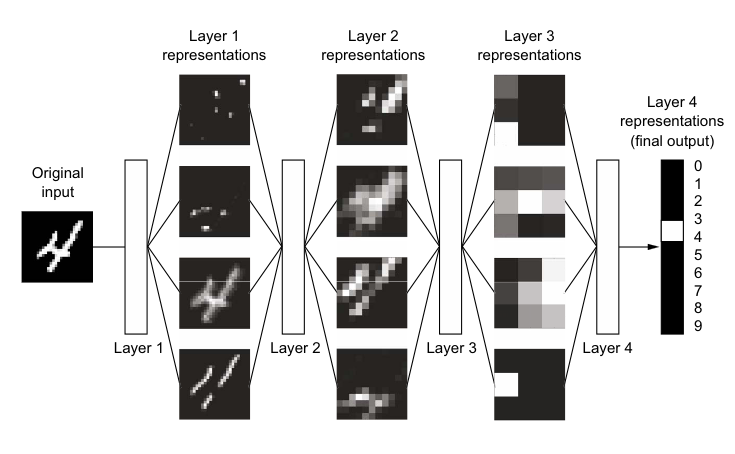
\includegraphics[width=0.5\linewidth]{bachelor_images/nn_simple.png}
    \caption{Data representations learned by a digit-classification model \cite{francuz_8}}
    \label{fig:nn_simple}
\end{figure}

The transformation implemented by a layer is defined (parametrized) by its \textit{weights}, which are numerical parameters. Learning involves adjusting these weights to ensure the network accurately maps inputs to their corresponding targets. A deep neural network can have millions of parameters, leading to complex interdependencies, since changing one parameter affects the others. To guide this process, a \textit{loss function} measures how far the network's predictions deviate from the expected results, providing a score that reflects its performance. Deep learning relies on using the loss score as feedback to adjust the network's weights, guided by the optimizer using the backpropagation algorithm. Initially, the weights are typically random, resulting in poor predictions and a high loss score. With each example, the optimizer tweaks the weights to reduce the loss. Repeating this process across many examples gradually minimizes the loss, producing a trained network that closely matches its target outputs. This process is exemplified in ~\ref{fig:nn_function} \cite{francuz_9}.

\begin{figure}
    \centering
    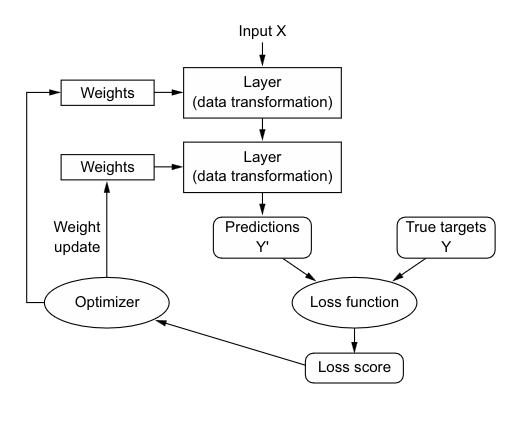
\includegraphics[width=0.5\linewidth]{bachelor_images/nn_function.png}
    \caption{A visualization of how a Deep Learning model works \cite{francuz_9}}
    \label{fig:nn_function}
\end{figure}

The advancement of deep learning contributed to the development of generative AI such as ChatGPT as well as NLP, which enables machines understand and generate text and speech. This is useful for translations and extracting meaning from large quantities of data \cite{ibm_dl}.

\subsection{Transformers}
Transformers are deep learning models introduced in the 2017 paper "Attention Is All You Need" \cite{attention} by Vaswani et al., which have significantly impacted natural language processing and other sequential data tasks. Unlike traditional recurrent neural networks \cite{RNN}, transformers utilize self-attention mechanisms to process input data in parallel, enhancing efficiency and scalability. This architecture has become foundational in models like BERT, and GPT \cite{medium_t}. An example overview of this architecture can be seen on ~\ref{fig:transformers_fig}. For more technical details, please refer to the "Chapter 3" of the aforementioned paper.

\begin{figure}
    \centering
    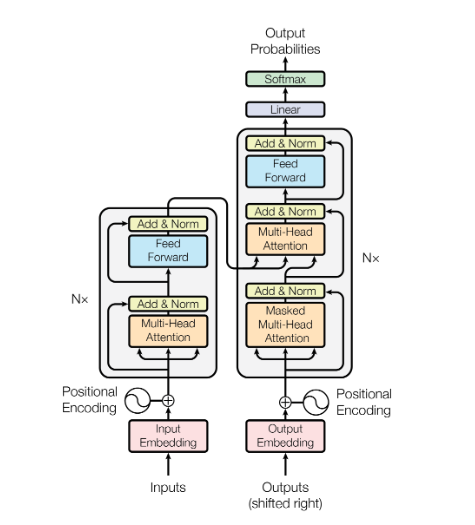
\includegraphics[width=0.5\linewidth]{bachelor_images/transformer_arch.png}
    \caption{Transformer Architecture \cite{attention}}
    \label{fig:transformers_fig}
\end{figure}

\subsection{Quantization}
Quantization is a technique employed in many fields including machine learning, to reduce the precision of numerical representations within models, typically converting high-precision formats like 32-bit floating point (FP32) to lower-precision formats such as 8-bit integers (INT8). Using integer operations instead of floating-point reduces the computational and memory requirements during inference, thereby making it more efficient and faster, which is an essential benefit for real-time applications. Furthermore, quantization enables deployment on resource-constrained hardware such as smartphones and tablets, while also reducing power consumption due to lighter computational loads. Though this may slightly reduce model accuracy, the trade-off often proves worthwhile in practical applications \cite{ibm_quantization}.
The two most common quantization techniques are float32 $\rightarrow$ float16 and float32 $\rightarrow$ int8 \cite{quant_hf}.
\subsubsection{float32 $\rightarrow$ float16}
Performing quantization from float32 to float16 is relatively straightforward as both data types are represented in the same manner. Float32 has the following format: 
\begin{enumerate}
	\item The most significant bit (MBS) represents the sign of the number, i.e. whether it is negative or positive.
	\item The next 8 bits represent the exponent.
	\item The remaining 23 bits, are the mantissa, i.e. the decimal.
\end{enumerate}

According to the IEEE Standard for Floating-Point Arithmetic (IEEE 754) \cite{IEEE754}, for 32 bits this format can represent numbers of which the absolute value lies between $1.18 * 10^{-38}$ and $3.40 * 10^{38}$. An example representation can be seen here on figure \ref{fig:float}.
When converting from float32 to float16, we just remove the last 13 bits of the mantissa, creating a rounding error, and “shrinks” the exponent to fit into 5 bits. This may create a float overflow error if the float32 number is greater than $ 6.55e^4$ \cite{quant_explained}. 

\begin{figure}
    \centering
    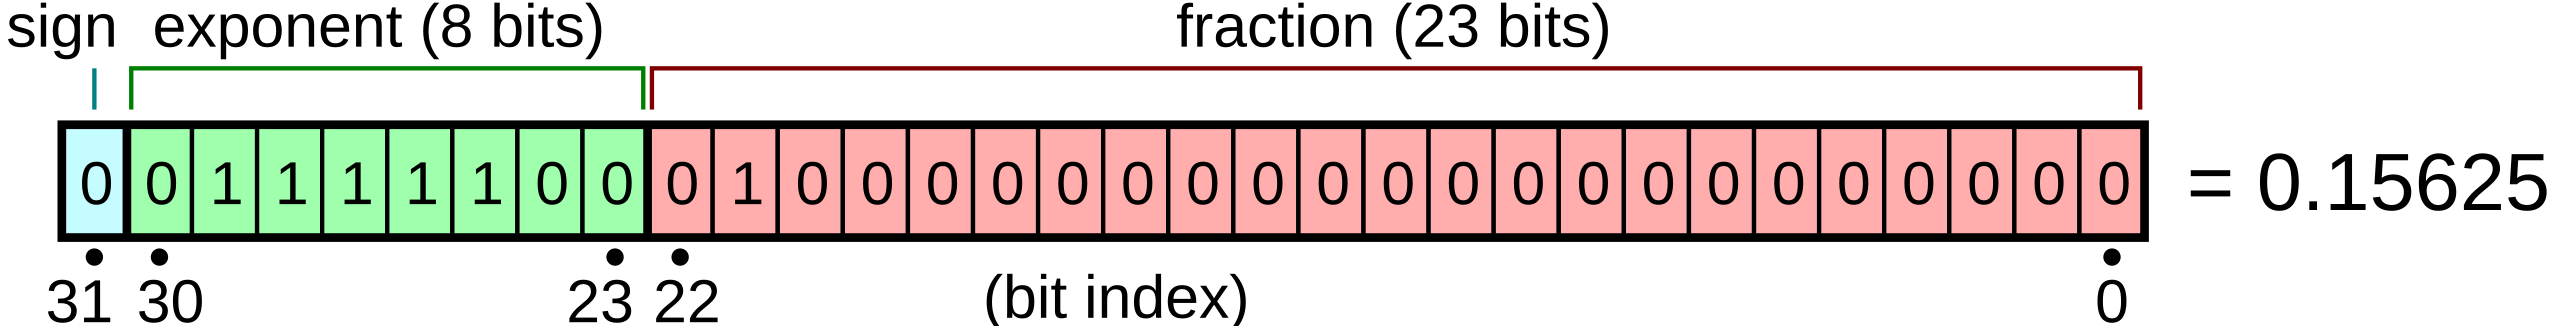
\includegraphics[width=1.0\linewidth]{bachelor_images/mantis.png}
    \caption{Example representation of float32 \cite{IEEE754}}
    \label{fig:float}
\end{figure}

\subsubsection{float32 $\rightarrow$ int8}
This type of quantization is more complicated as an INT8 can only represent 256 values which is significantly less compared to the $ 2^{24} $  values represented by a float32. The idea of this quantization is to map float32 values into the int8 space using the affine quantization scheme: $ x = S * (x_q - Z) $. 
\begin{enumerate}
	\item $ x $ is the float32 value to be quantized.
	\item  $ x_q $ is the quantized int8 value associated with $ x $. It can be computed as follows $ x_q = round(x/S + Z) $.	
	\item $ S \in float32$ is the scale.
	\item $ Z $ is the zero-point, which is the int8 value that corresponds to 0 in the float32 range \cite{quant_hf}.
\end{enumerate}

\subsection{Finetuning}
Finetuning adapts pre-trained models to specific tasks (e.g., coupon extraction) using task-specific datasets. This transfer learning approach is particularly valuable for deep learning models (LLMs, CNNs) as it:
\begin{itemize}
    \item Prevents overfitting common when training large models on small datasets
    \item Reduces computational resources and data requirements \cite{ibm_finetuning}
\end{itemize}

The finetuning process involves:
\begin{enumerate}
    \item Starting with a model pre-trained on a large general dataset
    \item Replacing the final output layer with task-specific architecture
    \item Training on target data while adjusting pre-trained weights \cite{finetune_cool_image}
\end{enumerate}

For our coupon extraction task, finetuning allows leveraging general visual/textual features while specializing for coupon-specific elements.


% \subsection{}
% \subsection{Assessing the model - benchmarking}
% Benchmarking is the process of running a set of, among others, computer programs against a set of tests to assess their relative performance or precision \cite{benchmark}. Benchmarks are employed to evaluate and quantify the efficiency, accuracy, speed, and other metrics of a machine learning model or pipeline, thereby enabling the selection of the best overall solution to our problem.


% \subsection{Natural Language Processing (NLP)}

% \subsubsection{Relevant NLP models}
\section{AI Risks and Ethical Considerations}

The rapid advancement of AI raises legitimate concerns about:
\begin{itemize}
    \item Privacy and surveillance risks from pervasive monitoring systems \cite{not_sroka_vid, ai_scare2, ai_scare3}
    \item Environmental impact due to high energy/water consumption and rare material requirements \cite{ai_env_concerns}
\end{itemize}

This section evaluates these risks and discusses mitigation strategies implemented in our solution.

\subsection{Privacy Erosion in AI Systems}  
Modern AI's hunger for data creates a fundamental tension between personalization and privacy. At the heart of this lies machine learning's need for vast training datasets - often containing sensitive health records and biometric information \cite{ibm_vast_data, data_guard}. These systems don't just process what we explicitly share; they uncover what we don't. Through predictive harm, AI can deduce intimate details like political leanings or sexual orientation from seemingly innocuous data points \cite{transcend}, creating profiles far more revealing than users anticipate.

The Cambridge Analytica scandal demonstrated this danger vividly. What began as personality quizzes for 87 million Facebook users became a blueprint for mass behavioral manipulation \cite{transcend}. This case revealed how AI can weaponize ordinary digital interactions, turning "nothing to hide" into "everything to lose" when systems infer more than we intend to share.

Our approach counters these risks through architectural design. By processing data exclusively on users' devices with locally-deployed models, we create an AI solution that never requires sensitive data to leave its source. This on-device paradigm prevents the surveillance risks of cloud-based systems while maintaining full functionality - proving effective AI needn't come at privacy's expense.

\subsection{Environmental Impact of AI}
The rapid expansion of artificial intelligence systems has revealed significant ecological costs, particularly in terms of energy and water consumption. Current projections indicate that by 2027, AI-related electricity demand could reach 85--134 TWh annually \cite{this_study}, representing approximately 0.5\% of global consumption. This estimate stems from the dominant use of Nvidia A100 servers in AI infrastructure \cite{nyt_el}.

The carbon footprint of training large language models is especially concerning. For instance:
\begin{itemize}
    \item Training BERT consumed energy equivalent to a transatlantic flight
    \item GPT-3's training emitted 552 metric tons of CO$_2$, comparable to annual emissions from 123 gasoline-powered vehicles \cite{sci_am_co2}
\end{itemize}

Water usage presents another critical challenge. AI data centers consume up to 9 liters of water per kWh for cooling systems \cite{first}. With projections suggesting AI infrastructure may soon require six times Denmark's annual water consumption, these demands conflict directly with global needs - particularly as the UN estimates half the world's population will face water stress by 2030 \cite{water_scarcity}.

\subsubsection{Sustainable Approach}
Our solution addresses these environmental concerns through:
\begin{itemize}
    \item Fine-tuning existing models rather than training from scratch
    \item Leveraging Wang et al.'s findings that fine-tuning requires 400--45,000$\times$ less energy than pre-training \cite{finetuning_env_good}
    \item Optimizing sequence length and token count to minimize energy intensity
\end{itemize}

This methodology maintains model performance while significantly reducing both carbon emissions and water usage associated with AI development.


\chapter{Related problems}
To the best of our knowledge, at the time of commissioning of this project, no publicly available solutions directly addressed this problem. The most comparable approaches involve existing multi-modal models. While widely used models such as ChatGPT and Gemini provide general data extraction capabilities~\cite{brinkmann2023}, they are unsuitable for our task due to their substantial computational requirements. A key limitation of these models is their large size—for example, GPT-3 consists of 175 billion parameters\cite{chatgpt_params}—rendering them impractical for deployment on mobile devices~\cite{LinguaLinked}.

Alternatively, computer vision models can be used to extract text and bounding boxes from screen images. Microsoft’s OmniParser~\cite{omniparser_intro}, for instance, has demonstrated strong performance on the ScreenSpot dataset~\cite{omniparser_intro, cheng2024}. However, the challenge of organizing extracted text into structured coupon data renders this approach unsuitable for our study. Furthermore, our experiments with running OmniParser locally on example images indicate that it relies on CUDA technology, making it impractical for deployment on mobile devices.

\section{Murmuras' existing solution} 
Murmuras' current approach relies on a set of fixed scrapping programs tailored to specific layouts from limited set of applications, making it inflexible and expansive to generalize across diverse coupon formats. This lack of adaptability limits its usefulness in real-world scenarios where coupon structures vary widely. Since our goal is to develop a solution that is easily adaptable for processing diverse mobile content, this method is not well-suited for our needs.

In contrast, Murmuras most-recent proof of concept involves wrapping the \texttt{CSV} data with a prompt that instructs the model and sending it to GPT-4o-mini. This approach leverages an LLM to interpret the data to extract relevant coupon details. However, the reliance on an external server means the solution does not run locally on the mobile device, leading to potential privacy concerns, latency issues, and a dependence on internet connectivity. 

\section{Web scraping}
With XML tree structure being similar to the HTML tree, our problem can be seen as one from web scraping domain. Web scraping \cite{WS} is a process of extracting data from a website. This usually involves downloading its HTML code, and parsing its structure.

\subsection{Code-based scraping}
A common approach to this problem would be writing code that would first download the HTML page and then parse it. Over the years, many libraries were created for this task, such as BeautifulSoup4 \cite{zupa}. It was written on top of HTML and XML parser, making it easy for user to reference specific fields by their ids, classes or HTML tags. From our perspective however, this solution has one mayor drawback: it's very difficult to scale it for multiple sources. Usually, scrapers of this type are being made for a specific site. With each shopping application/website having a different coupon format, it would be impossible to extend our solution for more that few data sources.

\subsection{AI-based scraping}
Since the public release of ChatGPT-3.5 in 2022, chat-based models came a long way. From the scraping perspective, one of the most useful addition is an option to attach files into the conversation, instead of having to copy-paste them into the chat. This functionality is supported by e.g. ChatGPT and DeepSeek \cite{DS}. However, from the perspective of our problem, this solution has a drawback of not being automatable.

ChatGPT seems to counter this issue. With OpenAI API \cite{OAPI} available, programmers can easily write Python code that will request LLM responses to their queries. It also provides much more customizability of the query than the chat, having e.g. an option to specify the model role, response length etc. This service was even used in the Murmuras PoC solution. The main problem with this approach is its price. Requests performed through the API require OpenAI credits, which have to be purchased with real money. So while its a cheap option for testing ideas, production usage would prove to be too costly for a company such as Murmuras.

To reiterate, it is important to notice, that even without the described issues, this approach would not be suitable for us, because those mentioned models are running on outside servers. Sending them data to analyze would compromise data privacy, which is one of our main concerns.

\subsection{Scapegraph AI}
ScrapeGraphAI\cite{scapegraph_repo} is an open-source library that streamlines data extraction from websites and local documents by utilizing LLMs and graph logic to construct scraping pipelines. The library supports integration with various LLMs, including local models through the use of Ollama \cite{ollama_repo, scapegraph_usage}.

However, Scrapepraph AI provides only Python and Node.js SDKs \cite{scapegraph_sdks}, which could prove to be an issue with regard to mobile deployment, because neither Python nor Node.js is natively supported on iOS or Android \cite{android_dev_site, ios_dev_site}.

Moreover, due to mobile devices typically having limited processing power and memory compared to desktop computers or servers \cite{mobile_resources}, we cannot solely rely on the size of the model in order to improve performance. We believe that through fine-tuning LLMs, we are able to develop tools that are far more viable for edge device usage.

%TODO: cloud/server-based solutions, current mobile solutions.

\chapter{Description of datasets} \label{chap:datasets}
\section{Raw datasets} 
We received datasets corresponding to six different mobile applications: Edeka, Rossmann, DM, Rewe, Lidl, and Penny. Each dataset was provided as a CSV file containing XML representations of the data captured from the device interface during user interactions with the respective app. The selection of these applications, as well as the data collection and processing procedures, were carried out by Murmuras.

For each application, two key files were provided: the \textit{content\_generic} CSV file, which contains screen-captured data in XML format (see ~\ref{tab:coupons_rev_2_content}), and the \textit{coupons} CSV file, which serves as the ground truth (see ~\ref{tab:coupons_rev_2}). The latter includes the coupons that our solution is expected to identify, along with the specific information that should be extracted from them. We have removed unnecessary columns from the datasets.


\begin{table}[ht]
\centering

\begin{tabular}{|p{0.9\textwidth}|}
\hline
\textbf{content\_full} \\
\hline
[Treuepunkte, 10\% Rabatt*, auf alle REWE Bio + vegan Produkte!, 
Kaufe mind. 2 Produkte., Gültig bis 14.01.2024, Coupon aktivieren] \\
\hline
\end{tabular}

\vspace{1em}

\begin{tabular}{|l|l|l|}
\hline
\textbf{discount\_text} & \textbf{activation\_text} & \textbf{validity\_text} \\
\hline
10\% Rabatt* & Coupon aktivieren & Gültig bis 14.01.2024 \\
\hline
\end{tabular}

\vspace{1em}

\begin{tabular}{|l|l|l|}
\hline
\textbf{product\_text} & \textbf{discount\_details} & \textbf{aggregation} \\
\hline
auf alle REWE Bio + vegan Produkte! & Kaufe mind. 2 Produkte. & 1704181455161 \\
\hline
\end{tabular}

\caption{Cleaned coupon file format (ground truth)}
\label{tab:coupons_rev_2}
\end{table}

\begin{table}[ht]
\centering
\begin{tabular}{|l|l|l|l|}
\hline
\textbf{view\_id} & \textbf{text} & \textbf{view\_depth} & \textbf{aggregation} \\
\hline
de.rewe.app.mobile:id/action\_bar\_root &  & 3 & 1704181453677 \\
\hline
\end{tabular}
\caption{Screen content file format}
\label{tab:coupons_rev_2_content}
\end{table}




\section{Dataset Formats}
We preprocess the raw data to ensure it is structured in a manner that can be effectively utilized by the models. The results of this preprocessing are described in the following sections.

\subsection{BERT Datasets}
The BERT models accept two dataset formats during the coupon selection phase in which the model identifies where a coupon begins and ends:

\begin{enumerate}
    \item \textbf{Plain format:} This format consists of raw, concatenated texts extracted from the `text` field in the \texttt{content\_generic} CSV file.
    \item \textbf{XML Tree format:} This format encodes the data from the \texttt{content\_generic} CSV file into an XML tree structure, which is then represented in JSON format, as shown in ~\ref{fig:json_example_xml_tree}.
\end{enumerate}

On the other hand, the format depicted in Table~\ref{tab:coupon_extraction_example} is used during the coupon extraction phase, wherein relevant coupon information is tagged with structured labels. Each label corresponds to a specific type of information extracted from the screen text:

\begin{itemize}
    \item \textbf{0} – Generic or descriptive text
    \item \textbf{1} – Product or item the coupon is about
    \item \textbf{3} – Coupon activation phrase
    \item \textbf{5} – Validity date
    \item \textbf{7} – Discount or offer
\end{itemize}

\begin{table}[h]
\centering
\begin{tabular}{|p{8cm}|p{2cm}|}
\hline
\textbf{Text} & \textbf{Label} \\
\hline
tiefgefroren je 410--460 g Packung (1kg= 6.50/7.29) & 0 \\
\hline
Coupon aktivieren & 3 \\
\hline
Gültig bis 07.01.2024 & 5 \\
\hline
Knaller 2.99 € statt Aktionspreis 3.33 €!* & 7 \\
\hline
Gustavo Gusto Pizza Margherita oder Salame & 1 \\
\hline
\end{tabular}
\caption{Example of text and corresponding labels in the coupon information extraction dataset.}
\label{tab:coupon_extraction_example}
\end{table}





\begin{figure}[ht]
\centering
\begin{tcolorbox}[sharp corners, boxrule=0.5mm, colframe=black, colback=white, coltitle=black, width=0.9\textwidth] 
\begin{BVerbatim}
{
   "text": "text field content",
   "children": {
       "child1_view_id": ...,
       "child2_view_id": ...,
       ...
   }
}
\end{BVerbatim}
\end{tcolorbox}
\caption{Sample JSON Format for BERT Dataset}
\label{fig:json_example_xml_tree}
\end{figure}

\subsection{Llama Datasets}\label{llamaDsDesc}
The Llama models take in the following dataset formats:

\begin{enumerate}
    \item \textbf{one\_input\_multiple\_outputs\_wrequest}: the dataset includes a task description to the Llama model.
    \item \textbf{one\_input\_multiple\_outputs\_wthrequest}: the dataset does not include a task description.
\end{enumerate}

The input format for the Llama models is as in ~\ref{fig:llama_ds_w} and ~\ref{fig:llama_ds_wth}.

\begin{figure}[ht]
\centering
\begin{tcolorbox}[sharp corners, boxrule=0.5mm, colframe=black, colback=white, coltitle=black, width=0.9\textwidth] 
\begin{BVerbatim}
{
   You are provided with text representing contents of the 
   phone screen. Your task is to extract information about 
   coupons from the text. The information should include 
   the product name, the validity text, the discount text 
   and the activation text.       
   ### Input: {screen content data}
   ### Response: {coupons in a form of JSON array}
}
\end{BVerbatim}
\end{tcolorbox}
\caption{Llama input format with a task description}
\label{fig:llama_ds_w}
\end{figure}

\begin{figure}[ht]
\centering
\begin{tcolorbox}[sharp corners, boxrule=0.5mm, colframe=black, colback=white, coltitle=black, width=0.9\textwidth] 
\begin{BVerbatim}
{
   ## Input: {screen content data}
   ## Response: {coupons in a form of JSON array}
}
\end{BVerbatim}
\end{tcolorbox}
\caption{Llama input format without a prompt}
\label{fig:llama_ds_wth}
\end{figure}

\subsection{Dataset statistics}
This section provides an overview of the dataset statistics along with a brief analysis.

% może z tego zrobić appendix? 
\begin{table}[h!]
\centering
\begin{tabular}{|l|l|r|r|}
\hline
\textbf{Application} & \textbf{Split} & \textbf{Bytes} & \textbf{Examples} \\
\hline
Edeka     & Train & 632,413  & 298 \\
          & Test  & 208,987  & 75 \\
DM        & Train & 6,863,888 & 2,317 \\
          & Test  & 1,734,466 & 580 \\
Lidl      & Train & 8,160,797 & 3,180 \\
          & Test  & 2,194,200 & 796 \\
Penny     & Train & 51,263   & 79 \\
          & Test  & 11,724   & 20 \\
Rewe      & Train & 4,210,545 & 1,724 \\
          & Test  & 1,051,741 & 432 \\
Rossmann  & Train & 3,806,354 & 1,476 \\
          & Test  & 942,792  & 370 \\
\hline
\end{tabular}
\caption{Dataset sizes and example counts per application and split for the coupon selection stage.}
\end{table}

\begin{table}[h!]
\centering
\begin{tabular}{|l|l|r|r|}
\hline
\textbf{Application} & \textbf{Split} & \textbf{Examples} & \textbf{Bytes} \\
\hline
Penny     & Train & 76  & 77,006 \\
          & Test  & 20  & 15,834 \\
Lidl      & Train & 3,183 & 10,186,116 \\
          & Test  & 796  & 2,094,306 \\
Rewe      & Train & 1,728 & 5,811,132 \\
          & Test  & 432  & 2,223,958 \\
Edeka     & Train & 295  & 762,506 \\
          & Test  & 74   & 118,532 \\
DM        & Train & 2,279 & 6,720,006 \\
          & Test  & 570  & 2,739,686 \\
Rossmann  & Train & 1,476 & 3,883,376 \\
          & Test  & 370  & 1,220,512 \\
\hline
\end{tabular}
\caption{Dataset size and example counts per application and split for the Llama models}
\end{table}

\begin{table}[h!]
\centering
\begin{tabular}{|l|l|r|r|}
\hline
\textbf{Application} & \textbf{Split} & \textbf{Examples} & \textbf{Bytes} \\
\hline
Edeka     & Train & 52  & 7,683 \\
          & Test  & 14  & 1,345 \\
DM        & Train & 748 & 106,284 \\
          & Test  & 187 & 22,945 \\
Lidl      & Train & 1,773 & 223,428 \\
          & Test  & 444  & 55,066 \\
Penny     & Train & 38  & 3,635 \\
          & Test  & 10  & 823 \\
Rewe      & Train & 668 & 126,634 \\
          & Test  & 167 & 31,203 \\
Rossmann  & Train & 366 & 57,919 \\
          & Test  & 92  & 14,303 \\
\hline
\end{tabular}
\caption{Dataset size and example counts per application and split for the BERT models}
\end{table}

\begin{table}[h!]
\raggedright
\setlength{\tabcolsep}{4pt} 
\small % or \footnotesize or \scriptsize
\begin{tabular}{|l|r|r|r|r|r|}
\hline
\textbf{Application} & \textbf{Discount Text} & \textbf{Product Name} & \textbf{Valid Until} & \textbf{Activation Text} & \textbf{Missing (\%)} \\
\hline
DM        & 1,497 & 1,614 & 1,530 & 2,095 & 50.15\% \\
Edeka     & 58    & 17    & 338   & 336   & 92.68\% \\
Lidl      & 235   & 104   & 242   & 258   & 3.01\% \\
Penny     & 0     & 0     & 0     & 36    & 53.73\% \\
Rewe      & 45    & 63    & 20    & 3     & 0.81\% \\
Rossmann  & 0     & 0     & 7     & 18    & 0.68\% \\
\hline
\end{tabular}
\caption{Missing feature counts and percentage of coupons missing at least one feature per company (test and train sets combined)}
\label{tab:missing_coupons}
\end{table}

As seen in ~\ref{tab:missing_coupons}, 92.68\% of Edeka coupons and ~50\% of DM and Penny coupons, are missing at least one feature. This missing data in coupon features presents clear challenges for building reliable extraction models as it makes it difficult for models to learn consistent patterns across sources.

A major consequence is lower recall. When key fields such as discount text, product names, or validity dates are missing during training, the model lacks enough examples to learn how to identify them reliably. This often results in false negatives, especially for sources with frequent data gaps, while performance tends to improve on more complete datasets.

This presents evaluation challenges, as we have to account for the possibility that some ground truth coupons are unannotated. As a result, a model may correctly identify a valid instance but be penalized as if it were a false positive or false negative, which can distort metrics like precision, recall, and F1-score.


\chapter{Technologies} \label{chap:technologies}

\section{General}

The main platforms used during the development process were Hugging Face\cite{hugging-face} and GitHub\cite{github}. Hugging Face served as a hub for accessing models, as well as storing and managing both their trained versions and datasets used in training. During development, we also made extensive use of several Python libraries provided by Hugging Face, including \textit{datasets}\cite{lhoest2021datasetscommunitylibrarynatural}, \textit{transformers}\cite{wolf-etal-2020-transformers}, and \textit{evaluate}\cite{evaluate}. GitHub, in turn, offered version control for our code and documentation, and supported DevOps tasks such as issue tracking and automated unit testing.

Python\cite{python} was the primary programming language used, due to its broad support for machine learning workflows. Additionally, some auxiliary experiments related to Android deployment were conducted using Kotlin\cite{kotlin, service_demo_app_repo}.

\section{LLaMA Proposal}

Our first solution was based on the LLaMA architecture and utilized a custom fine-tuned version of LLaMA-3.2-1b provided by Meta\cite{meta-llama}. Fine-tuning was performed using the Unsloth\cite{unsloth} tool, which enabled efficient resource usage. Specifically, Unsloth applied the LoRA (Low-Rank Adaptation) fine-tuning technique\cite{hu2021loralowrankadaptationlarge}, reducing the number of trainable parameters to approximately 10 million. It also facilitated easy model conversion to the GGUF format.

The fine-tuning process was carried out on the Modal platform\cite{modal}, which allowed us to define execution environments directly in Python and execute code on cloud infrastructure equipped with H100 GPUs. Training progress and logs were monitored using Weights \& Biases (Wandb)\cite{wandb}.

Model inference was conducted using the Llama.cpp\cite{llama-cpp} tool, utilizing the model converted to the GGUF format.

\section{BERT Proposal}

The second approach—a two-stage BERT pipeline—was also trained on the Modal platform. Logging and experiment tracking were similarly managed using Wandb.

\section{Auxiliary Experiments}

Additional experiments conducted as part of this project involved frameworks such as SpaCy\cite{spacy, spacy-exp} and Scrapegraph AI, as well as mobile deployment tools including ONNX\cite{onnx, onnx-exp}, liteRT\cite{lite-rt, lite-rt-exp}, and Executorch\cite{executorch, executorch-exp}. These experiments were conducted using Android Studio\cite{android-studio, service_demo_app_repo} and Jupyter notebooks\cite{jupyter}, running in an IPython\cite{ipython} environment.


\chapter{BERT 2-stage architecture overview} \label{chap:bert}
Our proposed solution addresses the problem by framing it as a Named Entity Recognition (NER) task and employing a pipeline of two BERT models. Introduced by Google in 2018~\cite{BERT_intro}, BERT has become a standard in NLP. As of 2025-04-04, it ranks as the fourth most downloaded model on HuggingFace~\cite{BERT_hf}. The base model contains 110 million parameters, and its output format is well-suited for token classification — this combination was the primary reason for choosing it.

In our approach, inspired by region proposal networks in computer vision~\cite{Region_proposal}, two BERT models were used. The first one identifies coupon regions, while the second extracts their attributes.

\section{2-Stage Architecture}
Figure \ref{fig:zpp} illustrates the system's pipeline. The process begins with input data captured as XML trees from phone frames (See~\ref{list:sel-input}), which are flattened into timestamp-grouped CSV entries with concatenated text. 

The selection stage employs a multilingual BERT model for coarse NER classification, tagging tokens as either \texttt{COUPON} or \texttt{UNKNOWN} using IOB2 format~\cite{iob2}. The model outputs are processed into contiguous strings, with only \texttt{COUPON}-labeled segments progressing to the second stage.

In the extraction phase, another multilingual BERT model performs fine-grained NER, classifying coupon tokens into four specific fields according to our data model (\ref{lst:coupon_example}). The final output assembles these tokens into strings by field labels and packages them as JSON objects.

\begin{figure}
    \centering
    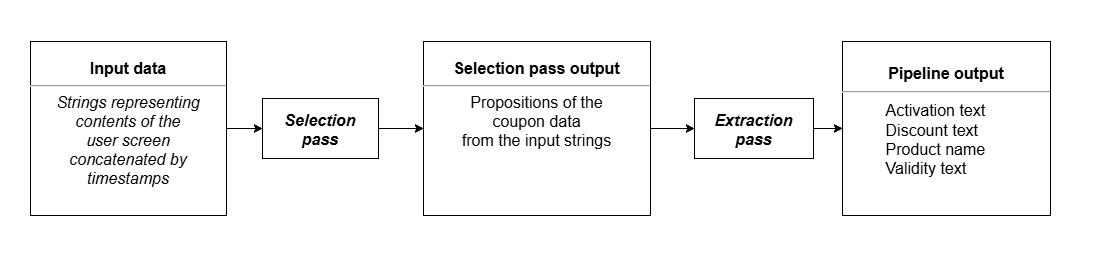
\includegraphics[width=1.0\linewidth]{bachelor_images/zpp.png}
    \caption{Pipeline graph}
    \label{fig:zpp}
\end{figure}

\begin{center}
   \begin{listing}
        \begin{minted}[frame=single,
                       framesep=3mm,
                       linenos=true,
                       xleftmargin=21pt,
                       tabsize=4]{js}
        {     
            "texts": ['Wasch-', '&', 'Reinigungsmittel', 'Vor',
            'Aktivierung', 'bitte', 'Hinweise', 'lesen.',
            'Deos,', 'Duschen,', 'Badezusätze', '&', 'Bodylotions',
            'Vor', 'Aktivierung', 'bitte', 'Hinweise', 'lesen.']
        }
        \end{minted}
        \caption{Pipeline input} 
        \label{list:sel-input}
    \end{listing}
\end{center}

\section{BERT family of models}
The widespread adoption of BERT~\cite{BERT_hf} has led to numerous architectural variants. Beyond the larger BERT-Large (around 300M parameters) and multilingual adaptations, efforts have focused on enhancing performance, e.g. RoBERTa~\cite{RoBERTa}, which outperforms vanilla BERT through extended pretraining and improving efficiency, e.g. ALBERT~\cite{ALBERT}, which reduces parameters to  around 12M~\cite{ALBERT_hf}.
Additionally, during our research, ModernBERT~\cite{ModernBERTPaper} was released, offering advancements such as extended context length of 8,192 tokens, faster inference, and superior performance on benchmark tasks. On top of that, it was still comparable with the base model, having around 150M parameters~\cite{ModernBERThf}.
After evaluating these variants, we selected the BERT-base multilingual model with 179M parameters~\cite{BERT_multiling}. This decision was driven mostly by the fact that all of the other mentioned models lacked multilingual support, making BERT-base really the only model that would only require fine-tunings on our data to work.

\section{Fine Tuning}
We implemented independent training for both BERT models in our pipeline. This approach provides several key advantages:

\begin{itemize}
    \item \textbf{Isolated Error Penalization}: Each model is only penalized for its own mistakes during training. Joint training could distort the selection model's loss function due to errors propagating from the extraction pass.
    
    \item \textbf{Data Integrity}: The extraction model trains on accurate intermediate representations, preventing potential bias from the selection model's imperfect predictions during joint training.
    
    \item \textbf{Practical Benefits}:
    \begin{itemize}
        \item Simplified implementation, compared to end-to-end training
        \item Greater control over each model's learning process
        \item Easier hyperparameter tuning for individual components
    \end{itemize}
\end{itemize}

This modular training strategy ensures both models reach their optimal performance without compromising each other's learning objectives.
\subsection{Fine-tuning methodology} \label{FTMethodologyBert}
Both selection and extraction models were trained on a dataset comprising data from four retail applications: DM, Lidl, Rewe, and Rossmann. The dataset was split 80\%--20\% for training and testing respectively, following common practice~\cite{pp}, with evaluation performed after each epoch. All fine-tuning experiments were conducted under the assumption that final model performance would be benchmarked on separate datasets from Edeka and Penny applications to maintain independence between training and evaluation data.
In total, we conducted four different experiments:

\begin{enumerate}
    \item \textbf{General Fine-tuning}:
    
    Main goal of this experiment was to establish baseline performance metrics. Additionally, this experiment was used as a basis to abandon
    Curriculum learning and JSON format approaches. It was conducted by fine-tuning models on combined data from all four applications.
    
    \item \textbf{Per-application Fine-tuning}:

    In this experiment, we wanted to examine cross-application generalization capabilities of our pipeline. To do this, we fine-tuned individual models separately on each application's data, and then tested them on other applications to measure similarities between datasets. This measurement was based on how well model trained on app X behaves on test dataset containing data from all four apps.
    
    \item \textbf{Incremental Separate Fine-tuning}:

    This was the first of two experiments used to see, how easily our solution could be generalized/extended. To conduct it, we performed four consecutive fine-tunings on each model:

    \begin{enumerate}
        \item Base model fine-tuned only on DM data
        \item Subsequent fine-tuning on Lidl data
        \item Additional fine-tuning on Rewe data
        \item Final fine-tuning on Rossmann data
    \end{enumerate}
    This way, we were able to see whether models gain more knowledge when presented with new sources of data or they loose it.
    
    \item \textbf{Incremental Combined Fine-tuning}:

    Idea behind our last experiment was similar to the Incremental Separate Fine-tuning, but this time we were adding new data to the training dataset, instead of changing them. This was intended as a way to prevent models from forgetting previously learned patterns. For that, we performed the following fine-tunings:
    \begin{enumerate}
        \item Initial fine-tuning on DM data only
        \item Subsequent fine-tuning on combined DM + Lidl data
        \item Additional fine-tuning on DM + Lidl + Rewe data
        \item Final fine-tuning on all four applications' data
    \end{enumerate}
\end{enumerate}

\subsection{Selection pass specifics}
Beyond the basic fine-tuning approach, we conducted two additional experiments with the selection pass model:

\begin{enumerate}
    \item \textbf{XML Tree Preservation} \cite{JSON_code}:
    
    When working with data grouped by timestamps, we loose the information about the relations between different elements on the user's screen. With XML tree preservation, we wanted to see if maintaining this information would improve coupon detection. To perform this experiment, we created special datasets, where screen content strings were wrapped in JSON structures simulating the XML hierarchy.

    Ultimately, we decided to abandon this approach for two reasons: first of all, it was performing worse than the original approach, called \emph{plain-text} (see plots \ref{fig:s_elg}, \ref{fig:e_epg}, \ref{fig:s_erg}). Second of all, wrapping everything in JSON structure introduced more text, which lead to bigger dataset sizes. As a result, fine-tunigs were longer and more costly, with no clear benefit.
    
    \item \textbf{Token Distribution Balancing} \cite{Curriculer}:
    
    First batches of data that we received from Murmuras had skewed data distribution. For many timestamps, only 10 \% of words contained in them were part of any coupon. As a result, models were not learning much, because labeling everything as UNKNOWN (not belonging to any coupon) was enough for more than 90 \% precision and recall. To counter this issue, we implemented a Curriculum Learning algorithm. The idea behind it was to first train models on datasets with manually balanced data distribution, and then, with more epochs, to increase the number of tokens that were not part of any coupon. Last epochs would be performed on the original dataset.

    At the end, this approach was also abandoned. Similarly, to the xml preservation, it was performing worse than the basic approach (see plots \ref{fig:s_elg}, \ref{fig:e_epg}, \ref{fig:s_erg}; models with "no-curr" are the ones fine-tuned without the curriculum learning). Additionally, later data batches from Murmuras were free from that flaw. Most of the timestamps had around 30 \% {-} 50 \% or more of words that were a part of some coupon.
\end{enumerate}

\section{Selection pass fine-tuning results}
General fine-tuning experiment demonstrated that a simple data representation without any class balancing yielded the best results, with the model without XML tree preservation and Curriculum learning reached 97 \% precision and almost 99 \% recall (see plots \ref{fig:s_elg}, \ref{fig:s_epg} and \ref{fig:s_erg}) As a consequence, we decided to abandon both the JSON format and the Curriculum Learning approach. Furthermore, subsequent experiments were conducted using 10 epochs instead of 30, as higher epoch counts led to increasing loss values for the base model.

For per-application fine-tuning, models generally performed poorly. Almost all models didn't suprass 20 \% in recall metric. An exception was the model trained on the Lidl dataset, with over 60\% recall (see plot \ref{fig:s_ers}).

In both incremental fine-tuning scenarios, although the model initially trained on DM data struggled with classification (almost 0 \% recall), further fine-tuning significantly improved its recall, with best result for separate fine-tunings being 72 \%  for Rossmann fine-tuning, and 87 \% in case of combined fine-tuning for also the Rossman fine-tuning. This suggests that it is possible to extend the model's functionality with minimal effort through simple fine-tuning (see plots \ref{fig:s_eras} and \ref{fig:s_erag}).

\section{Extraction pass fine-tuning results}
In the general fine-tuning setting, the extraction pass was learned smoothly. A potential concern, however, is the simultaneous increase in loss, recall, and precision, which may indicate slight overfitting (see plots \ref{fig:e_elg}, \ref{fig:e_epg}, \ref{fig:e_erg}).

The single-application experiment produced results similar to those observed in the selection pass. Once again, the model fine-tuned on Lidl dataset performed best, with 64 \% recall (see plot \ref{fig:e_ers}).

For both types of incremental experiments, the results closely mirrored those of the selection pass. For separate fine-tuning, Rossmann fine-tuning reached 95 \% recall, and for combined one, 99 \% recall. However, in this case, fine-tuning on the Lidl dataset led to even greater performance improvements, making additional fine-tuning less impactful. This indicates that with the right dataset, a relatively small amount of data may be sufficient to expand the model’s capabilities (see plots \ref{fig:e_eras}, \ref{fig:e_erag}).

\chapter{Fine-tuned Llama model} \label{chap:llama}
Apart from the aforementioned BERT-based proposal, we have prepared a fine-tuned version of Llama\cite{meta-llama} model to measure its performance in the studied task as a scrapping tool. The following sections focus on our setup for this proposal and the achieved results.

\section{The choice of the model}
Our primary model selection criterion was the model size - we wanted it to be deployable on as many smartphones as possible. That is why we have rejected models with more than 1 billion parameters, like \emph{Gemma 2 2B}\cite{gemma2} or \emph{Qwen2 1.5B}\cite{yang2024qwen2technicalreport}. We have also decided not to use models with acceptable size, but insufficient performance, like the 360M variant of \emph{SmolLM2}\cite{smollm2}. \emph{GPT-Neo}\cite{gpt-neo} was disqualified due to the lack of support from the Unsloth tool. Finally, we have chosen the 1B variant of the already mentioned \emph{llama3.2}.

\section{Task setup}
We assumed that the model is expected to take the content of the text fields displayed to the user on the screen and return a list of coupons in JSON format described in section~\ref{sec:coupon_model}. Additionally, we have explored the model's performance when the prompt was enhanced with the task description. However, no significant gain was achieved by us this way. We will refer to the llama fine-tuned with the task description as \emph{llama-w} and to the llama fine-tuned without it as \emph{llama-wth}. The full description of the prompt format is given in\ref{llamaDsDesc}.
\section{Fine-Tuning}
The fine-tuning was performed on the Modal platform with the help of the Unsloth tool. We used the cross-entropy loss\cite{mao2023crossentropylossfunctionstheoretical} and the AdamW optimizer adapted for 8-bit cached values\cite{hf-bnb}. Finally, we have applied weight decay and used a linear learning rate scheduler. The split between training and evaluation samples in the datasets was 80:20.

\section{Results of the fine-tuning}
In this part, we will analyze only cross-entropy loss evaluated during the training here as the models' performance on our benchmark is described in section~\ref{benchmarkResults}. The detailed plots for fine-tuning results are available in Appendix~\ref{AppH}.
\subsection{Baseline fine-tuning}
The baseline fine-tuning was performed on the datasets from four apps: REWE, ROSSMANN, LIDL and DM. During the training, the test loss was computed on the datasets from PENNY and EDEKA applications.

During the training of llama-wth, we observe the constant decrease of the training loss. It reaches the value below 0.2 after 9 epochs (see plot~\ref{fig:llama-wth-loss}). The evaluation loss drops to the value around 0.7 after initial epochs and then grows slowly to reach a value around 0.8 after 10 epochs. The test loss reached a value close to 1.3 after the first epoch and continued to grow over the rest of the epochs. This suggests that the model is overfitting to the training data.
The llama-w training plot (see~\ref{fig:llama-w-loss}) shows us that the test loss is at approximately 1.25 after the first epoch, the evaluation loss is close to 0.6 in its minimum and the train loss value after 10 epochs is around 0.1. This is a significant improvement compared to llama-wth, however, the overfitting still occurs.

\subsection{Application-wise fine-tuning}
We have also tested the model's ability to generalize when the fine-tuning was performed on the dataset consisting of only one application. In this case, we have measured the training and evaluation loss on the data from the selected application, while the test loss was computed on the EDEKA and PENNY applications, as in the baseline experiment. Each experiment came in a variant with the task description inserted into the prompt and without it.

When training on the prompt without the description, the test loss was significantly higher than in case of training on 4 applications simultaneously (see plot~\ref{fig:llama-wth-appwise}). After the first epoch it reached a value around 2.95 in case of the dataset from ROSSMANN, between 2.8 and 2.9 in case of DM and REWE, and a value slightly lower than 1.8 in case of LIDL. It continued to grow in the following epochs.
However, when the training set contained the task description, the test loss for ROSSMANN after the first epoch was on the level comparable to experiments from the previous subsection and it dropped further to a value around 1.15 after several epochs. After that, it started to grow. In case of LIDL, REWE and DM, the test loss reached its minimum after the first epoch with value 1.15 (see plot~\ref{fig:llama-w-appwise}).

\subsection{Experiments}
Additionally, we have performed experiments similar to the ones in Section~\ref{FTMethodologyBert}. We have performed the incremental combined fine-tuning where every $K$ epochs we introduced a new application to the dataset. Additionally, we have conducted an incremental separate fine-tuning where the dataset was replaced each $K$ epochs. We will refer to the newly introduced portion of the data as \emph{increment}. The results are described in the following subsubsections.
\subsubsection{Incremental combined fine-tuning}
We have tested different sizes of increments: 15, 50 and 100 (see plots~\ref{fig:llama-inc-tot-15-eval}~\ref{fig:llama-inc-tot-50-eval}~\ref{fig:llama-inc-tot-100-eval}). The evaluation loss was computed on the same applications as in the train set. When the task description is missing, we see that in each case the evaluation loss stabilizes around 0.9. However, it is worth noticing that when increment size is equal to 15, the evaluation loss drops to a value around 0.5 and then increases while in case of the greater values it starts at higher level and is decreasing as the training progresses. The test loss seems to fluctuate between 1.2 and 1.3 in the case of an increment size equal to 15 (see~\ref{fig:llama-inc-15-test}), behave in a more stable way around 1.2 for size 50 (see~\ref{fig:llama-inc-50-test}) and stabilize around 1.2 when increment size is 100 (see~\ref{fig:llama-inc-100-test}).

When training with the task description the test loss fluctuates around 1.15, even for an increment of size 15, which suggests that the amount of the data required to fine-tune existing model to the new application might be small (see plots~\ref{fig:llama-inc-tot-15-test-w}~\ref{fig:llama-inc-tot-50-test-w}~\ref{fig:llama-inc-tot-100-test-w}).

\subsubsection{Fine-tuning with dataset replacements}
In this experiment, the evaluation loss was computed on the data from all apps used in the previous increments.
When training without the task description, the evaluation loss plots look similar regardless of increment size (see plots~\ref{fig:llama-inc-15-eval}~\ref{fig:llama-inc-50-eval}~\ref{fig:llama-inc-100-eval}). The evaluation loss is at first around 0.5, then it jumps to around 0.85, finally, after the last dataset substitution, it ends around 0.9. These visualizations allow us to suggest the hypothesis that the model \emph{forgets} the overfitted dataset-specific knowledge as it no longer sees the samples from this dataset. The test loss jumps to the value above 1.4 after the first dataset swap and then drops to the value around 1.15 (see plots~\ref{fig:llama-inc-15-test}~\ref{fig:llama-inc-50-test}~\ref{fig:llama-inc-100-test}). This suggests that this methodology might be considered an interesting alternative for standard fine-tuning.

Addition of the task description further decreases the test loss, to values below 1.1 in later epochs for an increment size of 10 (see~\ref{fig:llama-inc-10-test-w}), and even reached 1.05 in the case of larger increment sizes (see~\ref{fig:llama-inc-50-test-w} and~\ref{fig:llama-inc-100-test-w}).

\chapter{Benchmark and Results} \label{chap:benchmark}

The objective of our custom benchmark is to enable a fair comparison of the pipelines with respect to the quality of their outputs. To achieve this, the benchmark compares the coupons extracted by each pipeline against the ground truth data provided by Murmuras and counts the number of correctly extracted coupons. This is accomplished by computing the similarities between the generated and expected coupons and applying a simple greedy matching algorithm.

By leveraging the benchmark and conducting a series of additional evaluations, we were able to systematically identify the pipeline that delivered the most satisfactory overall performance.

\section{Coupon Similarity}

The coupon similarity metric employed in this work is based on comparing text fields using a string distance measure (for further details, see Appendix~\ref{app:coupon_sim}). The resulting similarity score ranges from 0, indicating completely different texts, to 1, indicating identical texts. An alternative approach was considered, in which a large language model (LLM) would be used to assess the similarity between the expected and generated outputs~\cite{llm-as-a-judge}. The motivation for this consideration is that the generative pipeline, based on a model such as Llama, could produce a semantically correct answer but in an incorrect format, resulting in a low string similarity score despite the answer being essentially correct. However, we were unable to identify any documented instance where the LLM-as-a-Judge technique was successfully applied to a task sufficiently similar to ours, and providing a thorough validation of this approach falls outside the scope of this thesis.

\section{Benchmarking Algorithm}

For each entry in the benchmarking dataset, the similarities between all expected and generated coupons are computed. The matching process then proceeds iteratively: at each step, the coupon pair with the highest similarity score is selected and marked as matched. The matched coupons are removed from their respective sets, and the next highest-scoring pair is selected from the remaining coupons. This process is repeated until the highest remaining similarity score falls below a predefined threshold. In this work, the threshold was set to 0.8. The benchmark returns the total number of expected, generated, and matched coupons across the entire benchmarking dataset.

\section{Logging}

The benchmark logs both the results for individual entries and any unexpected events encountered during processing. For instance, during the parsing of the pipeline’s JSON output, any cases of incorrectly formatted data or coupons containing unexpected fields are recorded in the logs.

\section{Benchmarking Results} \label{benchmarkResults}

By interpreting the number of expected coupons as the sum of true positives and false negatives, the number of generated coupons as the sum of true positives and false positives, and the number of matched coupons as the number of true positives, we can compute both recall and precision. Following discussions with Murmuras, it was determined that recall is the more important metric in our context, as correctly extracting as many coupons as possible is the primary objective, while false positives are considered to be of lesser concern.

In the figures presented in Appendix~\ref{app:pipeline_comp}, as well as in Figures~\ref{fig:quantization_effect_on_recall} and~\ref{fig:quantization_effect_on_precision}, the models are evaluated across six datasets. The Penny and Edeka datasets were used in their entirety, while for DM, Lidl, Rewe, and Rossmann, only the test splits were used.

For a detailed description of the datasets, see Chapter~\ref{chap:datasets}. Information on the BERT-based pipelines is provided in Chapter~\ref{chap:bert}, while the Llama-based pipelines are discussed in Chapter~\ref{chap:llama}.

\section{Pipeline Comparison}

Based on Figures~\ref{fig:berts_recall} and~\ref{fig:berts_precision}, BERT-top\_score emerged as the best-performing variant within the BERT-based pipelines. It consistently outperformed BERT-first in both recall and precision. While the comparison with BERT-concat is less clear-cut, BERT-top\_score achieved more than twice the recall on the DM dataset, which was a decisive factor in its overall evaluation. 

Similarly, Figures~\ref{fig:llama_wth_vs_w_recall} and~\ref{fig:llama_wth_vs_w_precision} show that Llama-wth outperforms Llama-w. While Llama-w demonstrated slightly better precision, recall was prioritized as the more important metric, as previously discussed. 

When comparing BERT-top\_score to Llama-wth (Figures \ref{fig:llama_vs_bert_recall} and \ref{fig:llama_vs_bert_precision}), the latter clearly emerges as the superior approach in terms of output quality.

Overall, the pipelines performed significantly better on the datasets they were trained on—namely DM, Lidl, Rewe, and Rossmann—compared to the previously unseen datasets, Penny and Edeka. However, Figures~\ref{fig:llama_vs_bert_recall} and~\ref{fig:llama_vs_bert_precision} suggest that the Llama-based pipelines exhibit a higher potential for generalization than their BERT-based counterparts.

\section{Llama Quantization Comparison}

After identifying Llama-wth as the best-performing pipeline variant, we evaluated several quantized versions of the underlying model—specifically \texttt{Q8\_0}, \texttt{Q4\_K\_M}, and \texttt{Q4\_0}~\cite{llama-cpp-quantization}—in terms of recall, precision, inference speed on a mobile device, and GGUF file size. 

The model speed was evaluated by running the Llama-wth model with various quantization schemes using the \texttt{llama.cpp} framework (see Chapter~\ref{chap:technologies}) with the default CPU backend on a Samsung A25 device equipped with 6~GB of RAM. An initial warm-up run was performed using a short prompt of approximately 10 tokens, during which 16 tokens were generated. For the actual measurement, a prompt of around 300 tokens—sampled from one of the datasets—was used, and the model generated 64 tokens.

Based on the results shown in Figures~\ref{fig:quantization_effect_on_recall},~\ref{fig:quantization_effect_on_precision},~\ref{fig:quantization_effect_on_model_speed}, and~\ref{fig:quantization_effect_on_gguf_file_size}, we found that quantization introduced no substantial degradation in output quality while offering clear improvements in inference speed and reduced model size. The latter also contributes to lower memory (RAM) usage during execution.

\chapter{Conclusion} \label{chap:conclusion}
\section{TODO}

\let\cleardoublepage\clearpage

\begin{appendices}

\chapter{BERT selection pass fine-tuning results} \label{AppC}
\begin{figure}[ht]
    \centering
    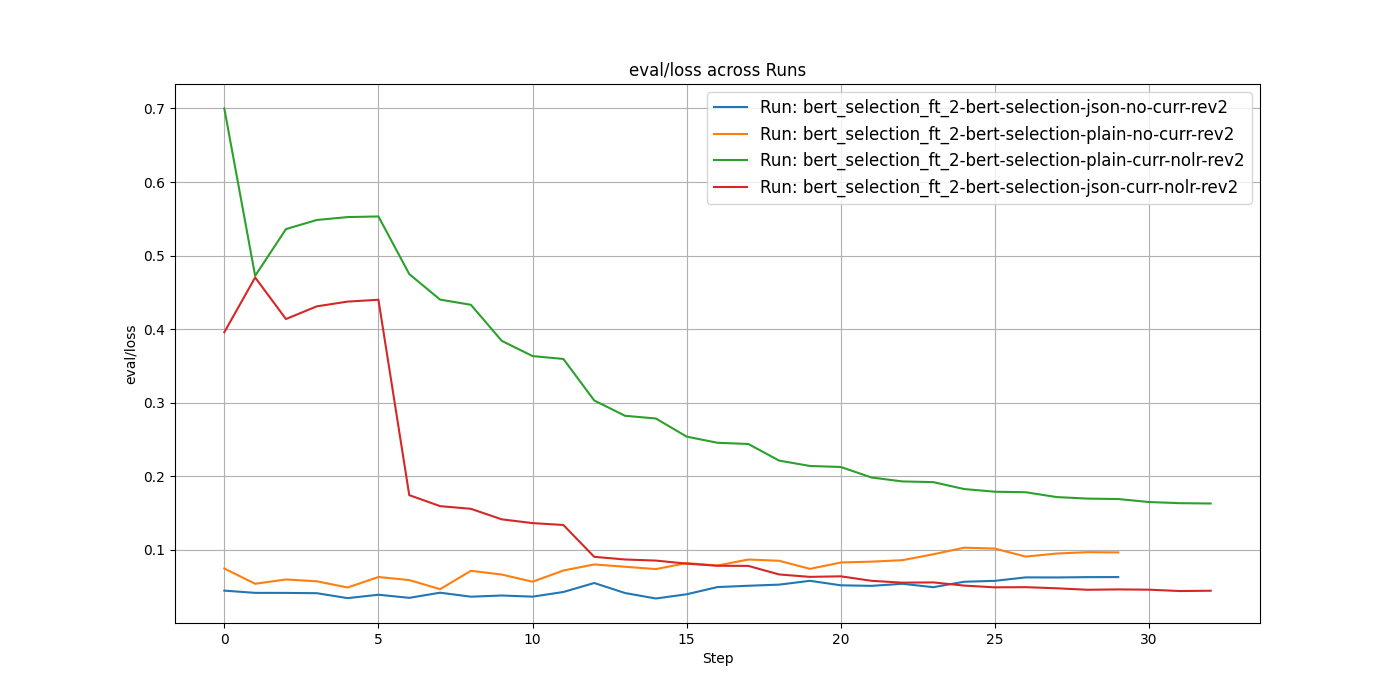
\includegraphics[width=0.8\linewidth]{bachelor_images/bert_ft/s_elg.png}
    \caption{Eval/loss statistics of selection pass during general training}
    \label{fig:s_elg}
\end{figure}
\begin{figure}[ht]
    \centering
    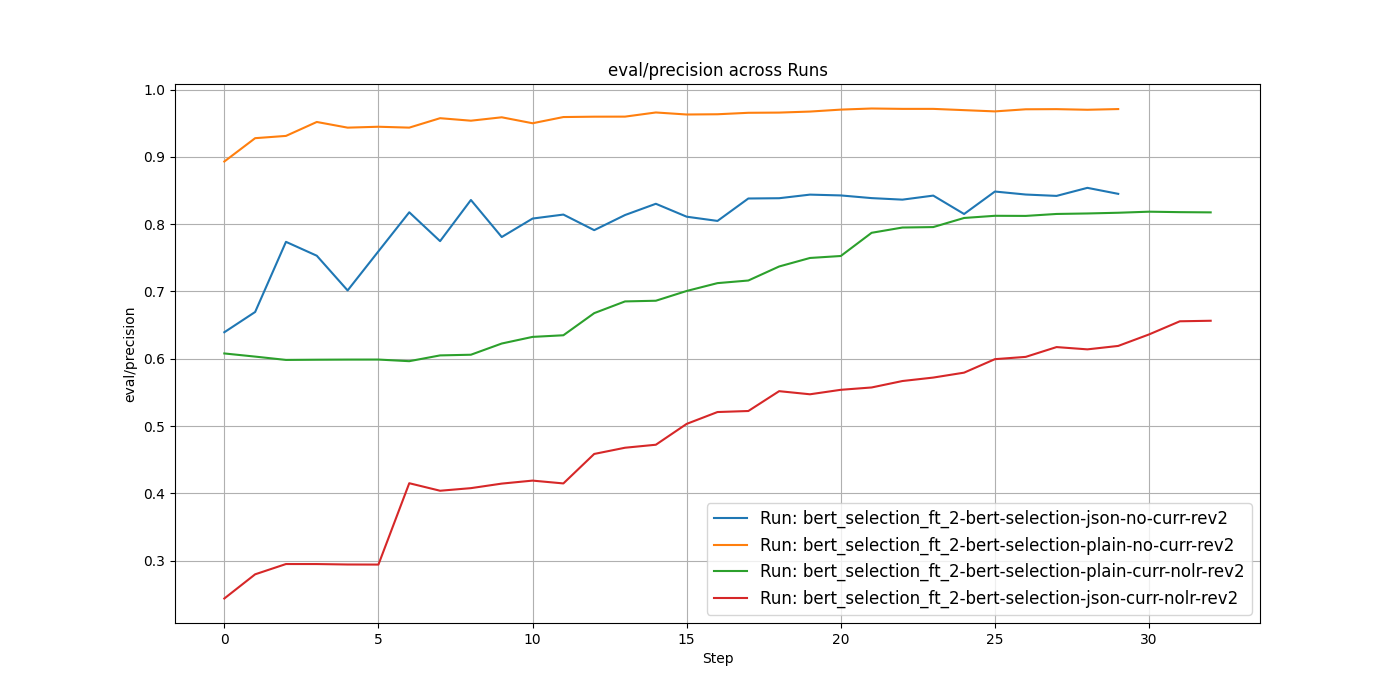
\includegraphics[width=0.8\linewidth]{bachelor_images/bert_ft/s_epg.png}
    \caption{Eval/precision statistics of selection pass during general training}
    \label{fig:s_epg}
\end{figure}
\begin{figure}[ht]
    \centering
    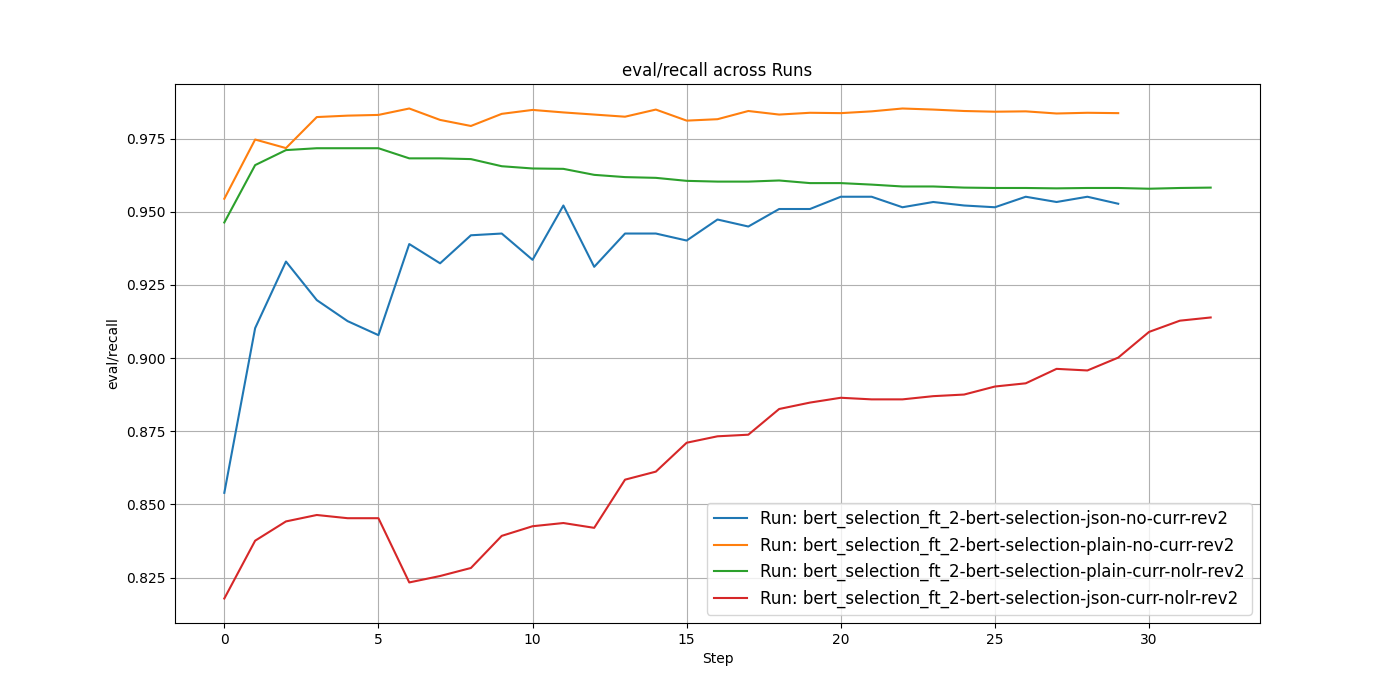
\includegraphics[width=0.8\linewidth]{bachelor_images/bert_ft/s_erg.png}
    \caption{Eval/recall statistics of selection pass during general training}
    \label{fig:s_erg}
\end{figure}

\begin{figure}[ht]
    \centering
    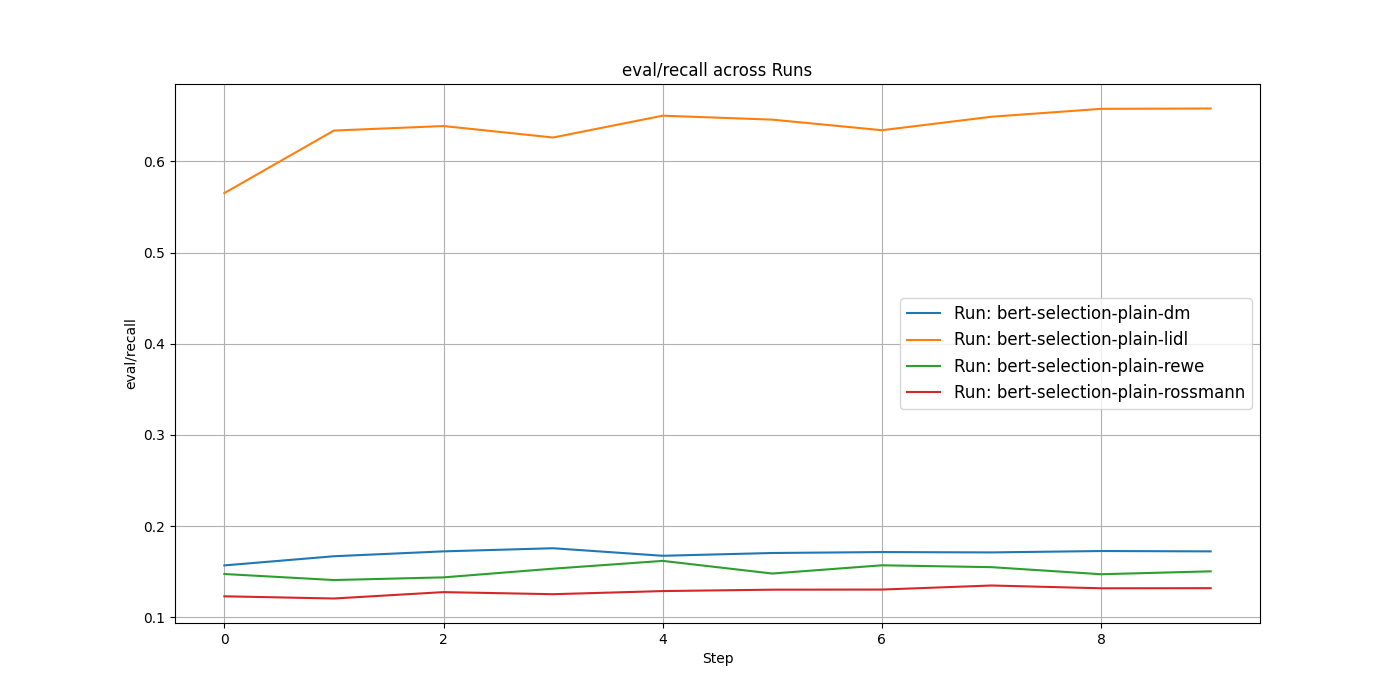
\includegraphics[width=0.8\linewidth]{bachelor_images/bert_ft/s_ers.png}
    \caption{Eval/recall statistics of selection pass during training on separate apps}
    \label{fig:s_ers}
\end{figure}

\begin{figure}[ht]
    \centering
    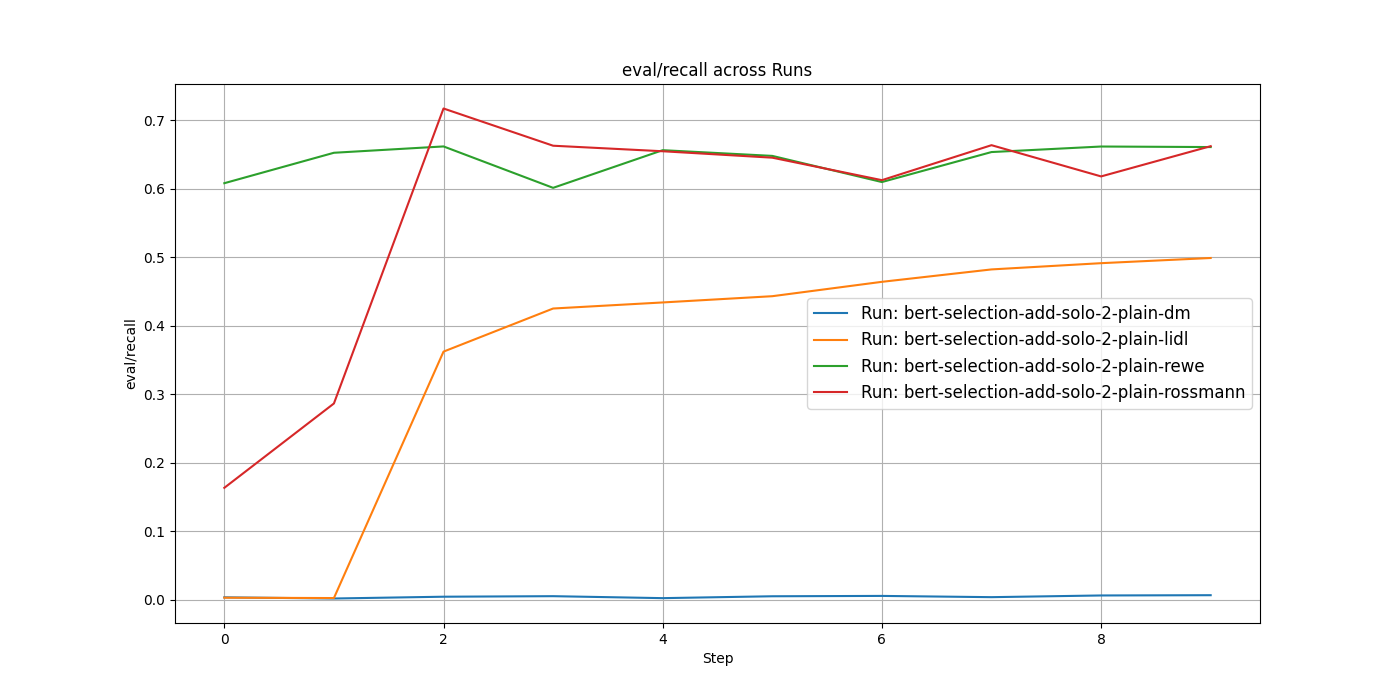
\includegraphics[width=0.8\linewidth]{bachelor_images/bert_ft/s_eras.png}
    \caption{Eval/recall statistics of selection pass during incremental separate training}
    \label{fig:s_eras}
\end{figure}

\begin{figure}[ht]
    \centering
    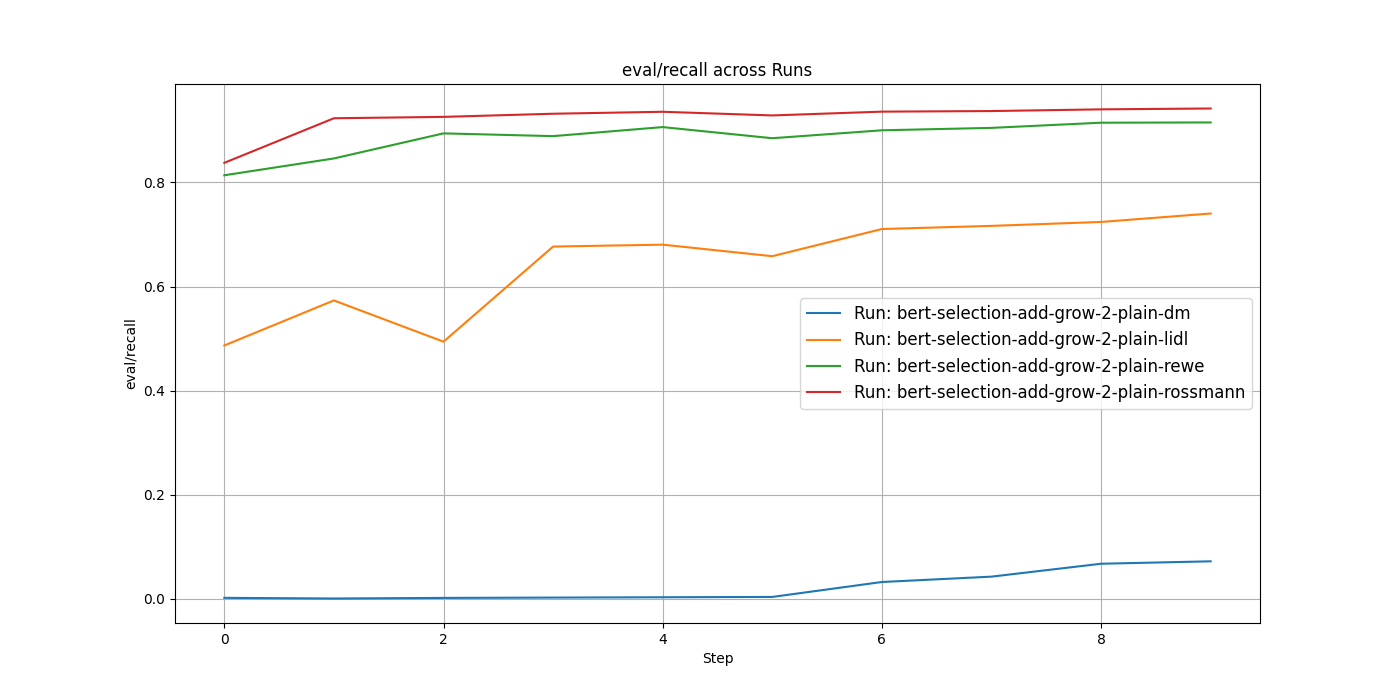
\includegraphics[width=0.8\linewidth]{bachelor_images/bert_ft/s_erag.png}
    \caption{Eval/recall statistics of selection pass during incremental combined training}
    \label{fig:s_erag}
\end{figure}

\chapter{BERT extraction pass fine-tuning results} \label{AppD}
\begin{figure}[ht]
    \centering
    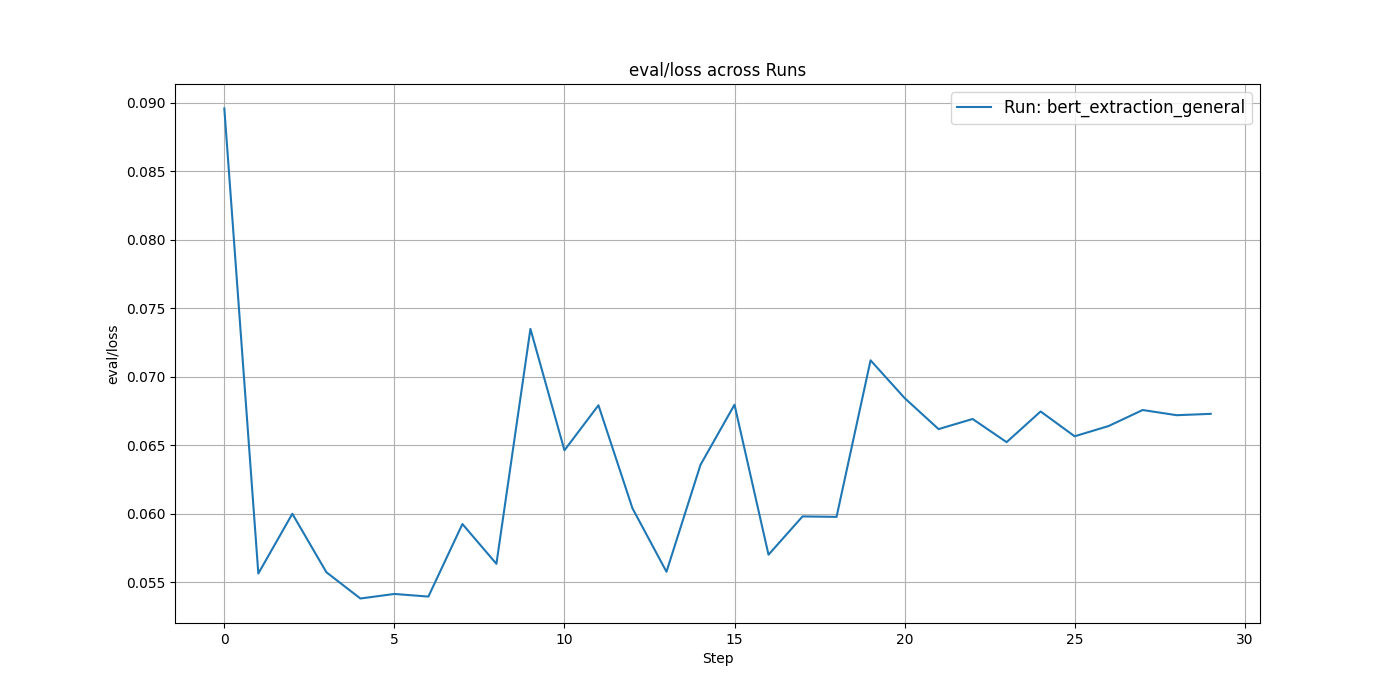
\includegraphics[width=0.8\linewidth]{bachelor_images/bert_ft/e_elg.png}
    \caption{Eval/loss statistics of extraction pass during general training}
    \label{fig:e_elg}
\end{figure}
\begin{figure}[ht]
    \centering
    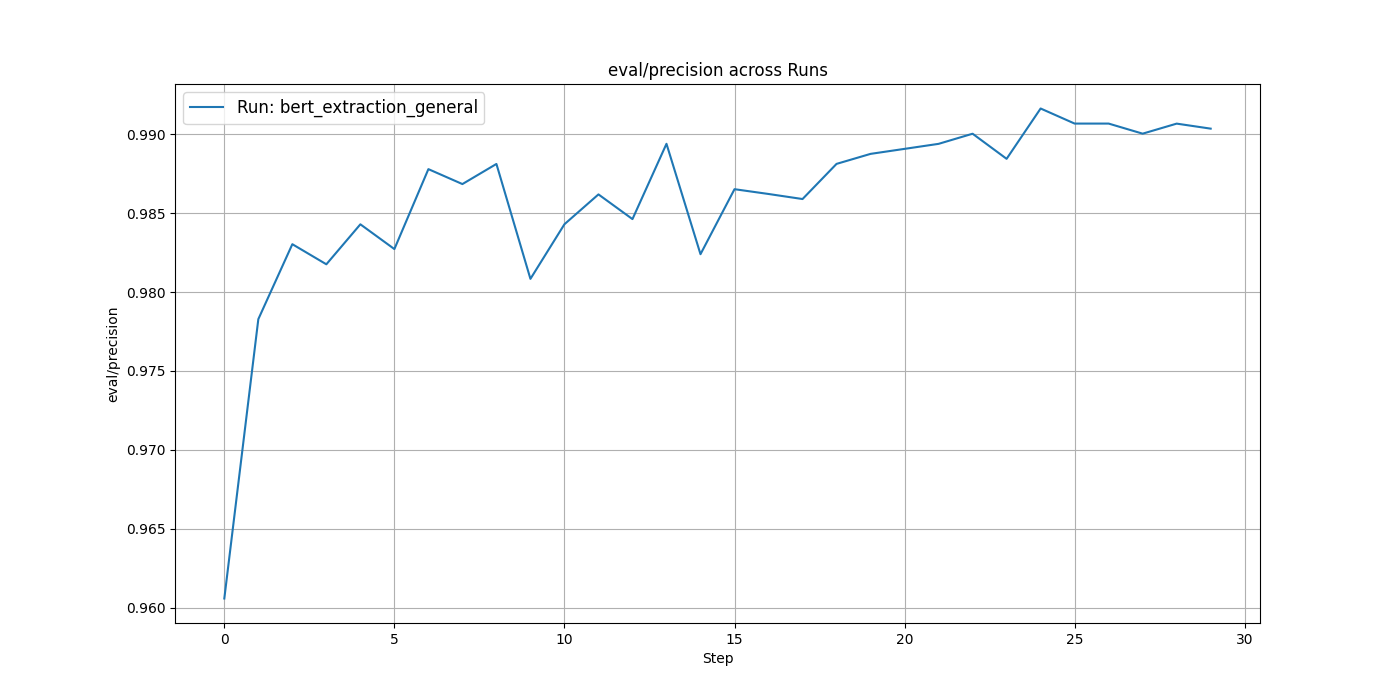
\includegraphics[width=0.8\linewidth]{bachelor_images/bert_ft/e_epg.png}
    \caption{Eval/precision statistics of extraction pass during general training}
    \label{fig:e_epg}
\end{figure}
\begin{figure}[ht]
    \centering
    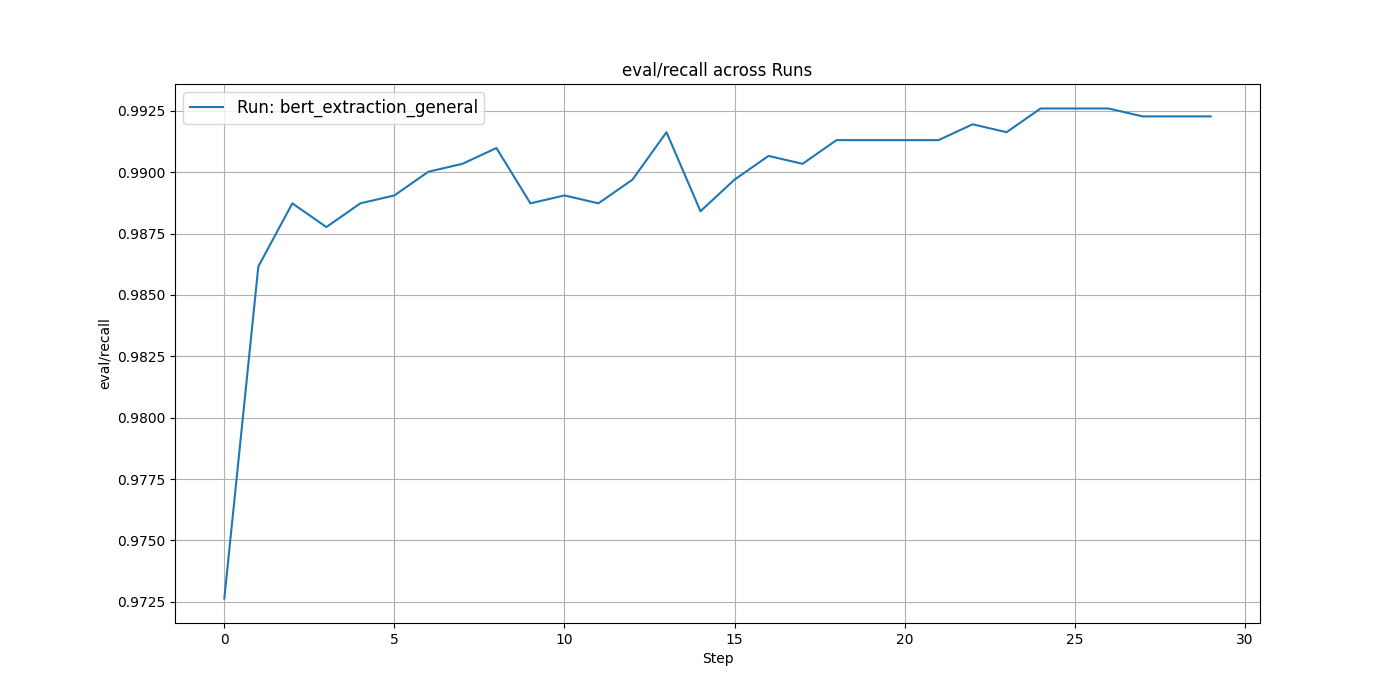
\includegraphics[width=0.8\linewidth]{bachelor_images/bert_ft/e_erg.png}
    \caption{Eval/recall statistics of extraction pass during general training}
    \label{fig:e_erg}
\end{figure}

\begin{figure}[ht]
    \centering
    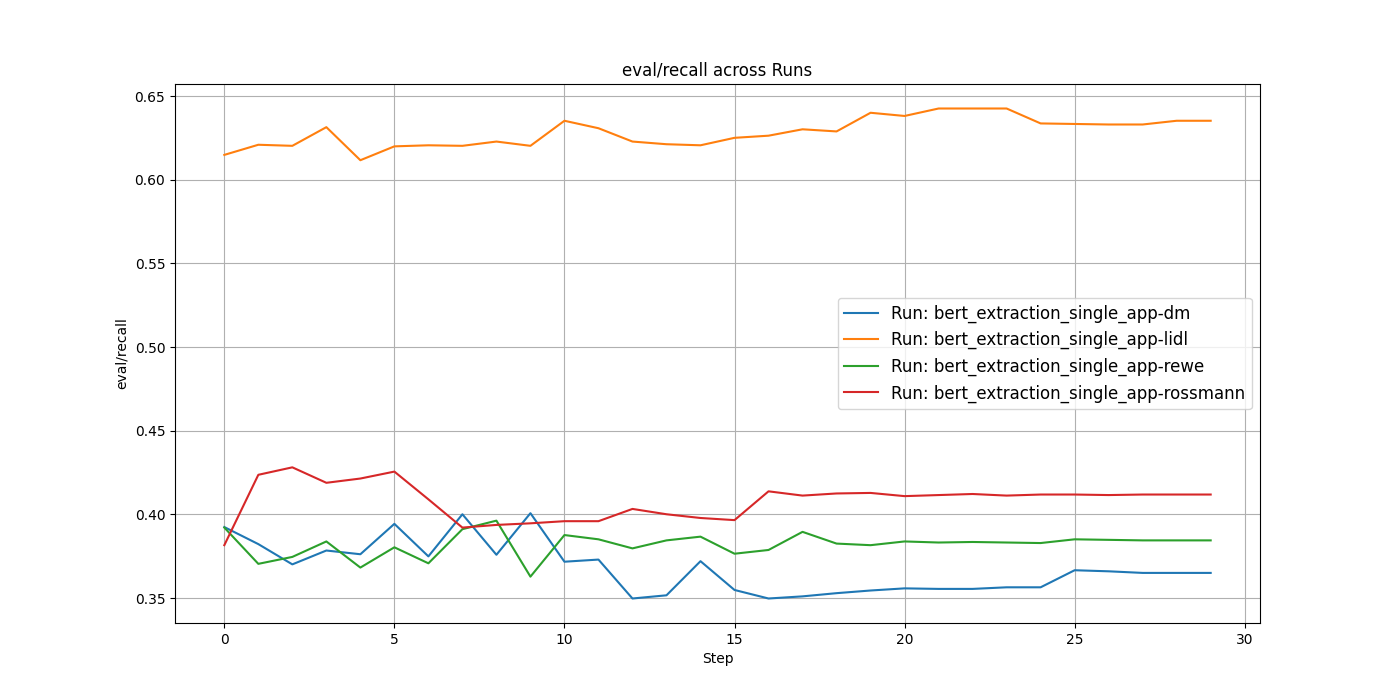
\includegraphics[width=0.8\linewidth]{bachelor_images/bert_ft/e_ers.png}
    \caption{Eval/recall statistics of extraction pass during separate training}
    \label{fig:e_ers}
\end{figure}

\begin{figure}[ht]
    \centering
    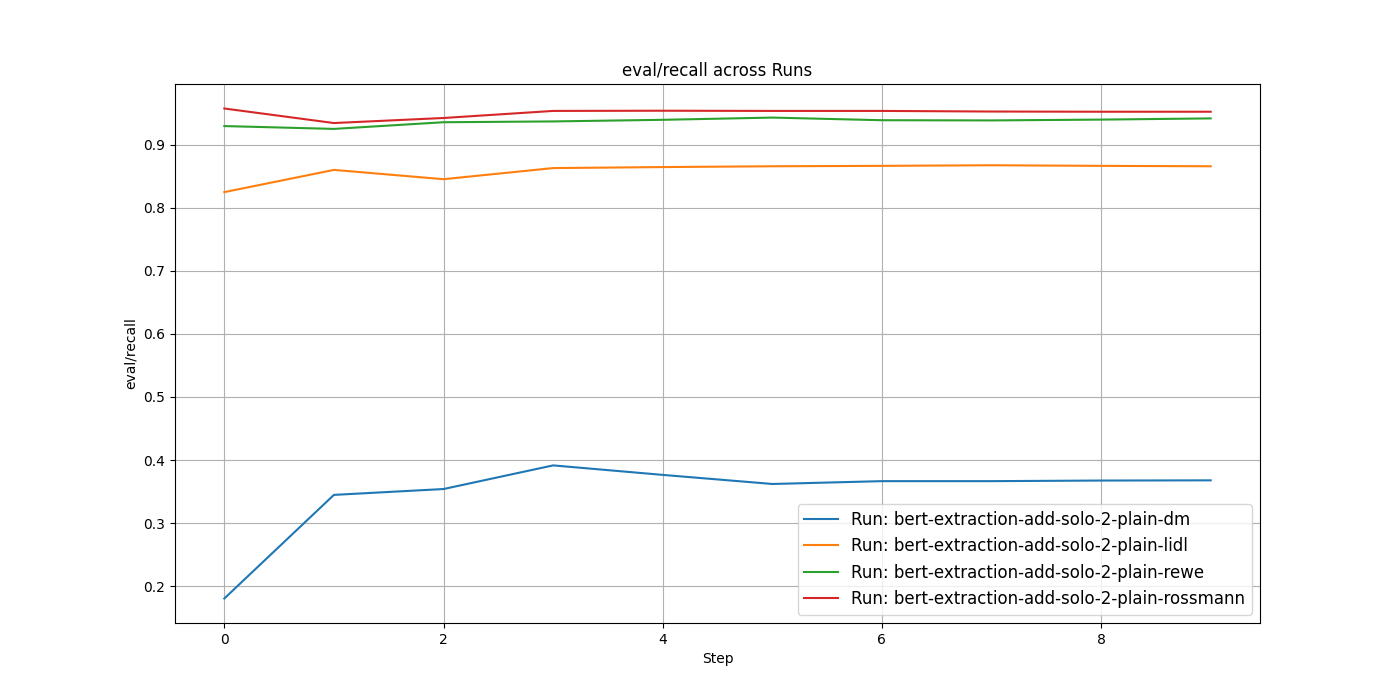
\includegraphics[width=0.8\linewidth]{bachelor_images/bert_ft/e_eras.png}
    \caption{Eval/recall statistics of extraction pass during incremental separate training}
    \label{fig:e_eras}
\end{figure}

\begin{figure}[ht]
    \centering
    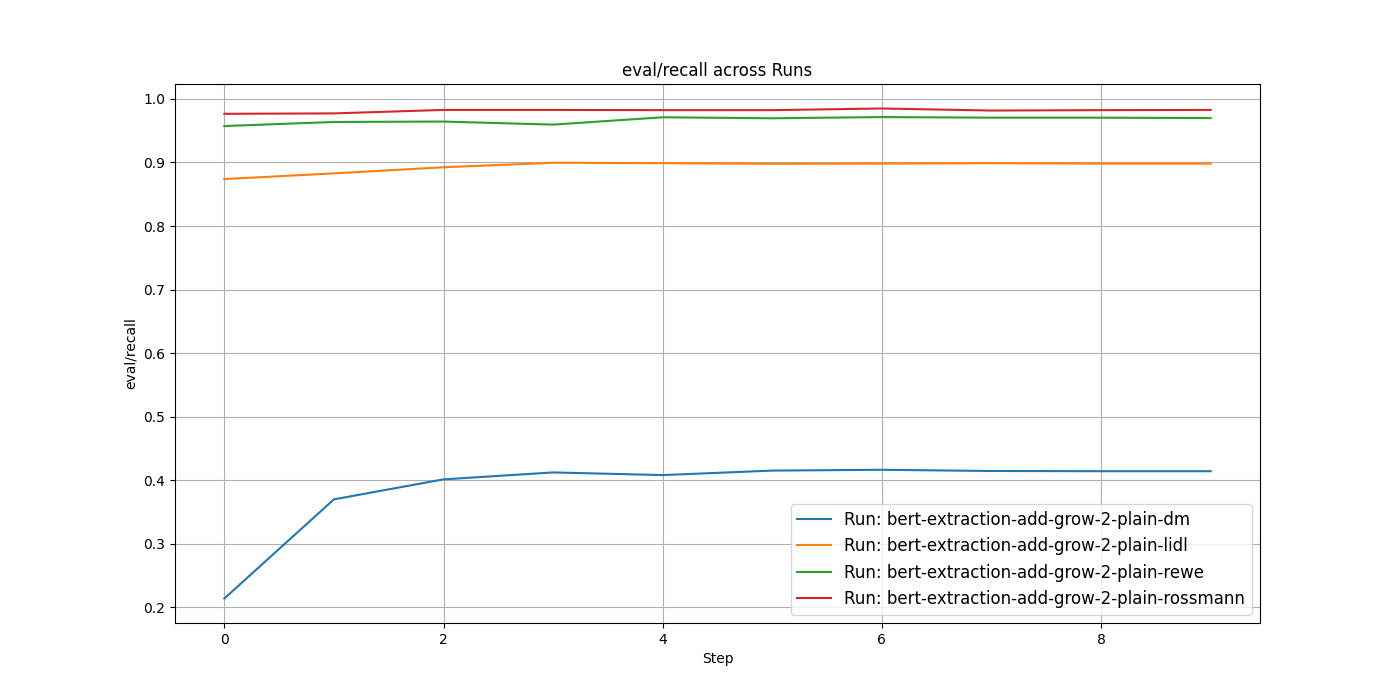
\includegraphics[width=0.8\linewidth]{bachelor_images/bert_ft/e_erag.png}
    \caption{Eval/recall statistics of extraction pass during incremental combined training}
    \label{fig:e_erag}
\end{figure}

\chapter{Coupon Similarity Metric} \label{app:coupon_sim}
The similarity between coupons is computed by comparing their textual fields using the \texttt{ratio()} method of Python's \texttt{difflib.SequenceMatcher} class~\cite{python-difflib}. The similarity computation algorithm is presented in two stages: first, the baseline approach is described, followed by an improved version. 

The input to the algorithm consists of an expected coupon and a generated coupon, both containing the text fields \texttt{PRODUCT-NAME}, \texttt{DISCOUNT-TEXT}, \texttt{VALIDITY-TEXT}, and \texttt{ACTIVATION-TEXT}.

\section{Baseline Approach}
The similarity of each text field is computed individually. For instance, if \texttt{text\_1} denotes the value of the \texttt{PRODUCT-NAME} field in the expected coupon and \texttt{text\_2} denotes the corresponding field in the generated coupon, their similarity is computed as follows:

\begin{lstlisting}[language=Python]
similarity = difflib.SequenceMatcher(a=text_1, b=text_2).ratio()
\end{lstlisting}

Each field is assigned a weight reflecting its relative importance: \texttt{PRODUCT-NAME} is weighted 0.4, \texttt{DISCOUNT-TEXT} is weighted 0.3, \texttt{VALIDITY-TEXT} is weighted 0.2, and \texttt{ACTIVATION-TEXT} is weighted 0.1. The final similarity score is calculated as the weighted sum of the individual field similarities.

However, this approach has a notable flaw. Consider the case where the expected coupon has only the \texttt{PRODUCT-NAME} field filled with the string \texttt{"a"}, while the generated coupon has the \texttt{PRODUCT-NAME} field filled with \texttt{"b"}; all other fields are empty. Despite the minimal information provided, the resulting similarity score would be 0.6, which overestimates the similarity.

\section{Improved Algorithm}
To mitigate this issue, the improved algorithm modifies how empty fields are handled. Specifically, if a given field is empty in both the expected and generated coupons, its contribution to the final similarity score is ignored. The final similarity score is then rescaled accordingly to reflect only the non-empty fields. For example, if both the \texttt{VALIDITY-TEXT} and \texttt{ACTIVATION-TEXT} fields are empty in both coupons, their similarities are considered to be 0, and the final similarity score is divided by 0.7, that is, the sum of the remaining fields' weights. In case the sum of remaining fields' weights is 0, the similarity of the coupons is set to 1.

\chapter{Pipeline Comparison Plots} \label{app:pipeline_comp}
\begin{figure}[ht]
    \centering
    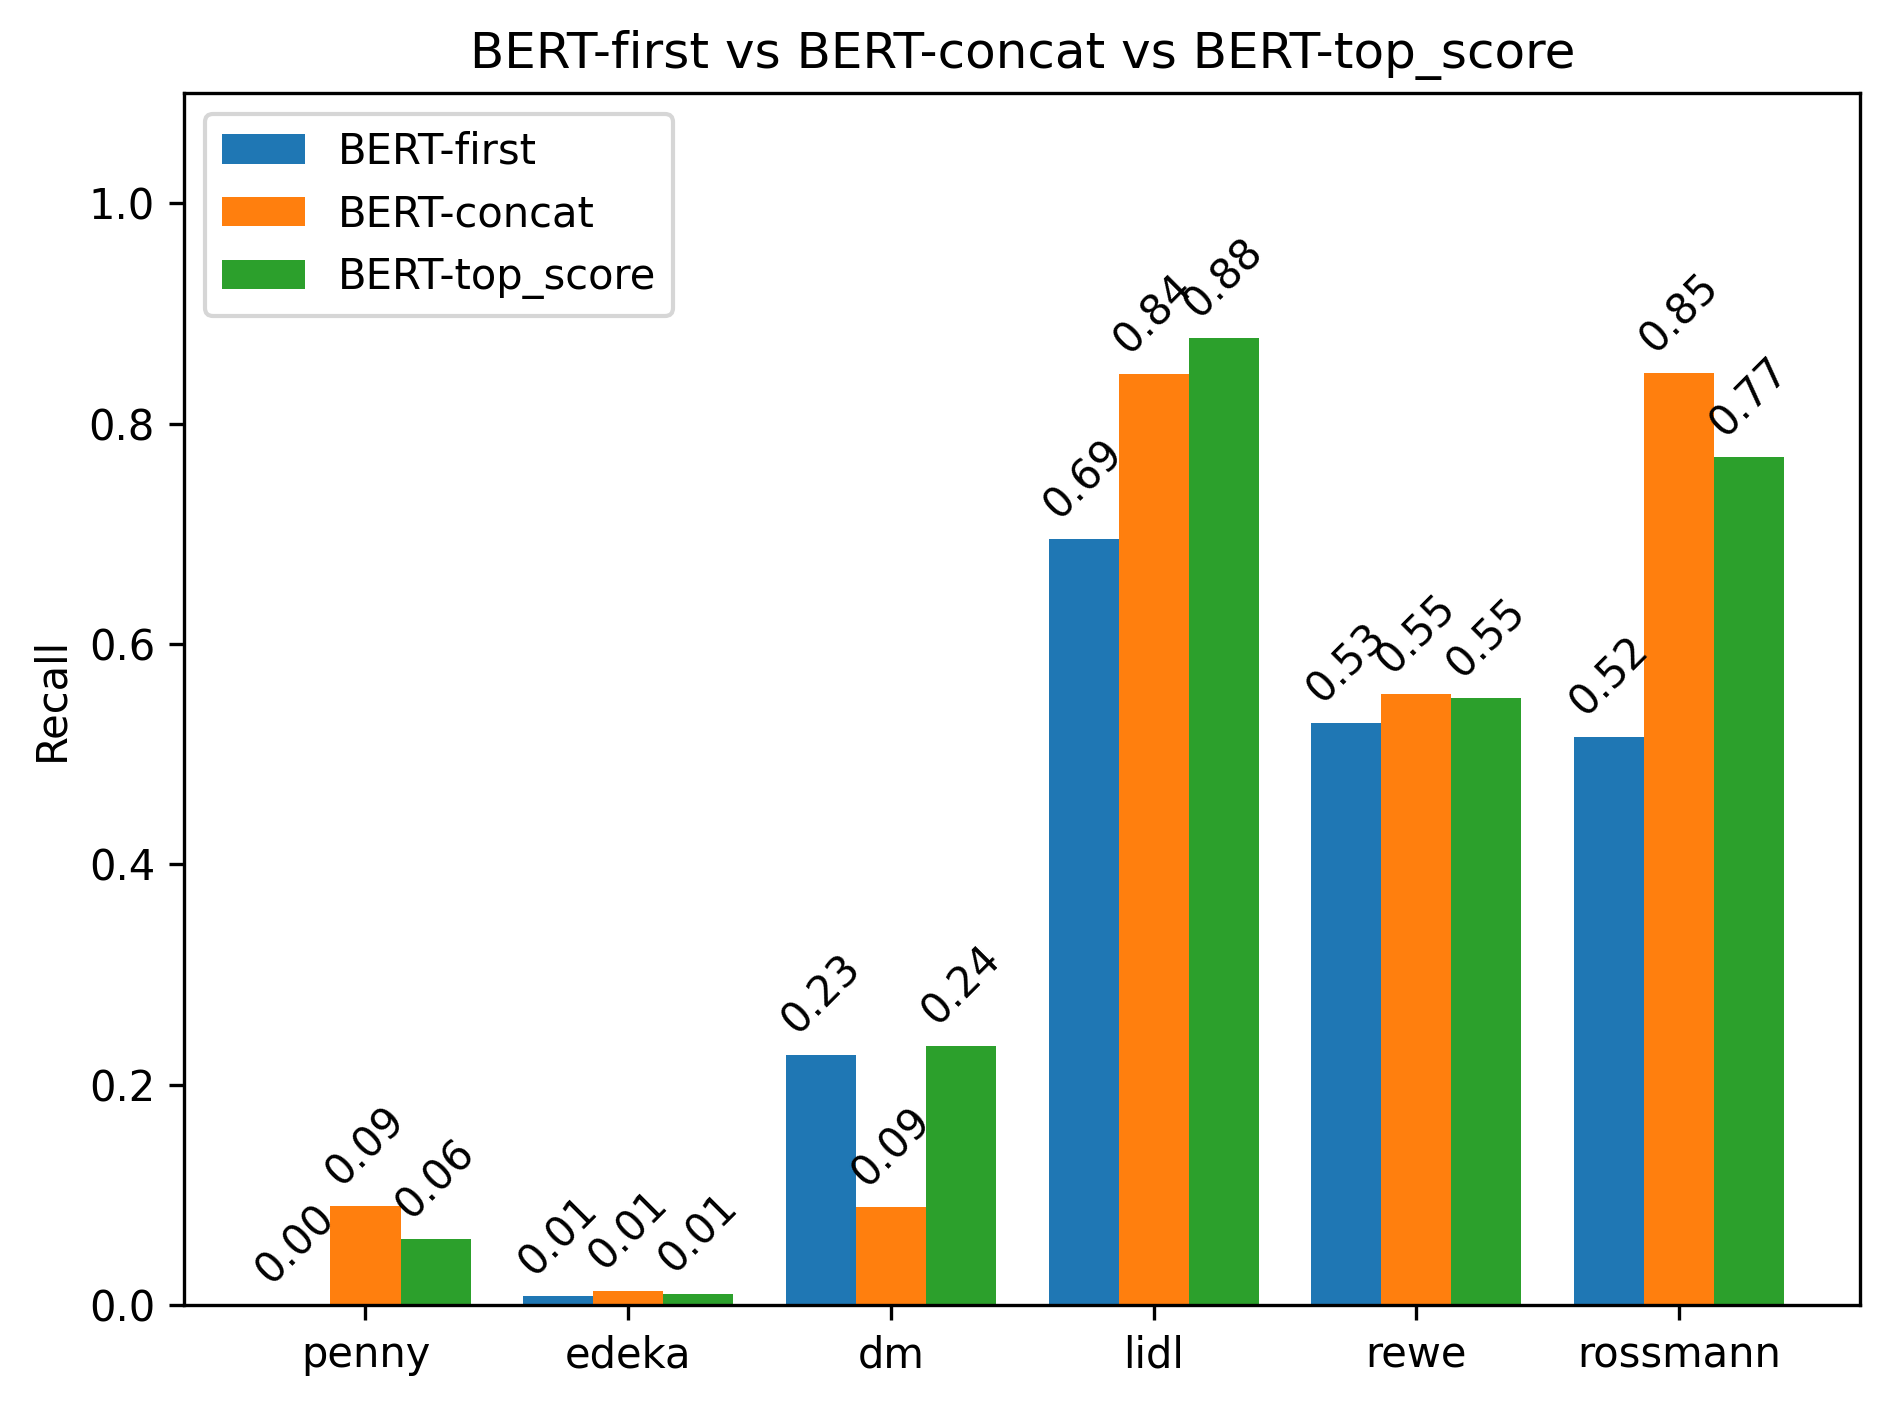
\includegraphics[width=0.8\linewidth]{bachelor_images/benchmark/berts_recall.png}
    \caption{BERT-first vs BERT-concat vs BERT-top\_score - recall}
    \label{fig:berts_recall}
\end{figure}

\begin{figure}[ht]
    \centering
    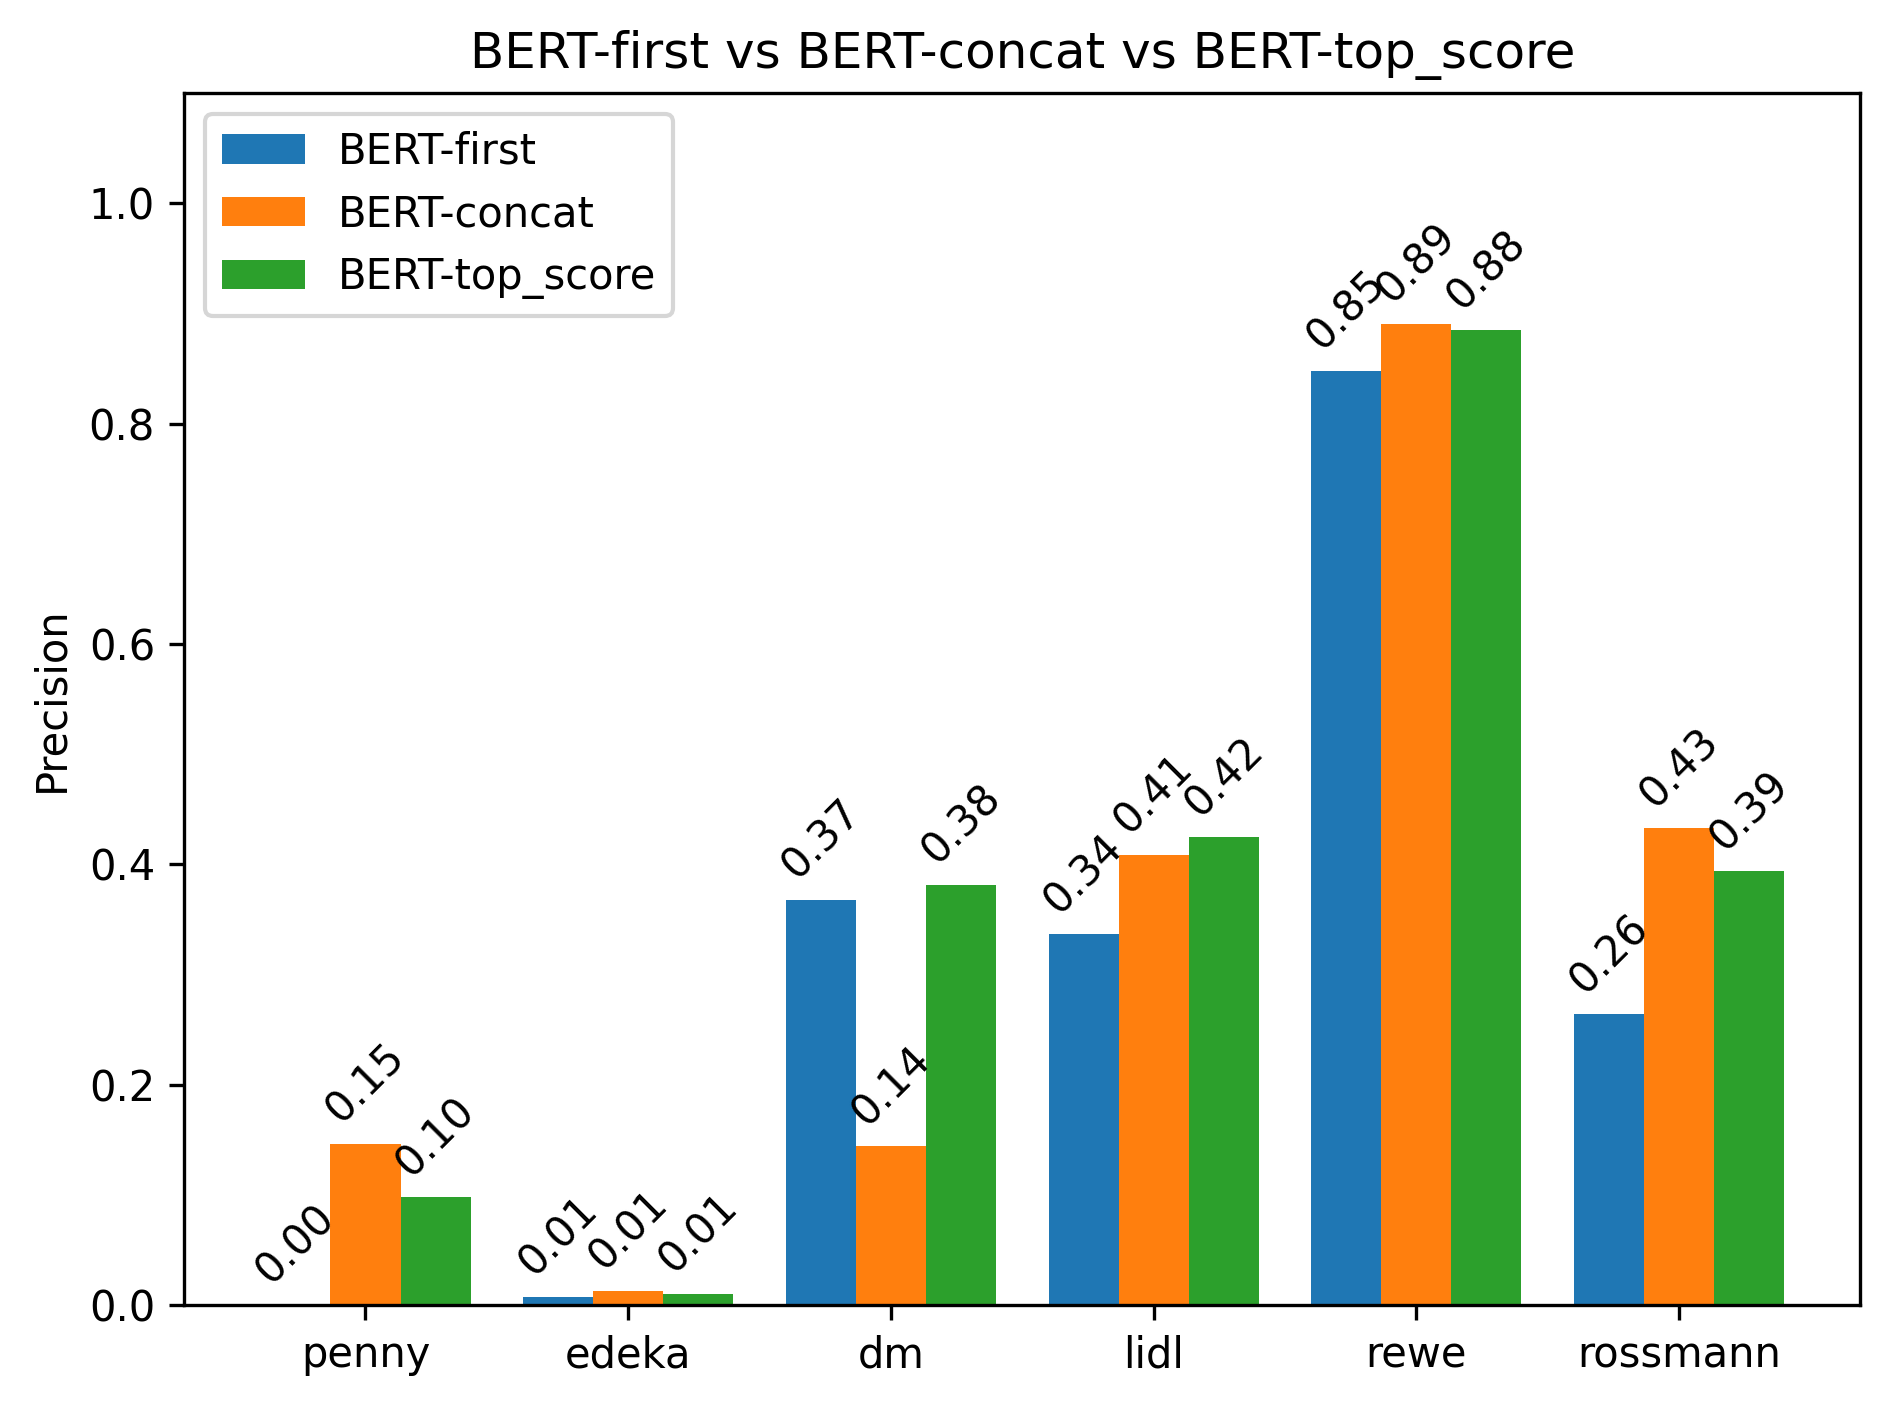
\includegraphics[width=0.8\linewidth]{bachelor_images/benchmark/berts_precision.png}
    \caption{BERT-first vs BERT-concat vs BERT-top\_score - precision}
    \label{fig:berts_precision}
\end{figure}

\begin{figure}[ht]
    \centering
    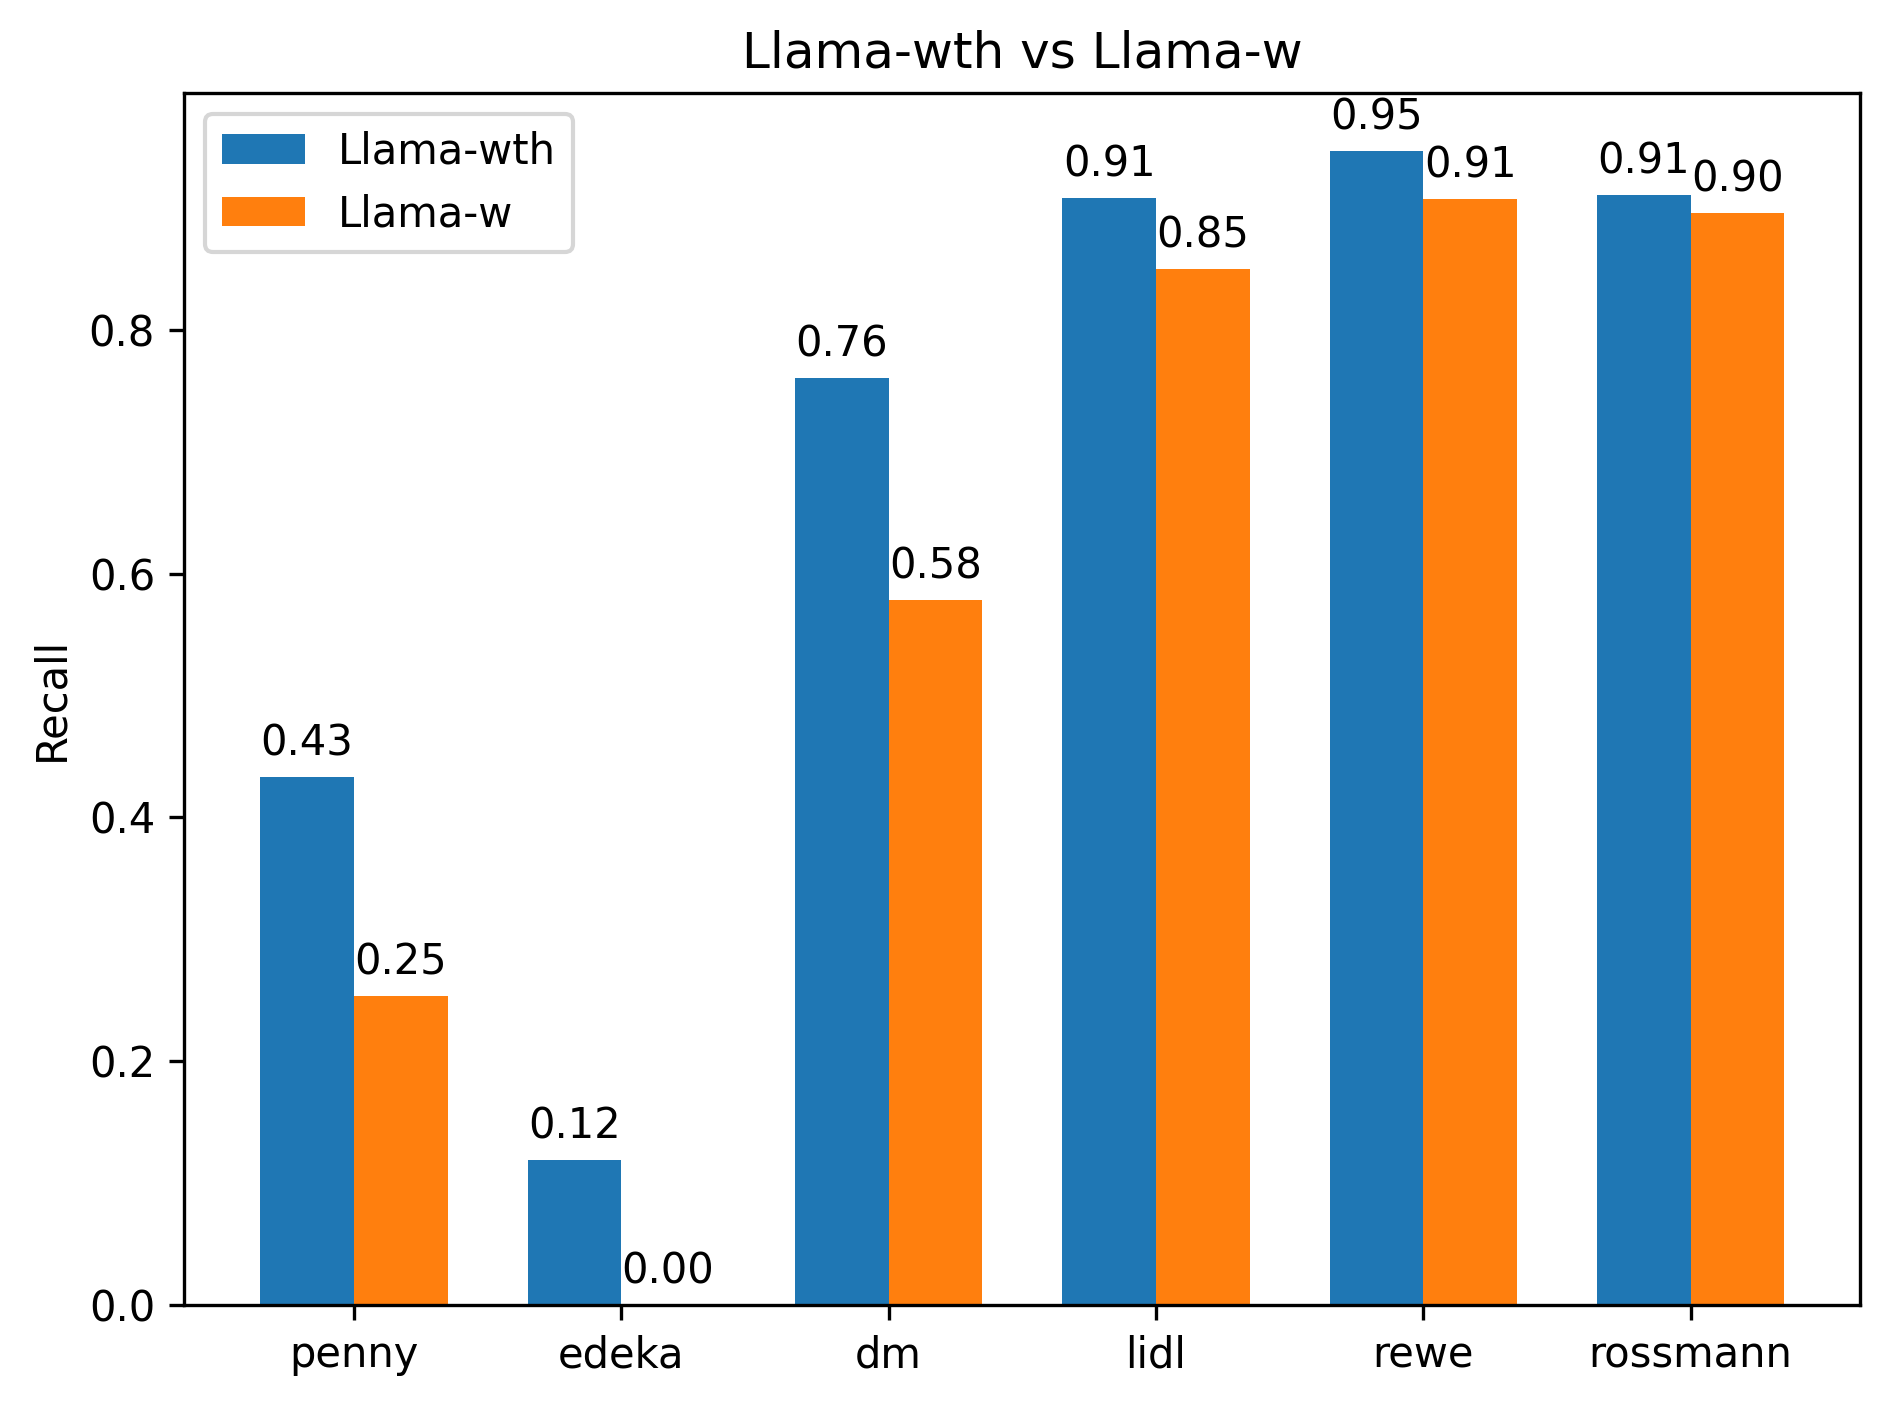
\includegraphics[width=0.8\linewidth]{bachelor_images/benchmark/llama_wth_vs_w_recall.png}
    \caption{Llama-wth vs Llama-w - recall}
    \label{fig:llama_wth_vs_w_recall}
\end{figure}

\begin{figure}[ht]
    \centering
    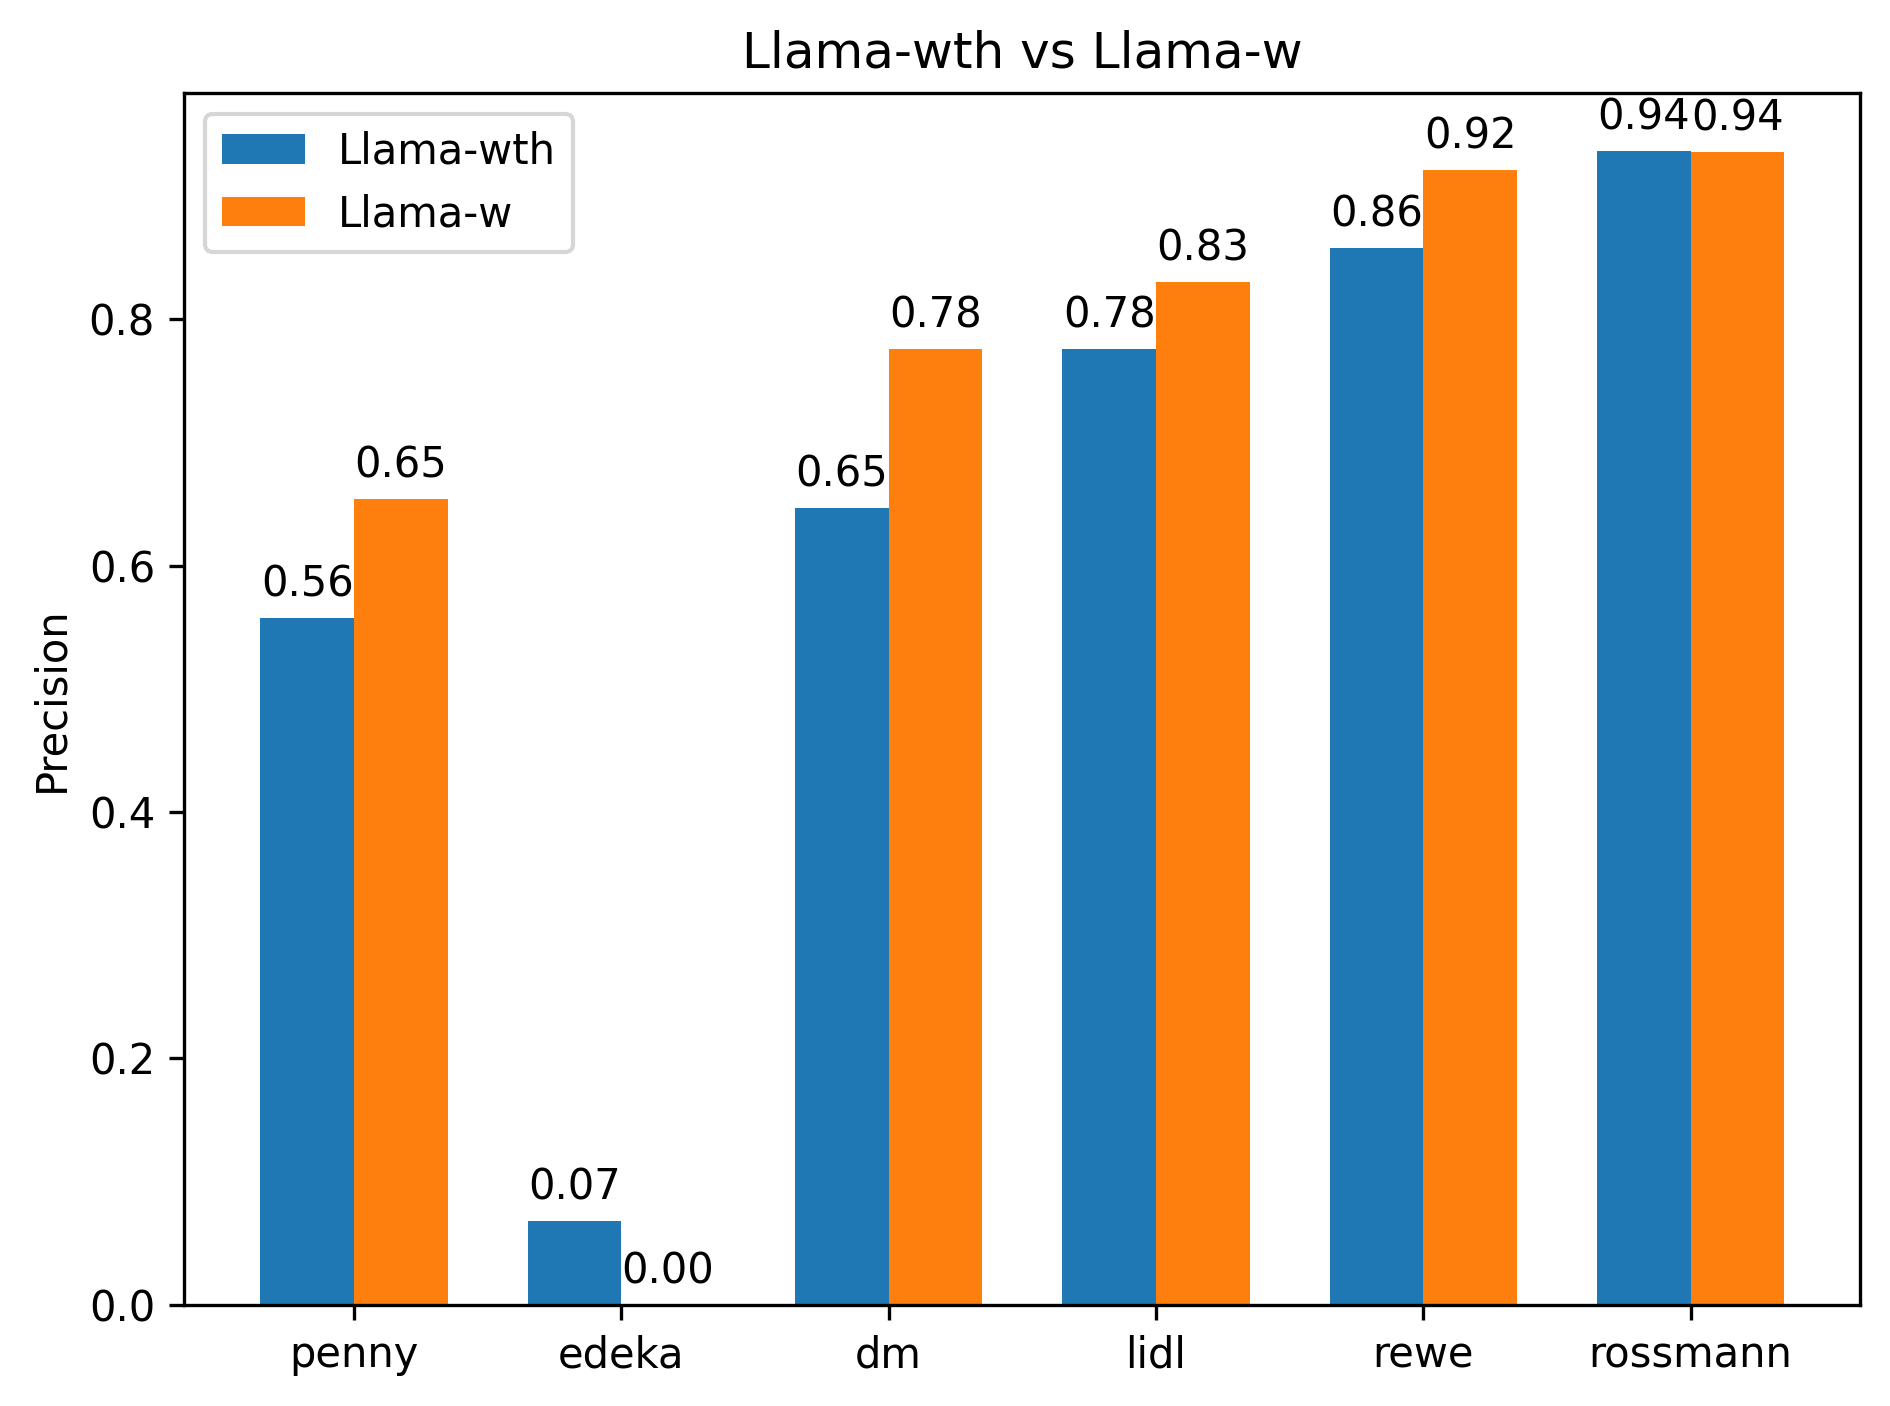
\includegraphics[width=0.8\linewidth]{bachelor_images/benchmark/llama_wth_vs_w_precision.png}
    \caption{Llama-wth vs Llama-w - precision}
    \label{fig:llama_wth_vs_w_precision}
\end{figure}

\begin{figure}[ht]
    \centering
    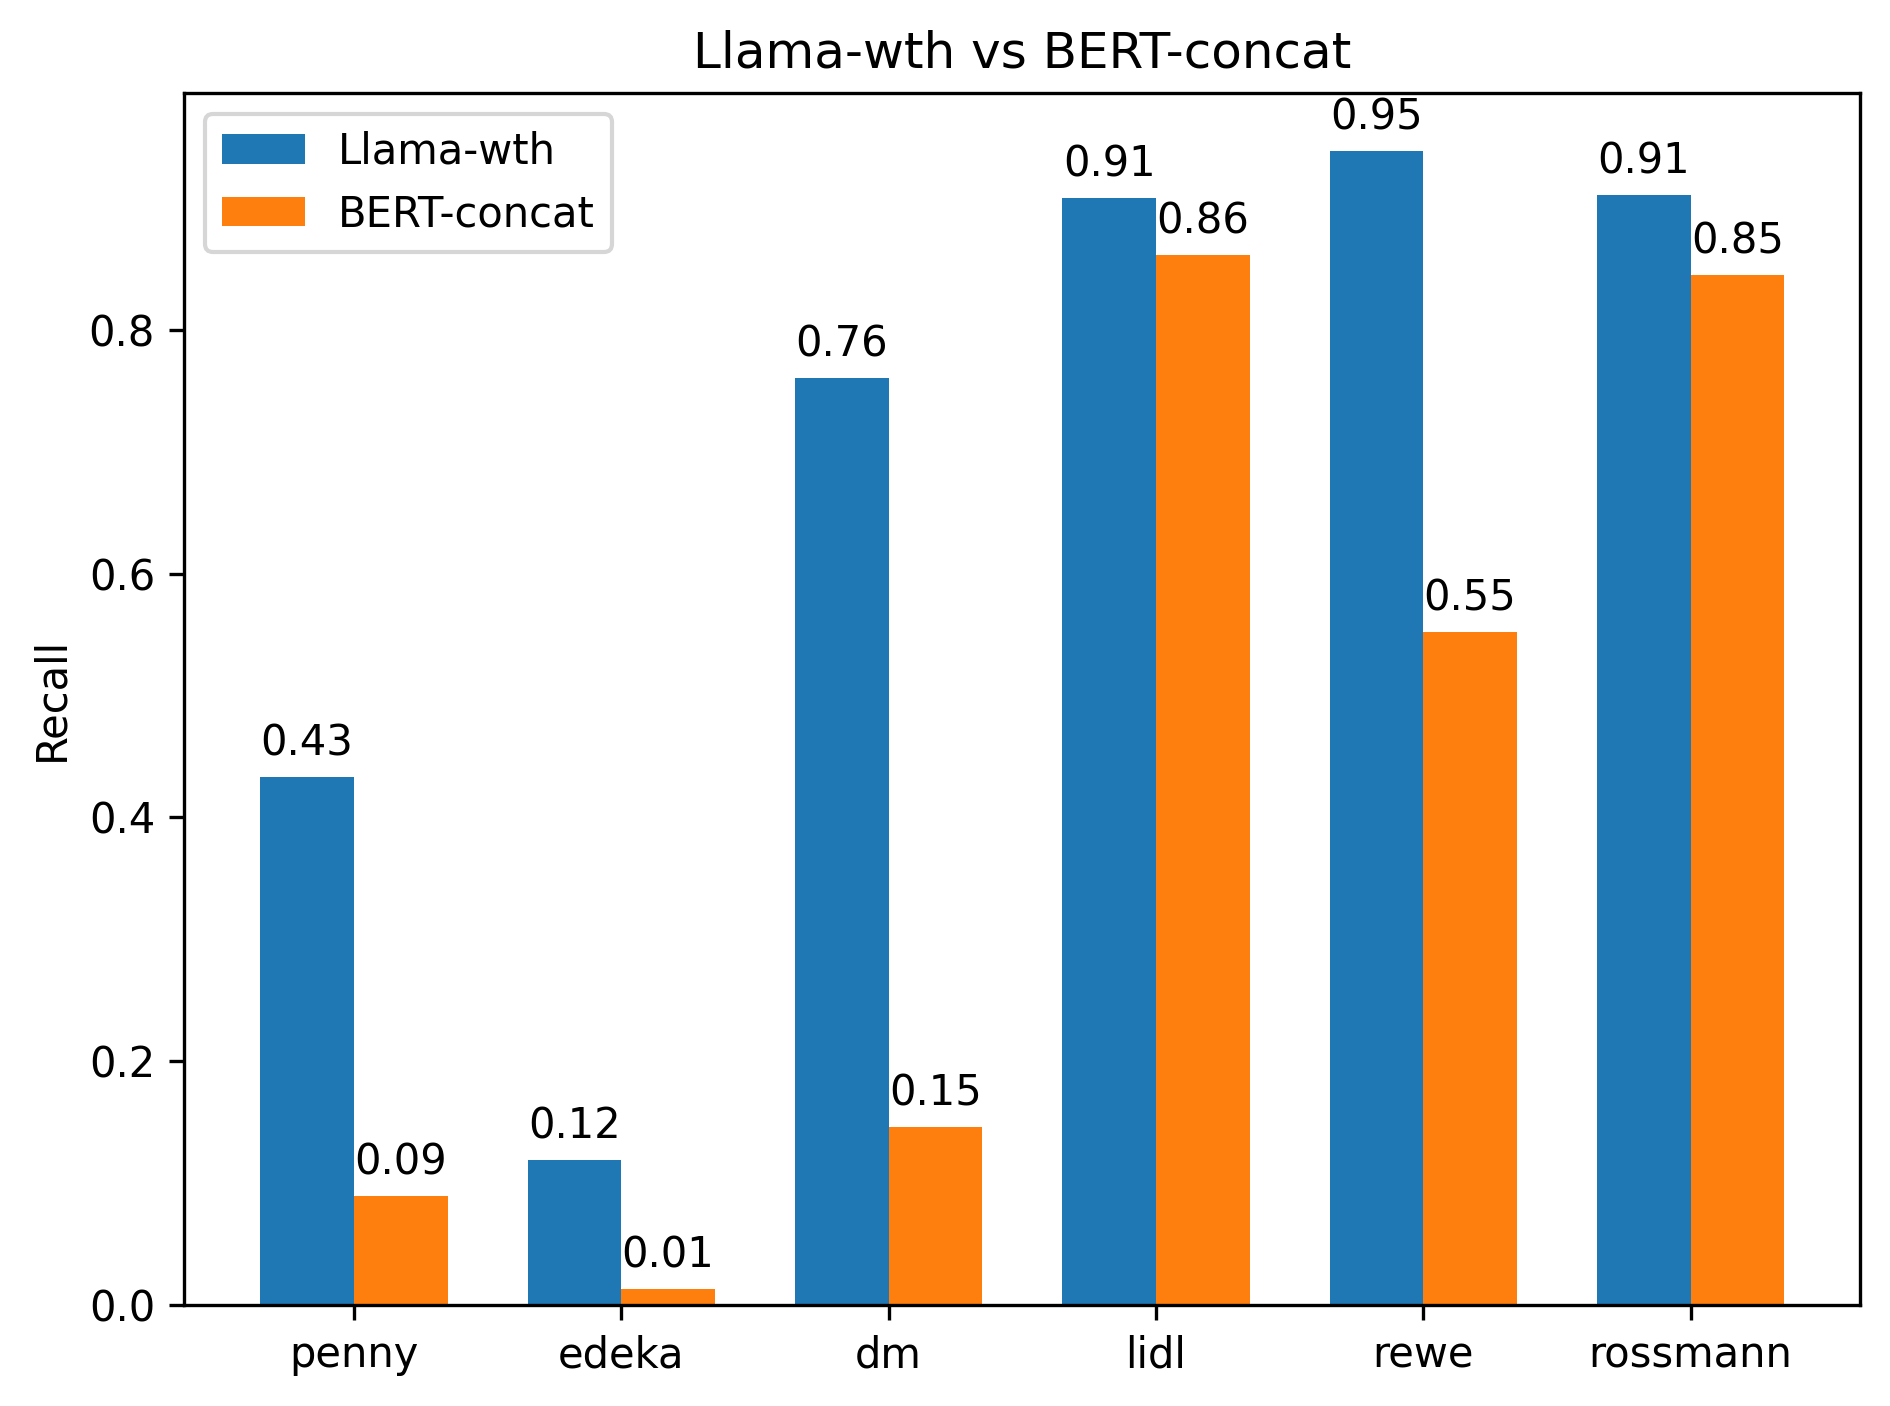
\includegraphics[width=0.8\linewidth]{bachelor_images/benchmark/llama_vs_bert_recall.png}
    \caption{Llama-wth vs BERT-concat - recall}
    \label{fig:llama_vs_bert_recall}
\end{figure}

\begin{figure}[ht]
    \centering
    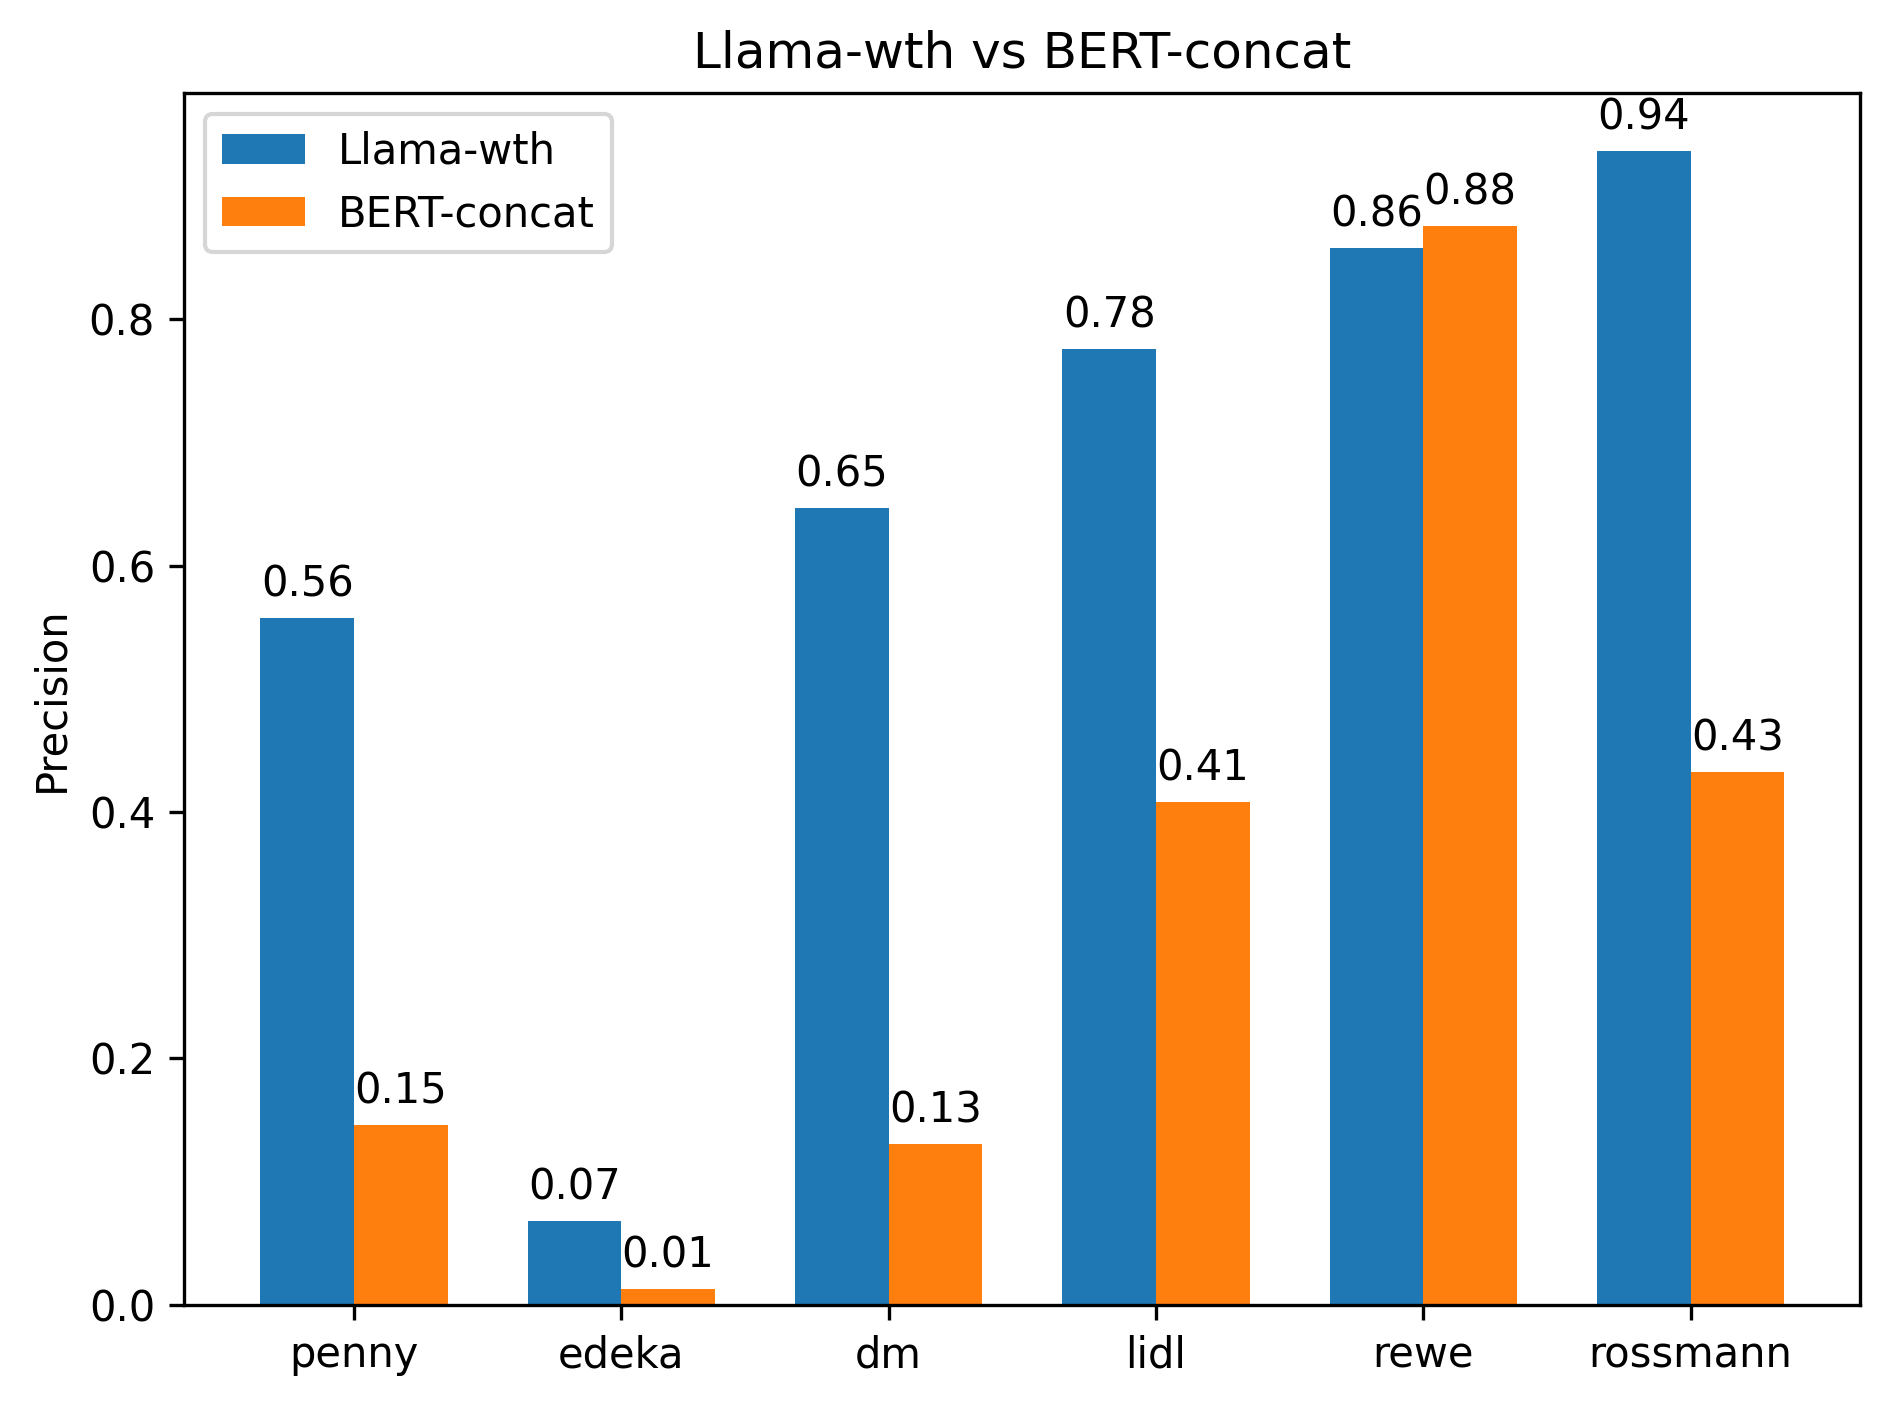
\includegraphics[width=0.8\linewidth]{bachelor_images/benchmark/llama_vs_bert_precision.png}
    \caption{Llama-wth vs BERT-concat - precision}
    \label{fig:llama_vs_bert_precision}
\end{figure}

\chapter{Llama Quantization Comparison Plots} \label{app:quant_comp}
\begin{figure}[ht]
    \centering
    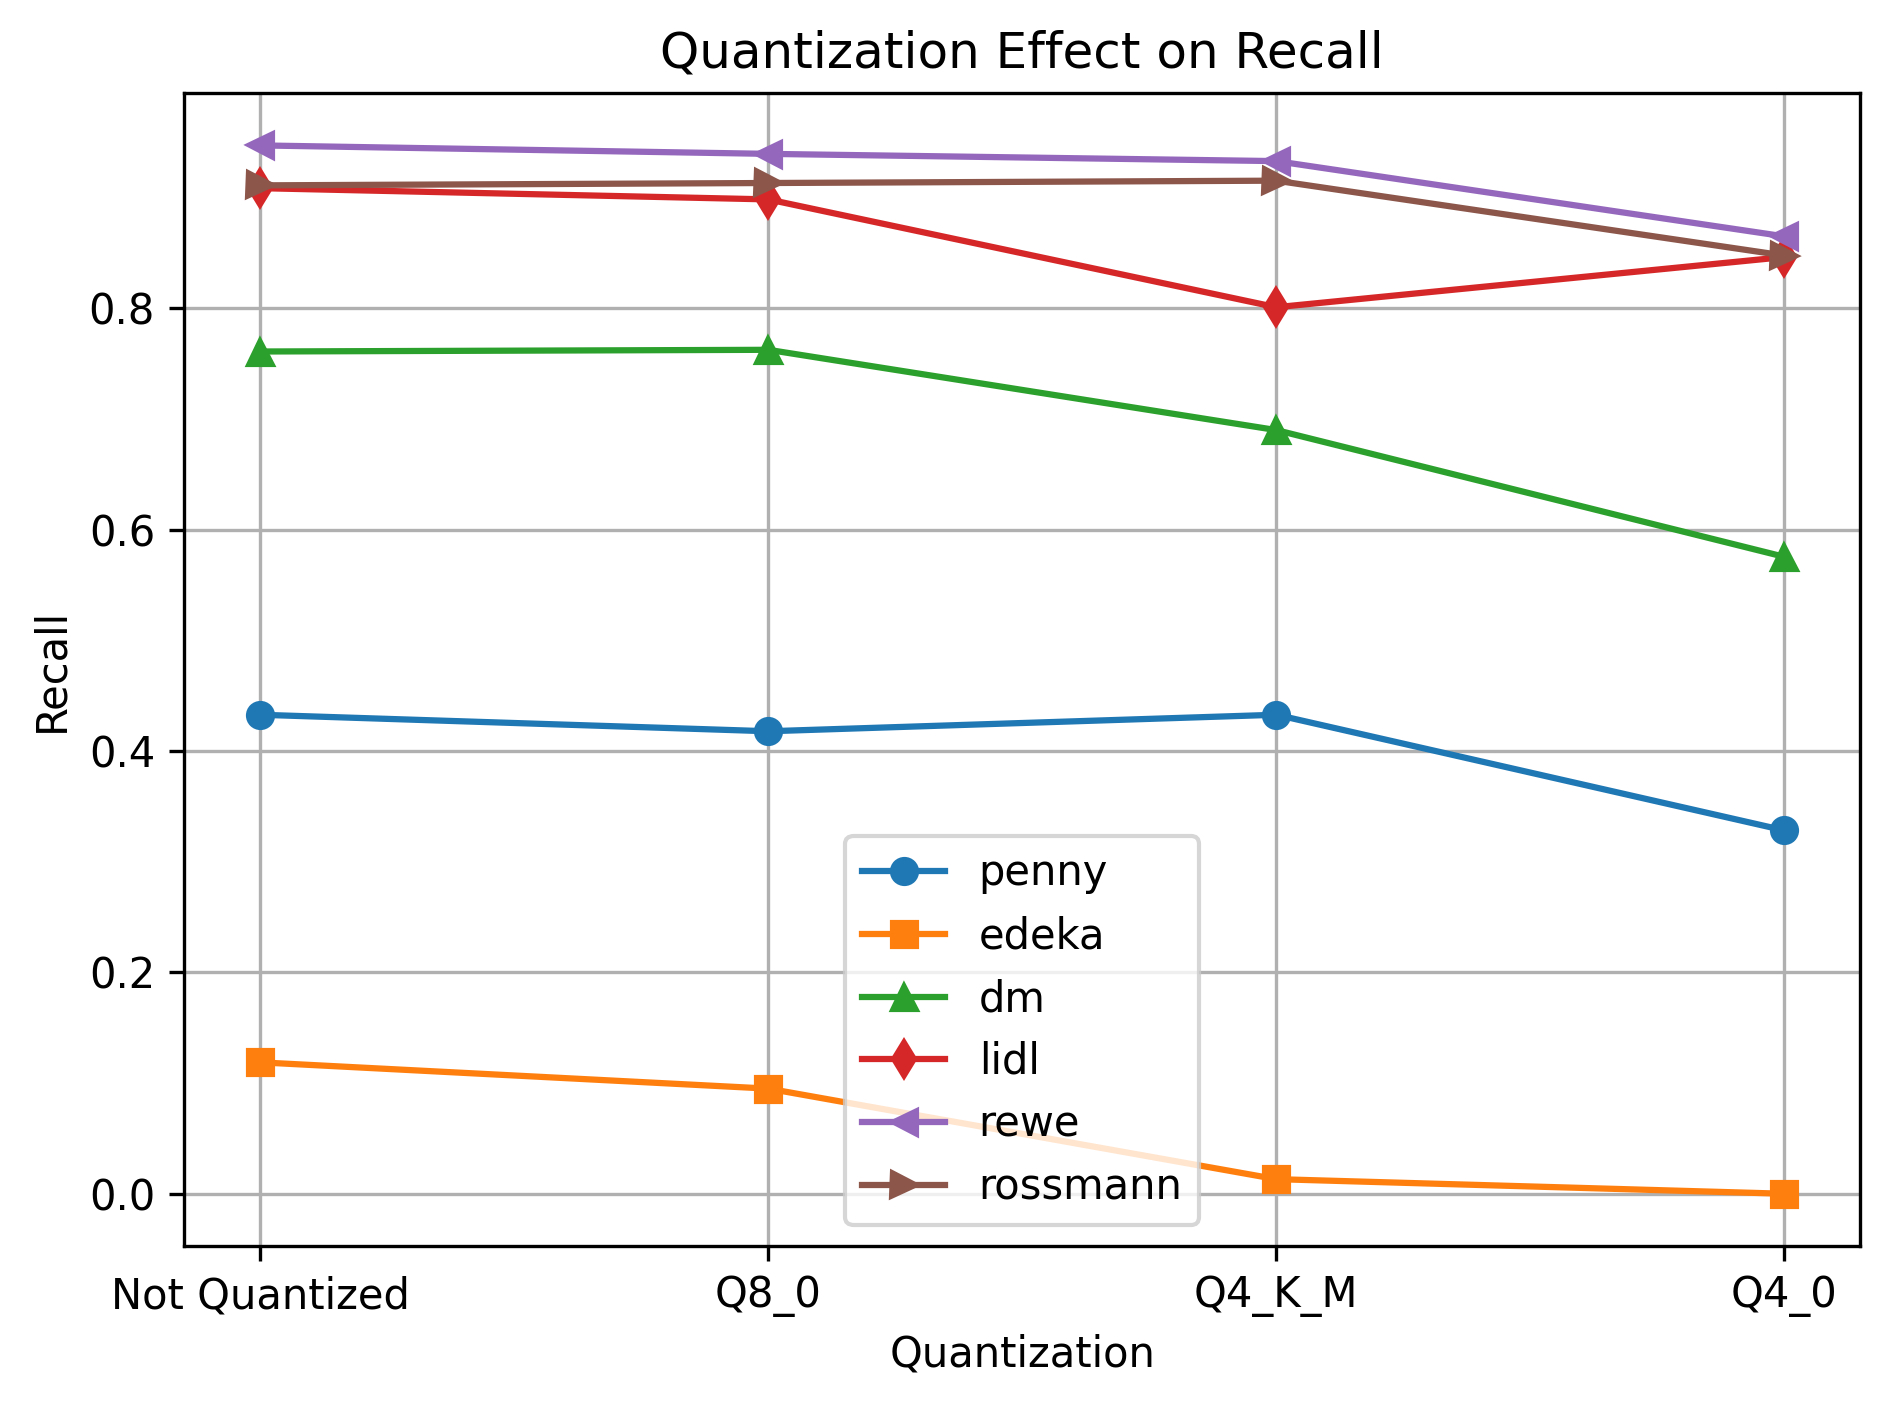
\includegraphics[width=0.8\linewidth]{bachelor_images/quant_comp/quantization_effect_on_recall.png}
    \caption{Llama-wth quantization effect on recall}
    \label{fig:quantization_effect_on_recall}
\end{figure}

\begin{figure}[ht]
    \centering
    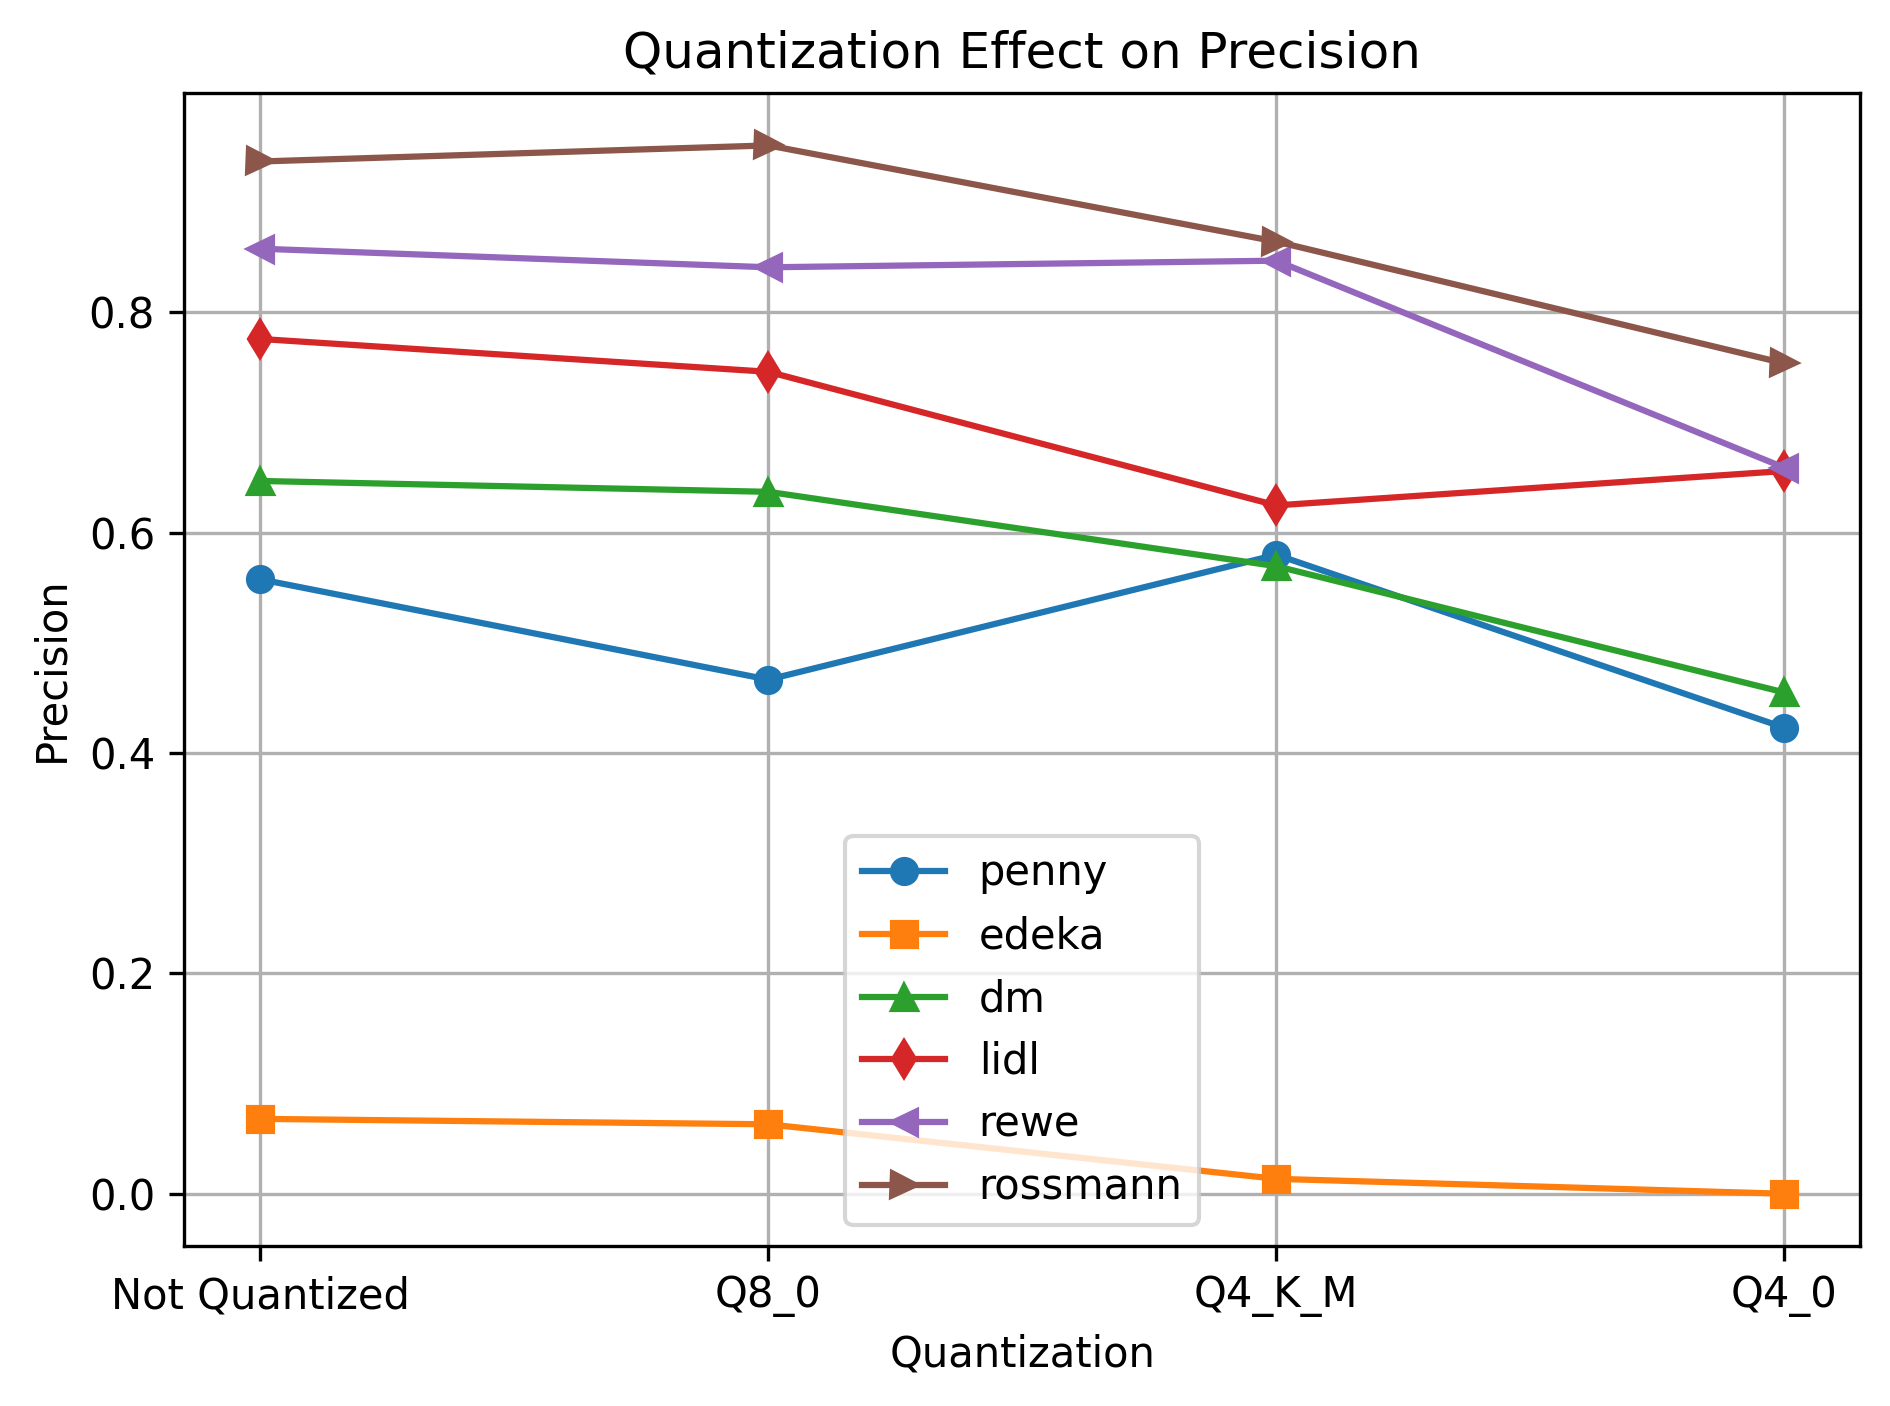
\includegraphics[width=0.8\linewidth]{bachelor_images/quant_comp/quantization_effect_on_precision.png}
    \caption{Llama-wth quantization effect on precision}
    \label{fig:quantization_effect_on_precision}
\end{figure}

\begin{figure}[ht]
    \centering
    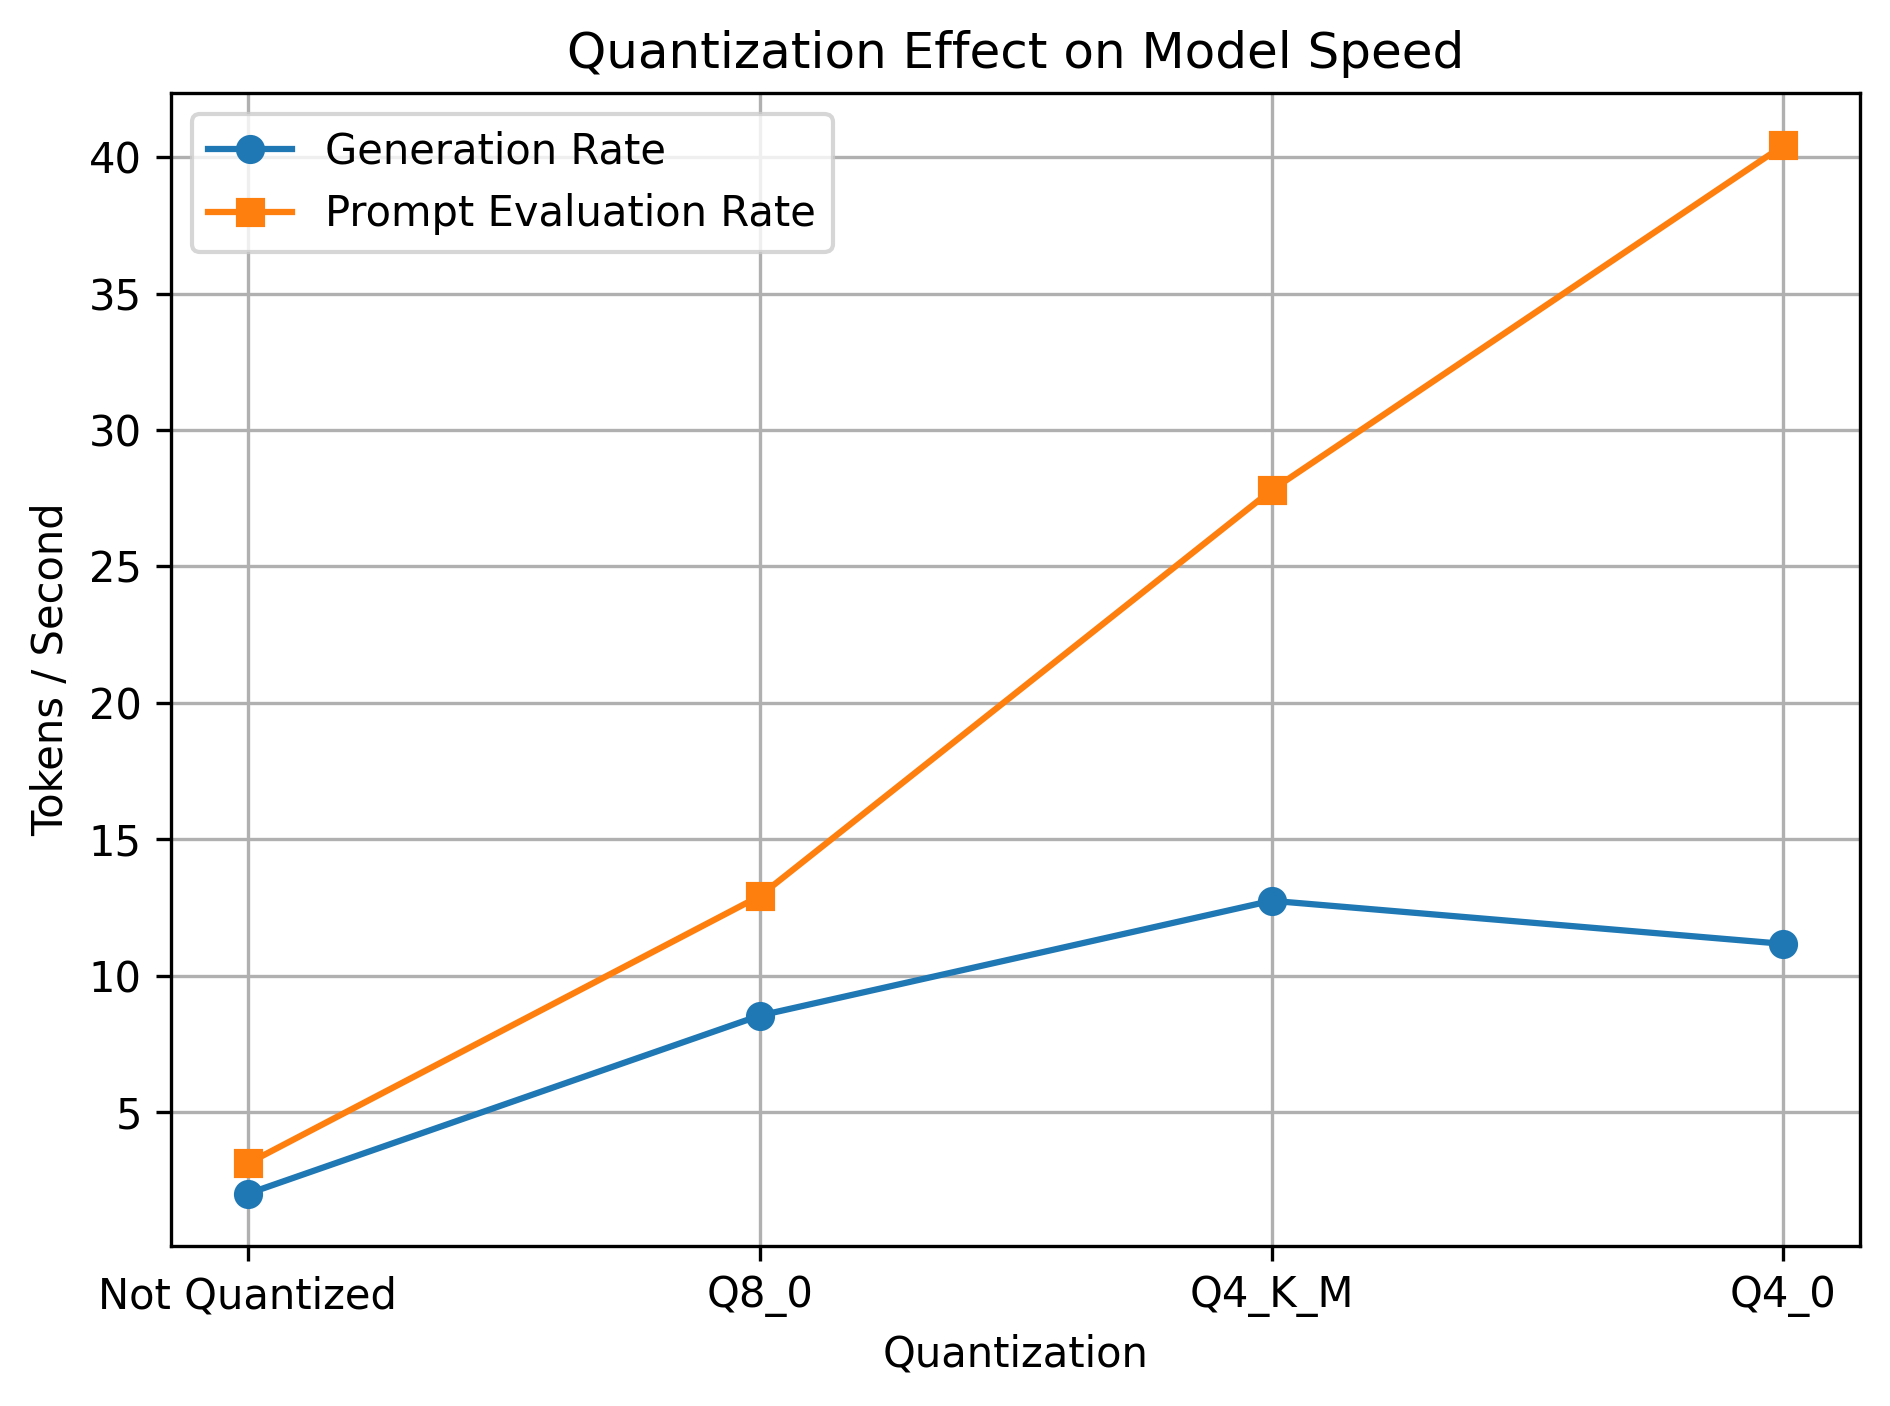
\includegraphics[width=0.8\linewidth]{bachelor_images/quant_comp/quantization_effect_on_model_speed.png}
    \caption{Llama-wth quantization effect on model speed}
    \label{fig:quantization_effect_on_model_speed}
\end{figure}

\begin{figure}[ht]
    \centering
    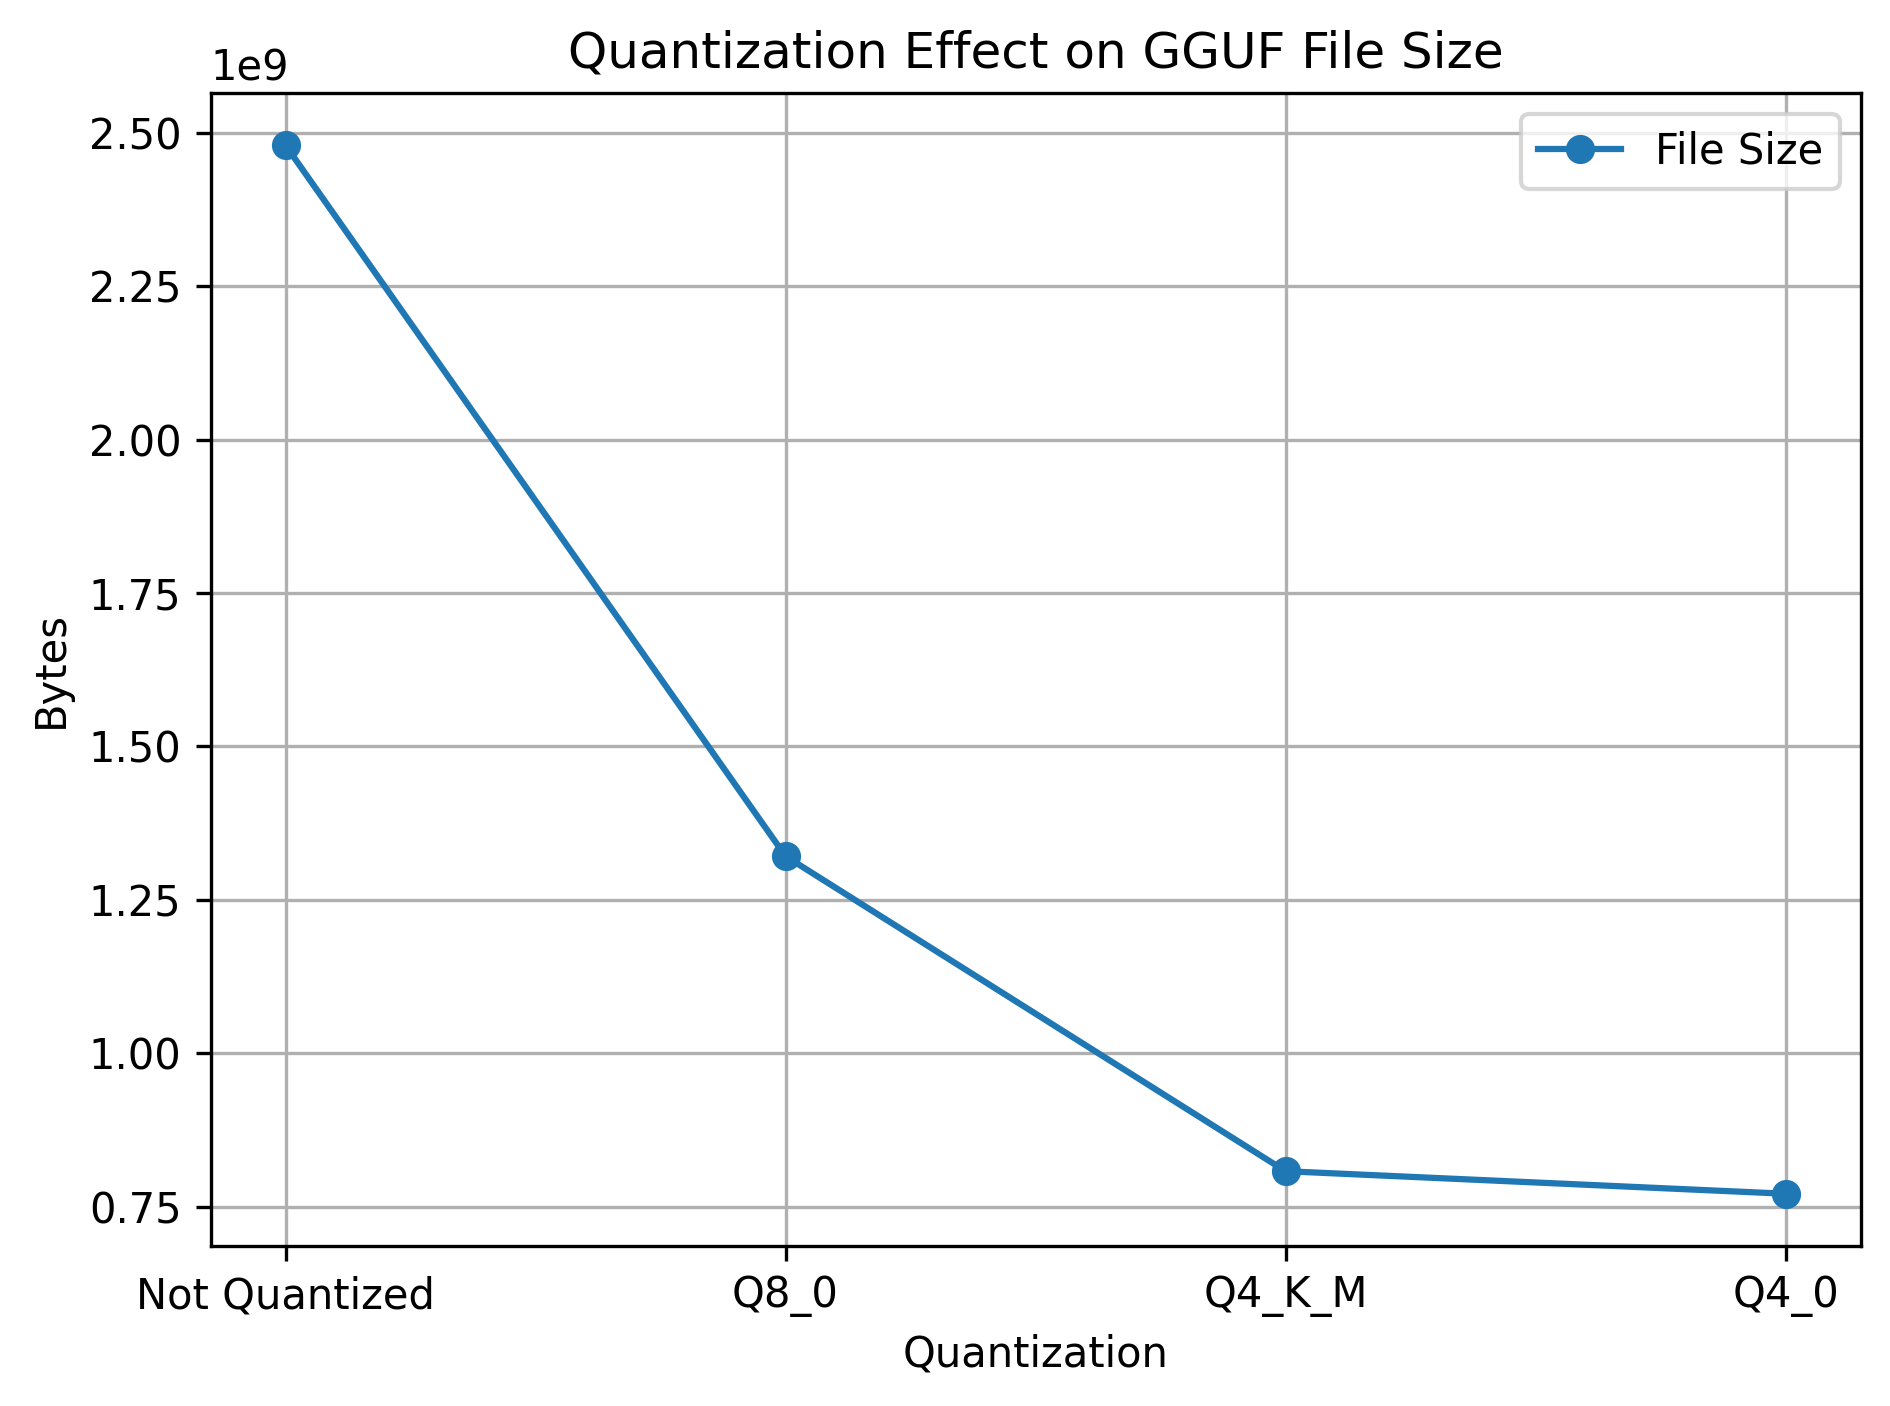
\includegraphics[width=0.8\linewidth]{bachelor_images/quant_comp/quantization_effect_on_gguf_file_size.png}
    \caption{Llama-wth quantization effect on GGUF file size}
    \label{fig:quantization_effect_on_gguf_file_size}
\end{figure}

\chapter{Llama finetuning plots} \label{AppH}
Note that the epoch numbering starts from 0. That means the leftmost value on the plots is the value after the first epoch.
In case of incremental fine-tunings, the series name indicates the source of the data in increment that was added recently.
\begin{figure}[ht]
    \centering
    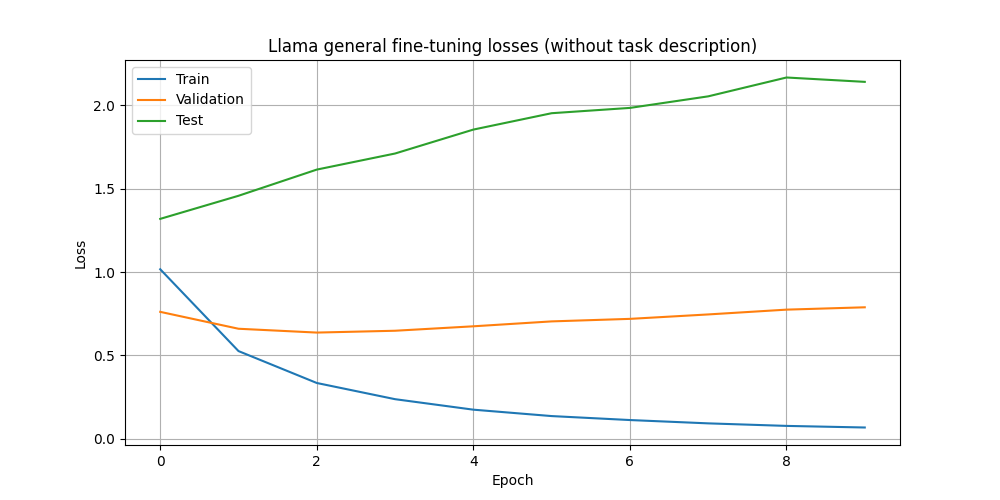
\includegraphics[width=0.8\linewidth]{bachelor_images/llama_ft/llama-wth-loss.png}
    \caption{Llama fine-tuning losses for baseline experiment.}
    \label{fig:llama-wth-loss}
\end{figure}
\begin{figure}[ht]
    \centering
    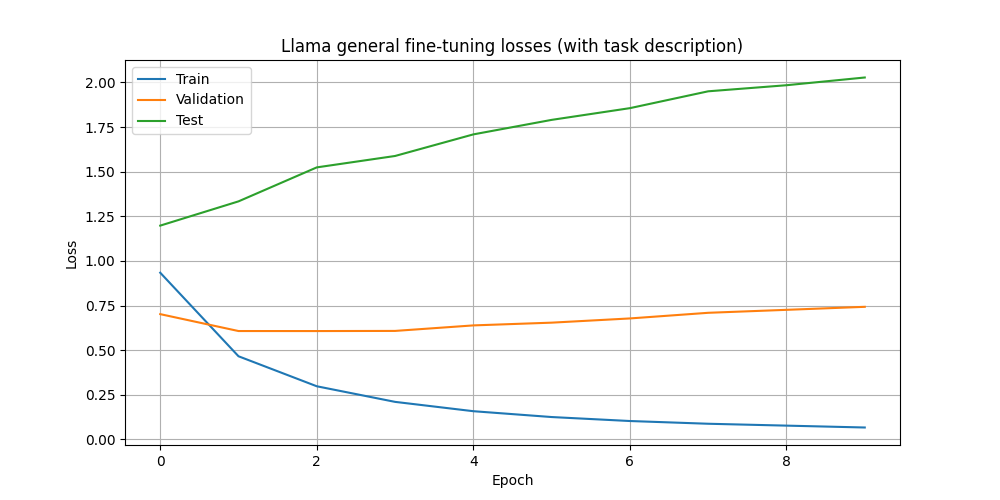
\includegraphics[width=0.8\linewidth]{bachelor_images/llama_ft/llama-w-loss.png}
    \caption{Llama fine-tuning losses for baseline experiment (with task description).}
    \label{fig:llama-w-loss}
\end{figure}
\begin{figure}[ht]
    \centering
    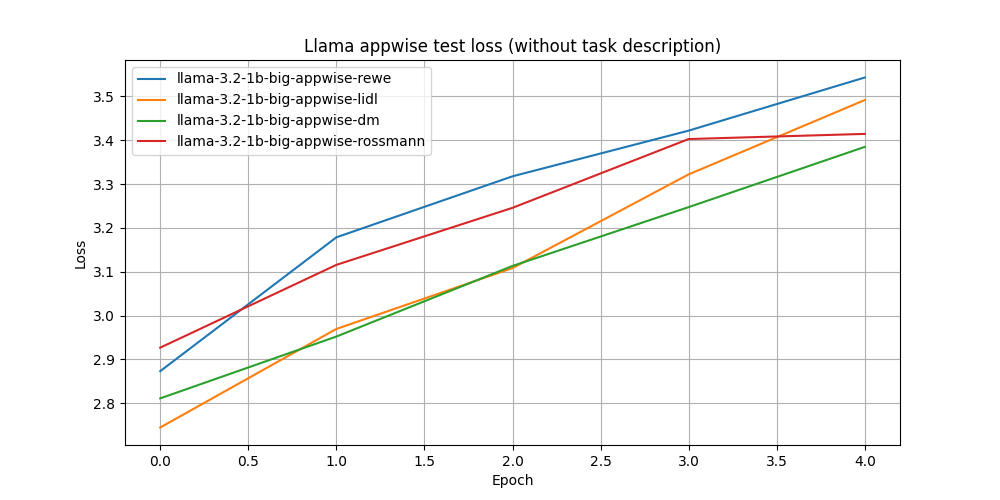
\includegraphics[width=0.8\linewidth]{bachelor_images/llama_ft/llama-appwise-wth-test.png}
    \caption{Llama fine-tuning test losses for application-wise runs.}
    \label{fig:llama-wth-appwise}
\end{figure}
\begin{figure}[ht]
    \centering
    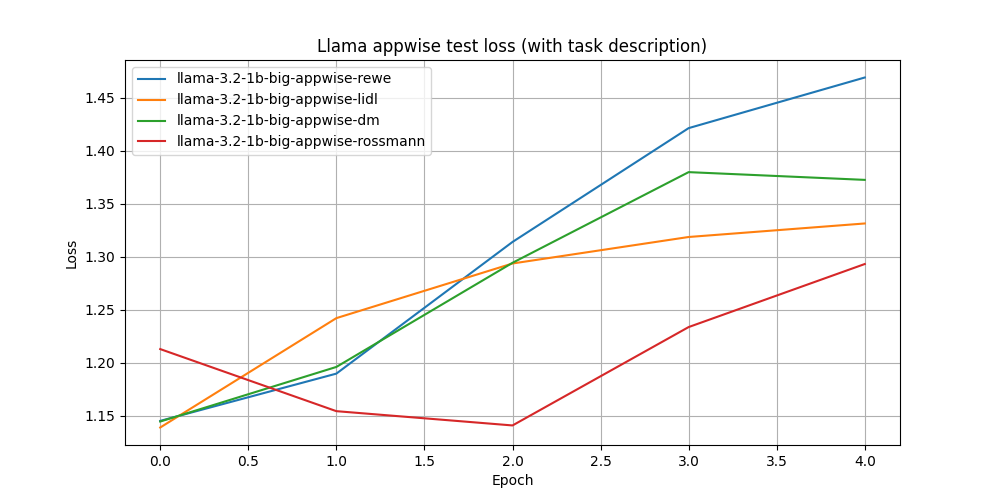
\includegraphics[width=0.8\linewidth]{bachelor_images/llama_ft/llama-appwise-w-test.png}
    \caption{Llama fine-tuning test losses for application-wise runs (with task description).}
    \label{fig:llama-w-appwise}
\end{figure}
\begin{figure}[ht]
    \centering
    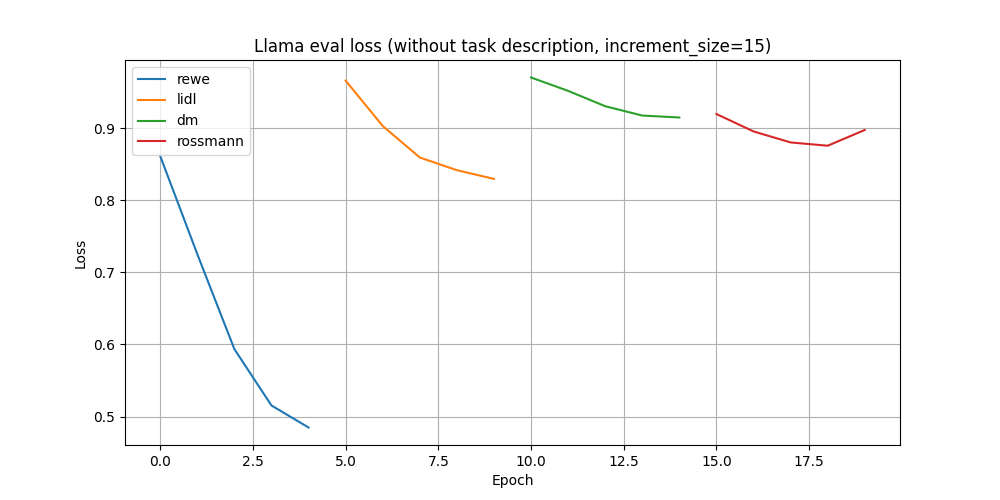
\includegraphics[width=0.8\linewidth]{bachelor_images/llama_ft/llama-inc-15-tot-eval.png}
    \caption{Llama evaluation loss for fine-tuning with concatenated increments of size 15.}
    \label{fig:llama-inc-tot-15-eval}
\end{figure}
\begin{figure}[ht]
    \centering
    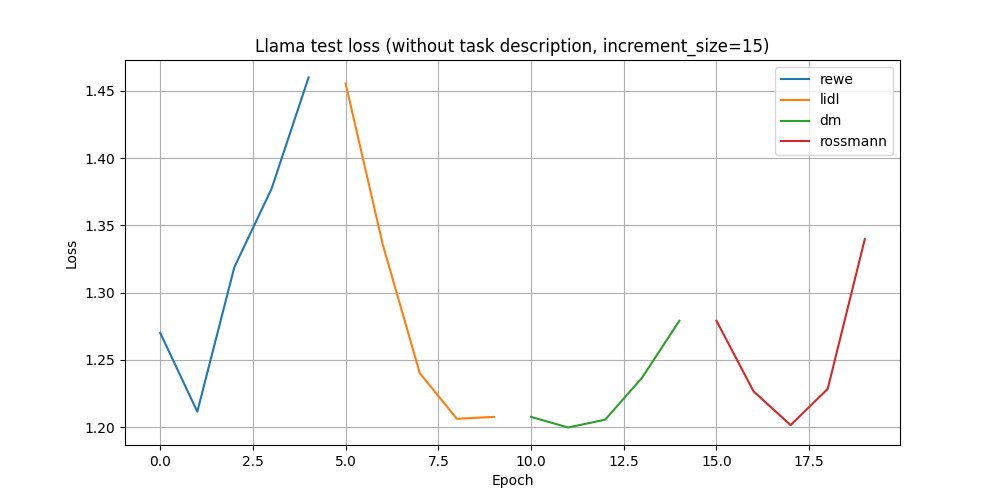
\includegraphics[width=0.8\linewidth]{bachelor_images/llama_ft/llama-inc-15-tot-test.png}
    \caption{Llama test loss for fine-tuning with concatenated increments of size 15.}
    \label{fig:llama-inc-tot-15-test}
\end{figure}
\begin{figure}[ht]
    \centering
    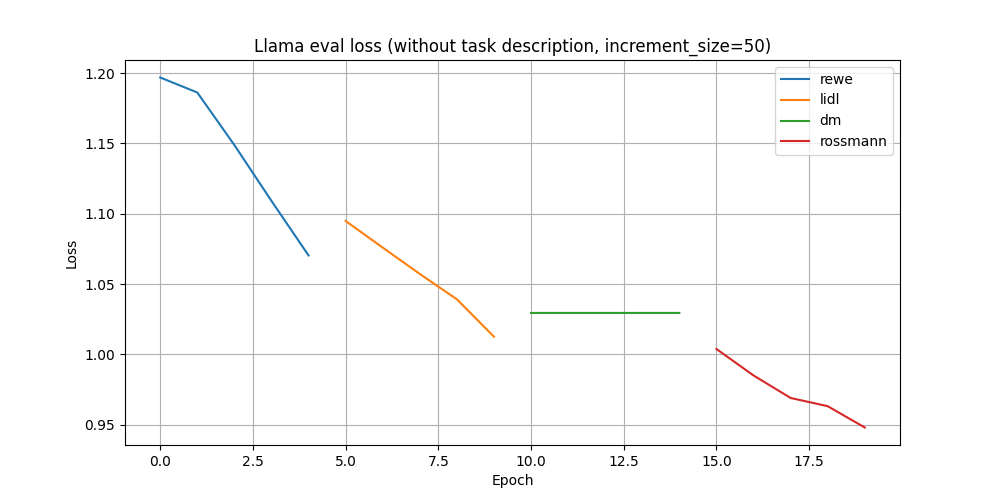
\includegraphics[width=0.8\linewidth]{bachelor_images/llama_ft/llama-inc-50-tot-eval.png}
    \caption{Llama evaluation loss for fine-tuning with concatenated increments of size 50.}
    \label{fig:llama-inc-tot-50-eval}
\end{figure}
\begin{figure}[ht]
    \centering
    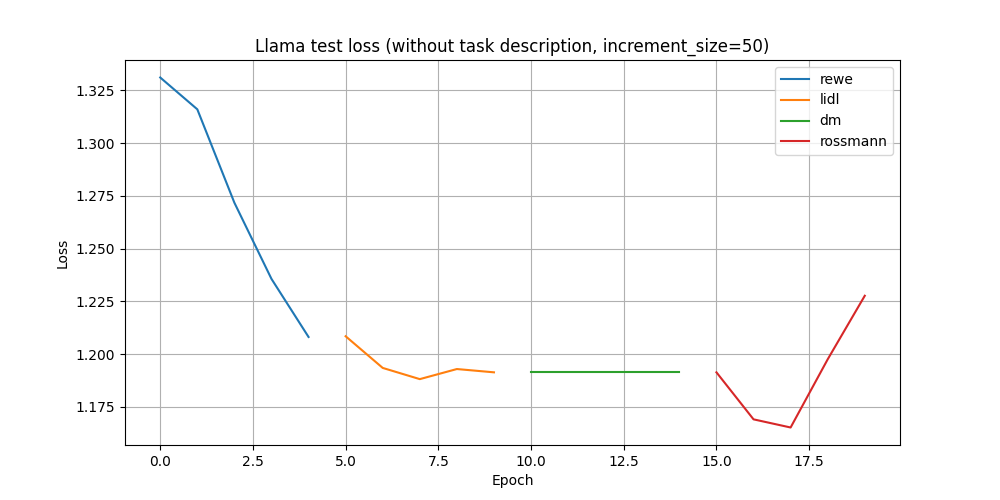
\includegraphics[width=0.8\linewidth]{bachelor_images/llama_ft/llama-inc-50-tot-test.png}
    \caption{Llama test loss for fine-tuning with concatenated increments of size 50.}
    \label{fig:llama-inc-tot-50-test}
\end{figure}
\begin{figure}[ht]
    \centering
    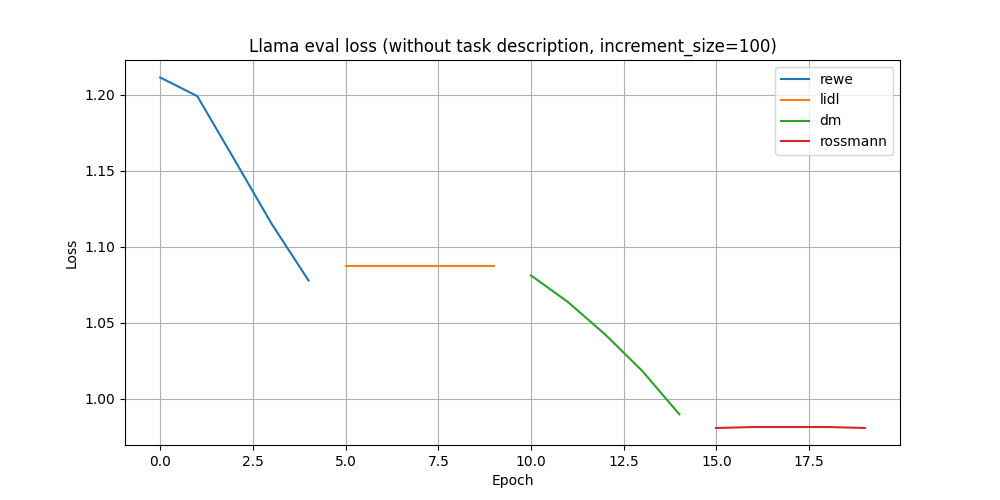
\includegraphics[width=0.8\linewidth]{bachelor_images/llama_ft/llama-inc-100-tot-eval.png}
    \caption{Llama evaluation loss for fine-tuning with concatenated increments of size 100.}
    \label{fig:llama-inc-tot-100-eval}
\end{figure}
\begin{figure}[ht]
    \centering
    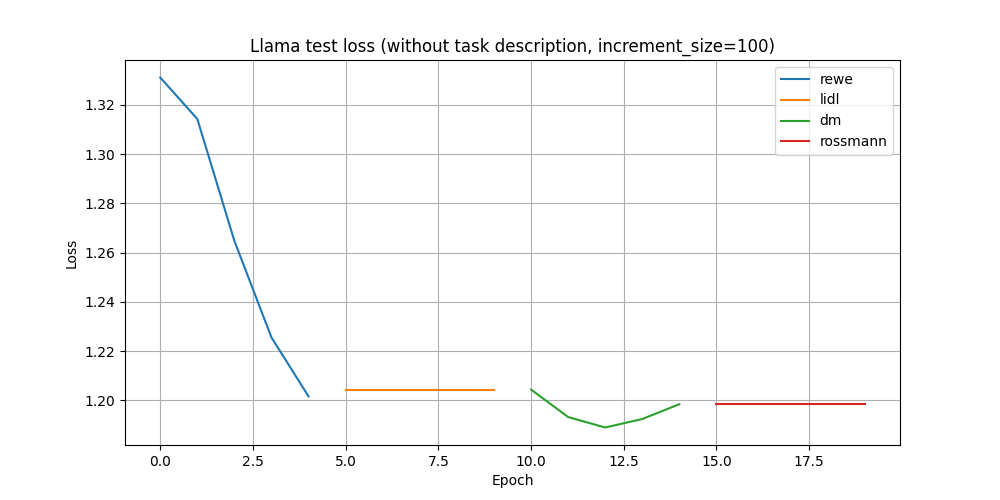
\includegraphics[width=0.8\linewidth]{bachelor_images/llama_ft/llama-inc-100-tot-test.png}
    \caption{Llama test loss for fine-tuning with concatenated increments of size 100.}
    \label{fig:llama-inc-tot-100-test}
\end{figure}


\begin{figure}[ht]
    \centering
    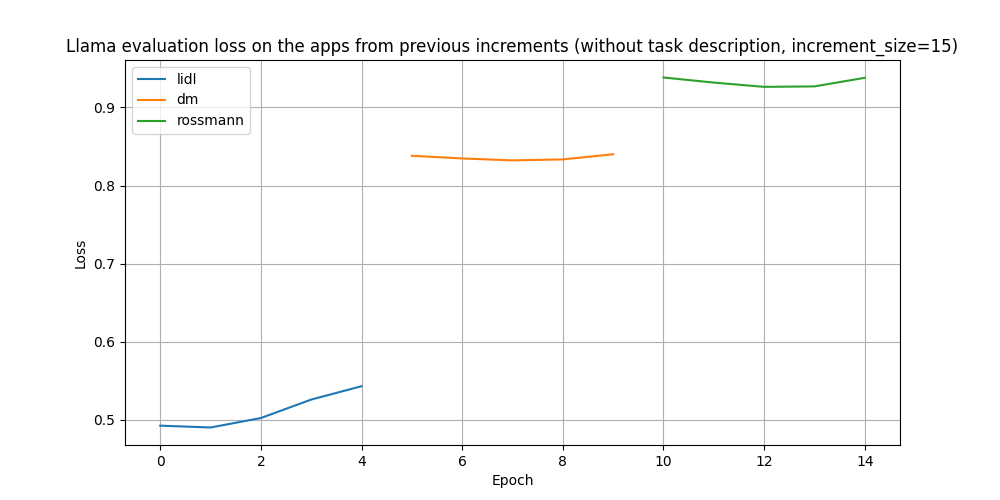
\includegraphics[width=0.8\linewidth]{bachelor_images/llama_ft/llama-inc-15-eval-prev.png}
    \caption{Llama evaluation loss for previous increments for fine-tuning with increments of size 15.}
    \label{fig:llama-inc-15-eval}
\end{figure}
\begin{figure}[ht]
    \centering
    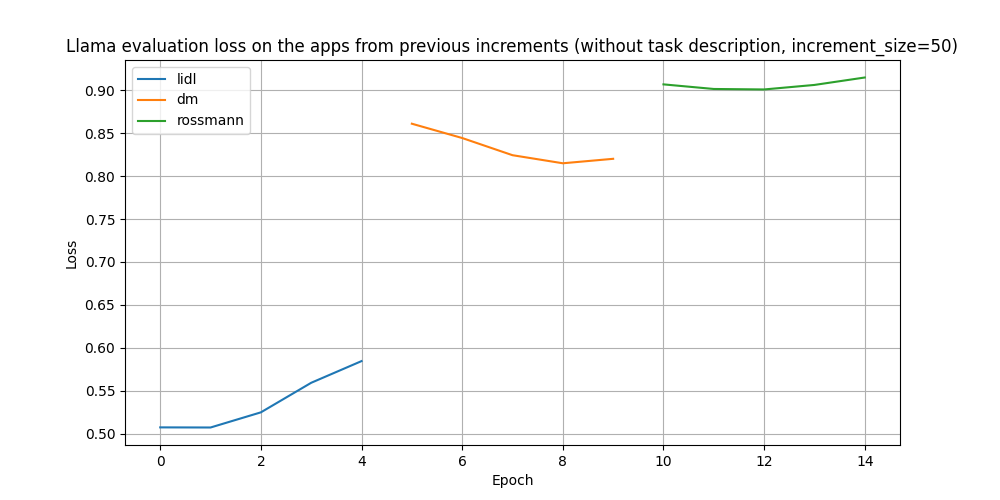
\includegraphics[width=0.8\linewidth]{bachelor_images/llama_ft/llama-inc-50-eval-prev.png}
    \caption{Llama evaluation loss for previous increments for fine-tuning with increments of size 50.}
    \label{fig:llama-inc-50-eval}
\end{figure}
\begin{figure}[ht]
    \centering
    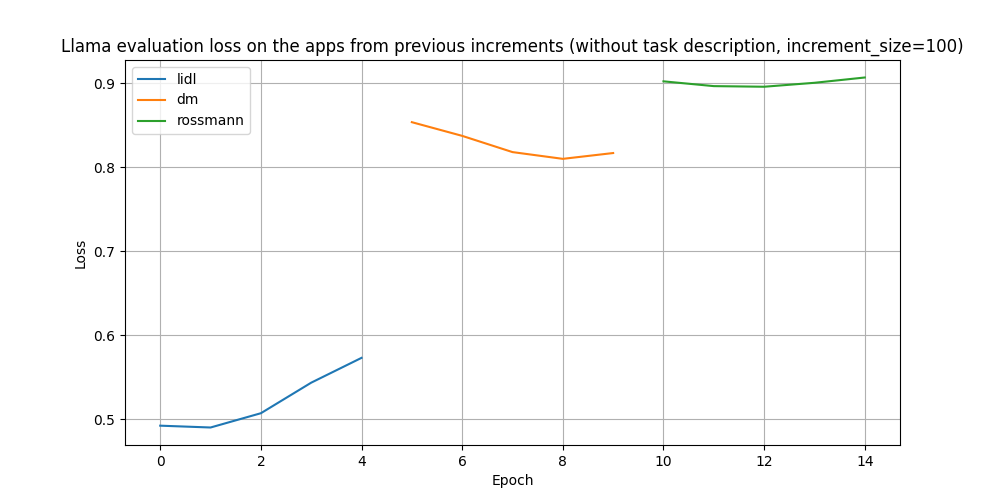
\includegraphics[width=0.8\linewidth]{bachelor_images/llama_ft/llama-inc-100-eval-prev.png}
    \caption{Llama evaluation loss for previous increments for fine-tuning with increments of size 100.}
    \label{fig:llama-inc-100-eval}
\end{figure}
\begin{figure}[ht]
    \centering
    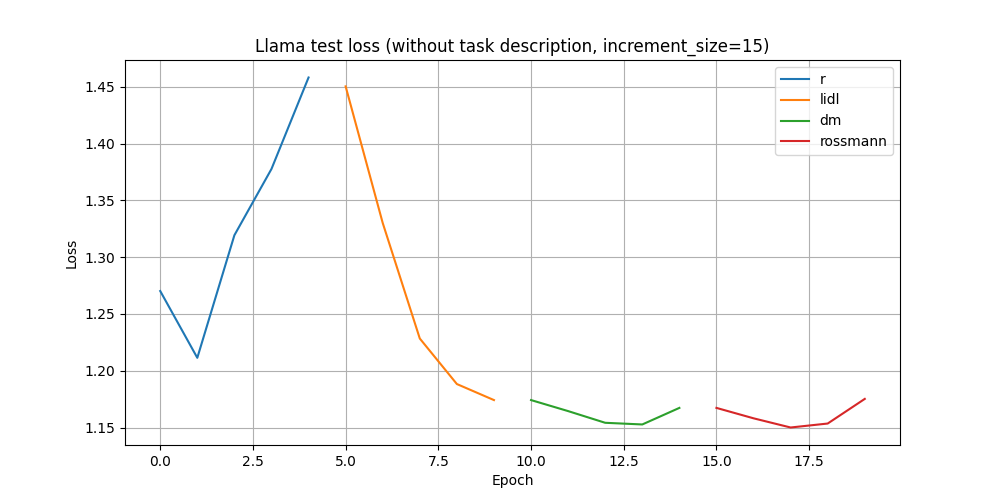
\includegraphics[width=0.8\linewidth]{bachelor_images/llama_ft/llama-inc-15-test.png}
    \caption{Llama test loss for fine-tuning with increments of size 15.}
    \label{fig:llama-inc-15-test}
\end{figure}
\begin{figure}[ht]
    \centering
    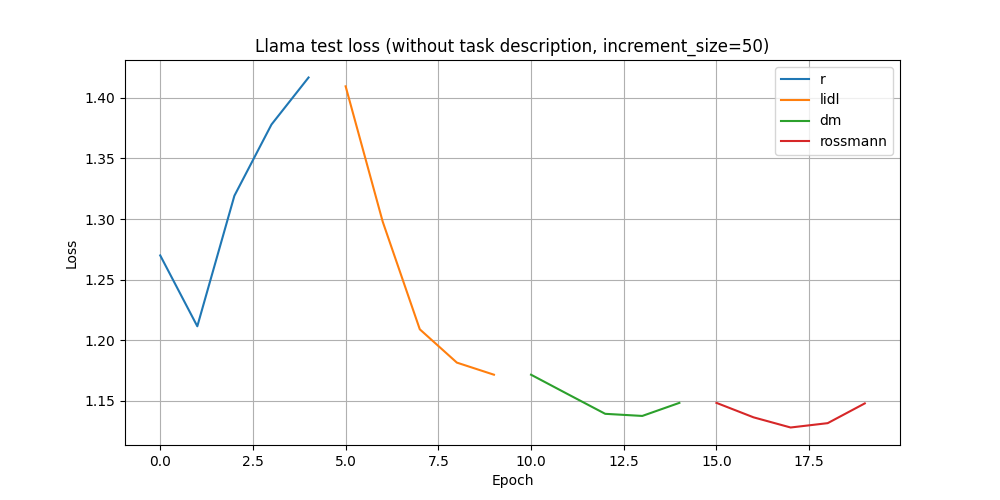
\includegraphics[width=0.8\linewidth]{bachelor_images/llama_ft/llama-inc-50-test.png}
    \caption{Llama test loss for fine-tuning with increments of size 50.}
    \label{fig:llama-inc-50-test}
\end{figure}
\begin{figure}[ht]
    \centering
    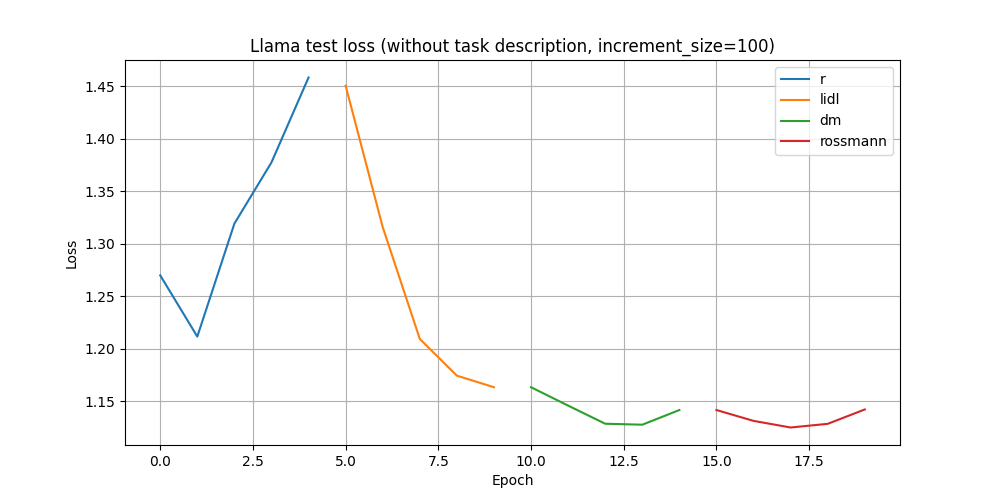
\includegraphics[width=0.8\linewidth]{bachelor_images/llama_ft/llama-inc-100-test.png}
    \caption{Llama test loss for fine-tuning with increments of size 100.}
    \label{fig:llama-inc-100-test}
\end{figure}

\begin{figure}[ht]
    \centering
    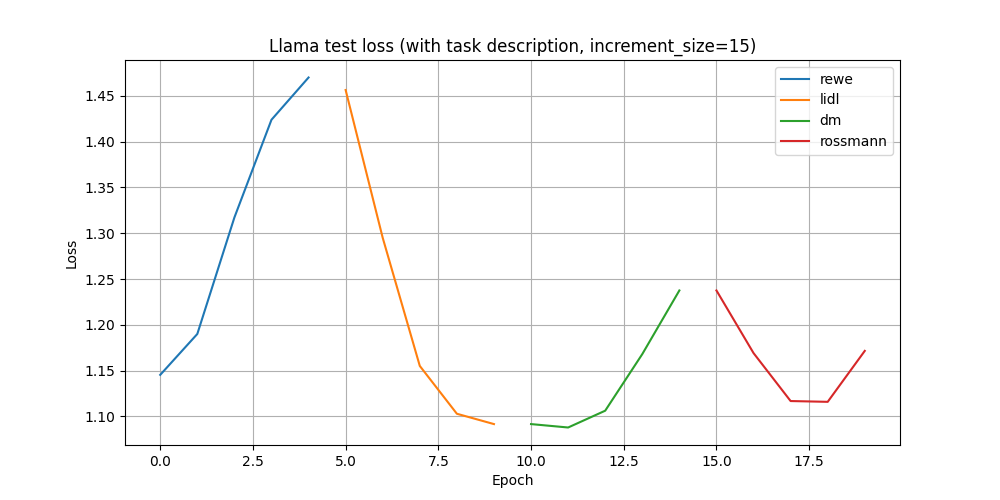
\includegraphics[width=0.8\linewidth]{bachelor_images/llama_ft/llama-inc-15-tot-test-w.png}
    \caption{Llama test loss for fine-tuning with concatenated increments of size 15.}
    \label{fig:llama-inc-tot-15-test-w}
\end{figure}
\begin{figure}[ht]
    \centering
    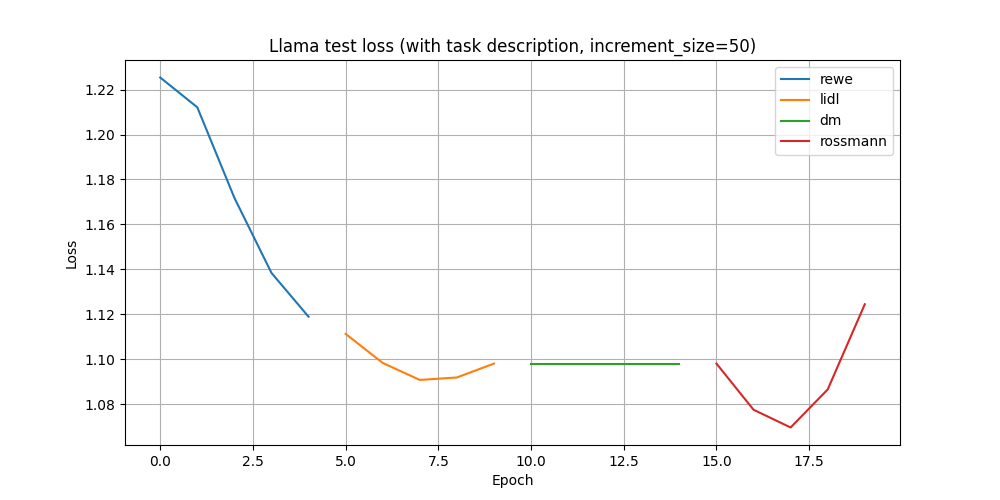
\includegraphics[width=0.8\linewidth]{bachelor_images/llama_ft/llama-inc-50-tot-test-w.png}
    \caption{Llama test loss for fine-tuning with concatenated increments of size 50.}
    \label{fig:llama-inc-tot-50-test-w}
\end{figure}
\begin{figure}[ht]
    \centering
    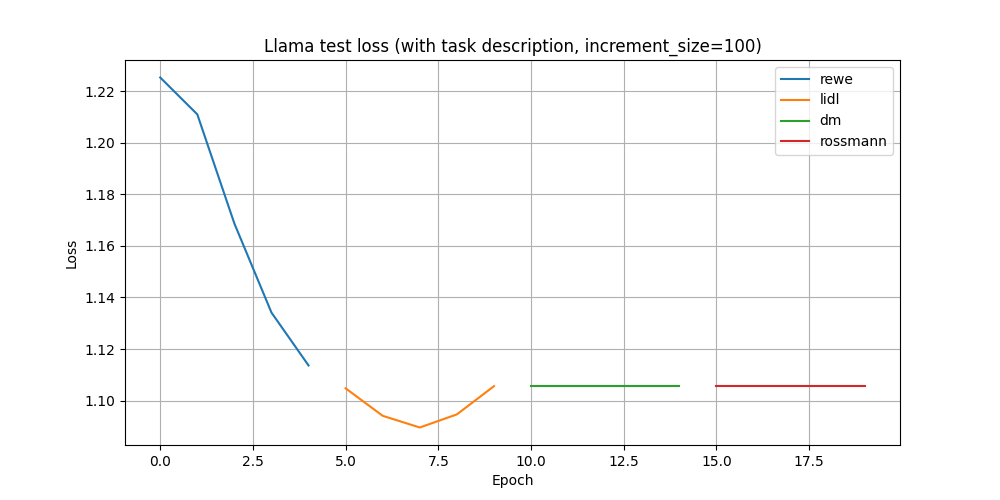
\includegraphics[width=0.8\linewidth]{bachelor_images/llama_ft/llama-inc-100-tot-test-w.png}
    \caption{Llama test loss for fine-tuning with concatenated increments of size 100.}
    \label{fig:llama-inc-tot-100-test-w}
\end{figure}
\begin{figure}[ht]
    \centering
    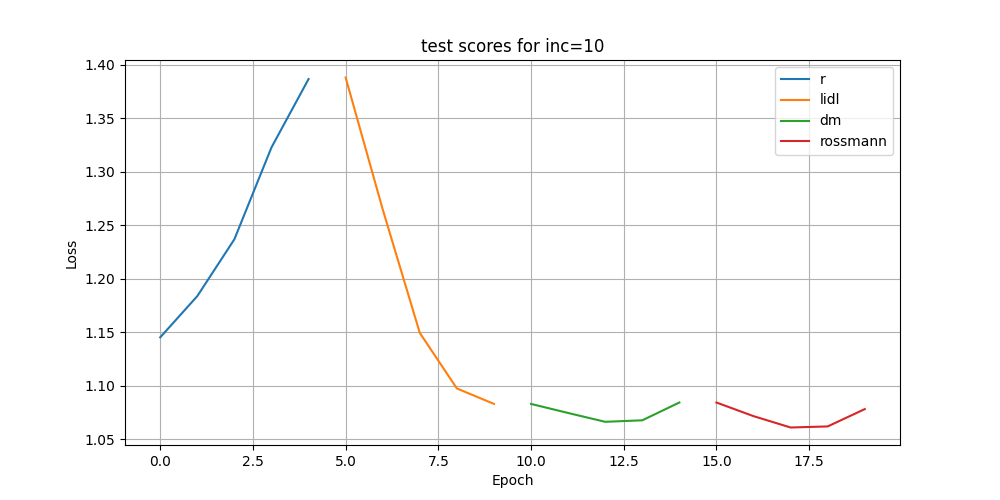
\includegraphics[width=0.8\linewidth]{bachelor_images/llama_ft/llama-inc-10-test-w.png}
    \caption{Llama test loss for fine-tuning with increments of size 10.}
    \label{fig:llama-inc-10-test-w}
\end{figure}
\begin{figure}[ht]
    \centering
    \includegraphics[width=0.8\linewidth]{bachelor_images/llama_ft/llama-inc-50-test-w.png}
    \caption{Llama test loss for fine-tuning with increments of size 50.}
    \label{fig:llama-inc-50-test-w}
\end{figure}
\begin{figure}[ht]
    \centering
    \includegraphics[width=0.8\linewidth]{bachelor_images/llama_ft/llama-inc-100-test-w.png}
    \caption{Llama test loss for fine-tuning with increments of size 100.}
    \label{fig:llama-inc-100-test-w}
\end{figure}

\end{appendices}

% \chapter{Technologies}
% \chapter{Architecture design}
% \chapter{Pipelines}
% \chapter{Benchmark}
% \chapter{Performance}
% \chapter{Possible extensions}
% \chapter{Conclusion}
% \chapter{Charts}

\begin{thebibliography}{99}

\addcontentsline{toc}{chapter}{Bibliography}
\raggedright

\bibitem{murmuras} 
\textit{Murmuras website}.  
\url{https://murmuras.com/}.  
[Accessed 2025-02-11].

\bibitem{seo2023}
\textit{Seo, D., \& Yoo, Y. (2023). Improving Shopping Mall Revenue by Real-Time Customized Digital Coupon Issuance. IEEE Access, 11, 7924–7932.}
\url{https://doi.org/10.1109/ACCESS.2023.3239425}

\bibitem{coupon_definition}
\textit{Britannica Dictionary definition of COUPON}.
\url{https://www.britannica.com/dictionary/coupon}.
[Accessed 2025-02-03].

\bibitem{nayal2021}
\textit{Nayal, P., \& Pandey, N. (2021). What Makes a Consumer Redeem Digital Coupons? Behavioral Insights from Grounded Theory Approach. *Journal of Promotion Management*, 28(3), 205–238.}
\url{https://doi.org/10.1080/10496491.2021.1989541}

\bibitem{danaher2015}
\textit{Danaher, P. J., Smith, M. S., Ranasinghe, K., \& Danaher, T. S. (2015). *Where, when, and how long: Factors that influence the redemption of mobile phone coupons.* *Journal of Marketing Research*, *52*(5), 710--725.}
\url{https://journals.sagepub.com/doi/full/10.1509/jmr.13.0341}

\bibitem{jayadharshini2023}
\textit{Jayadharshini, P., Sharon Roji, Priya. C, Lalitha, K., Santhiya, S., Keerthika, S., \& Abinaya, N. (2023). *Enhancing Retailer Auctions and Analyzing the Impact of Coupon Offers on Customer Engagement and Sales Through Machine Learning.* *2023 Intelligent Computing and Control for Engineering and Business Systems (ICCEBS)*, 1–6. }
\url{https://doi.org/10.1109/ICCEBS58601.2023.10448900}

\bibitem{design_of_coupons}
Xiong Keyi, Yang Wensheng
\textit{Research on the Design of E-coupons for Directional Marketing of Two Businesses in Competitive Environment}.
\url{https://www.sciencepublishinggroup.com/article/10.11648/j.ijefm.20200801.16}.
[Accessed 2025-02-04].

\bibitem{li2024}
\textit{Li, J. (2024). The evolution, applications, and future prospects of large language models: An in-depth overview. Applied and Computational Engineering 35, 234–244.}\url{https://doi.org/10.54254/2755-2721/35/20230399}

\bibitem{sui2024}
\textit{Sui, Y., Zhou, M., Zhou, M., Han, S., \& Zhang, D. (2024). Table meets LLM: Can large language models understand structured table data? A benchmark and empirical study. Proceedings of the 17th ACM International Conference on Web Search and Data Mining, 645--654.}

\bibitem{targeted_reminders}
Li Li, et. al.
\textit{Targeted reminders of electronic coupons: using predictive analytics to facilitate coupon marketing}.
\url{https://link.springer.com/article/10.1007/s10660-020-09405-4}.
[Accessed 2025-02-04].

\bibitem{competitor_tariffs}
Bernhard König, et. al.
\textit{Analysing competitor tariffs with machine learning}.
\url{https://www.milliman.com/en/insight/analysing-competitor-tariffs-with-machine-learning}.
[Accessed 2025-02-04].

\bibitem{ml_general}
Iqbal H. Sarker
\textit{Machine Learning: Algorithms, Real-World Applications and Research Directions}.
\url{https://link.springer.com/article/10.1007/s42979-021-00592-x}.
[Accessed 2025-02-05].

\bibitem{emarketer_coupon_stats}
Sara Lebow
\textit{How consumers access digital coupons}.
\url{https://www.emarketer.com/content/how-consumers-access-digital-coupons}.
[Accessed 2025-02-05].

\bibitem{coupon_stats_2}
\textit{Unveiling IT Coupons Trends and Statistics}
\url{https://www.go-globe.com/unveiling-it-coupons-trends-statistics/}.
[Accessed 2025-02-05].

\bibitem{android_view}
\textit{Android API Reference - View}
\url{https://developer.android.com/reference/android/view/View}
[Accessed 2025-03-11]

\bibitem{brinkmann2023}
\textit{Brinkmann, A., Shraga, R., Der, R. C., \& Bizer, C. (2023). Product Information Extraction using ChatGPT. arXiv preprint, arXiv:2306.14921.}
\url{https://arxiv.org/abs/2306.14921}

\bibitem{chatgpt_params}
\textit{Tom B. Brown, Benjamin Mann, Nick Ryder, Melanie Subbiah, Jared
Kaplan, Prafulla Dhariwal, Arvind Neelakantan, Pranav Shyam, Girish
Sastry, Amanda Askell, Sandhini Agarwal, Ariel Herbert-Voss, Gretchen
Krueger, Tom Henighan, Rewon Child, Aditya Ramesh, Daniel M.
Ziegler, Jeffrey Wu, Clemens Winter, Christopher Hesse, Mark Chen,
Eric Sigler, Mateusz Litwin, Scott Gray, Benjamin Chess, Jack Clark,
Christopher Berner, Sam McCandlish, Alec Radford, Ilya Sutskever, and
Dario Amodei. Language models are few-shot learners, 2020}

\bibitem{scapegraph_repo}
Marco Perini, Lorenzo Padoan, Marco Vinciguerra
\textit{Scrapegraph-ai}.
\url{https://github.com/VinciGit00/Scrapegraph-ai}.
[Accessed 2025-02-24].

\bibitem{ollama_repo}
\textit{Ollama}.
\url{https://github.com/ollama/ollama}.
[Accessed 2025-02-24].

\bibitem{scapegraph_usage}
Marco Perini, Lorenzo Padoan, Marco Vinciguerra
\textit{Scrapegraph-ai usage}.
\url{https://github.com/ScrapeGraphAI/Scrapegraph-ai?tab=readme-ov-file#-usage}.
[Accessed 2025-02-24].

\bibitem{scapegraph_sdks}
Marco Perini, Lorenzo Padoan, Marco Vinciguerra
\textit{Scrapegraph-ai API and SDKs}.
\url{https://github.com/ScrapeGraphAI/Scrapegraph-ai?tab=readme-ov-file#-scrapegraph-api--sdks}.
[Accessed 2025-02-24].

\bibitem{android_dev_site}
\textit{Android developer fundamentals website}.
\url{https://developer.android.com/guide/components/fundamentals}.
[Accessed 2025-02-24].

\bibitem{ios_dev_site}
\textit{Apple developer website}.
\url{https://developer.apple.com/develop/}.
[Accessed 2025-02-24].

\bibitem{omniparser_intro}
\textit{Yadong Lu, Jianwei Yang, Yelong Shen, and Ahmed Awadallah. Omni-
parser for pure vision based gui agent, 2024.}

\bibitem{cheng2024}
\textit{Cheng, K., Sun, Q., Chu, Y., Xu, F., Li, Y., Zhang, J., \& Wu, Z. (2024). SeeClick: Harnessing GUI Grounding for Advanced Visual GUI Agents. arXiv preprint, arXiv:2401.10935.} \url{https://arxiv.org/abs/2401.10935}

\bibitem{mobile_resources}
Xiang Li, et. al.
\textit{Large Language Models on Mobile Devices: Measurements, Analysis, and Insights}
\url{https://dl.acm.org/doi/10.1145/3662006.366205}

\bibitem{LinguaLinked}
Junchen Zhao, et. al.
\textit{LinguaLinked: A Distributed Large Language Model Inference System for Mobile Devices}
\url{https://arxiv.org/pdf/2312.00388}

\bibitem{sequence_matcher}
\textit{difflib — Helpers for computing deltas}
\url{https://docs.python.org/3/library/difflib.html}

\bibitem{francuz_1}
page 1
\textit{Deep Learning with Python}
\url{https://sourestdeeds.github.io/pdf/Deep%20Learning%20with%20Python.pdf}

\bibitem{francuz_2}
pages 2 and 3
\textit{Deep Learning with Python}
\url{https://sourestdeeds.github.io/pdf/Deep%20Learning%20with%20Python.pdf}

\bibitem{francuz_3}
pages 3 and 4
\textit{Deep Learning with Python}
\url{https://sourestdeeds.github.io/pdf/Deep%20Learning%20with%20Python.pdf}

\bibitem{francuz_8}
pages 7 and 8
\textit{Deep Learning with Python}
\url{https://sourestdeeds.github.io/pdf/Deep%20Learning%20with%20Python.pdf}

\bibitem{francuz_9}
pages 8 - 10
\textit{Deep Learning with Python}
\url{https://sourestdeeds.github.io/pdf/Deep%20Learning%20with%20Python.pdf}

\bibitem{nvidiaimage}
\textit{What’s the Difference Between Artificial Intelligence, Machine Learning and Deep Learning?}
\url{https://blogs.nvidia.com/blog/whats-difference-artificial-intelligence-machine-learning-deep-learning-ai/}

\bibitem{ibm_ai}
\textit{What is artificial intelligence (AI)?}
\url{https://www.ibm.com/think/topics/artificial-intelligence}

\bibitem{ibm_privacy}
\textit{Exploring privacy issues in the age of AI}
\url{https://www.ibm.com/think/insights/ai-privacy}

\bibitem{mycin}
\textit{MYCIN}
\url{https://www.britannica.com/technology/MYCIN}

\bibitem{supervised_ibm}
\textit{Supervised versus unsupervised learning: What's the difference?}
\url{https://www.ibm.com/think/topics/supervised-vs-unsupervised-learning}

\bibitem{benchmark} 
\textit{Computer Benchmark}.
\url{https://bhatabhishek-ylp.medium.com/benchmarking-in-computer-c6d364681512}.
[Accessed 2025-02-03].

\bibitem{not_sroka_vid} 
\textit{The privacy paradox with AI}.
\url{https://www.reuters.com/legal/legalindustry/privacy-paradox-with-ai-2023-10-31/}.
[Accessed 2025-03-24].

\bibitem{ai_scare2}
\textit{Beware the Privacy Violations in Artificial Intelligence Applications}
\url{https://www.isaca.org/resources/news-and-trends/isaca-now-blog/2021/beware-the-privacy-violations-in-artificial-intelligence-applications}
[Accessed 2025-04-01]

\bibitem{ai_scare3}
\textit{AI – the threats it poses to reputation, privacy and cyber security, and some practical solutions to combating those threats}
\url{https://www.taylorwessing.com/en/global-data-hub/2024/cyber-security---weathering-the-cyber-storms/ai---the-threats-it-poses-to-reputation}

\bibitem{ai_env_concerns}
\textit{AI has an environmental problem. Here’s what the world can do about that.}
\url{https://www.unep.org/news-and-stories/story/ai-has-environmental-problem-heres-what-world-can-do-about}
[Accessed 2025-03-24]

\bibitem{it_convergence} 
\textit{Top Use Cases of AI-Based Recommendation Systems}.
\url{https://www.itconvergence.com/blog/top-use-cases-of-ai-based-recommendation-systems/}.
[Accessed 2025-03-24].

\bibitem{builtin} 
\textit{ 14 Risks and Dangers of Artificial Intelligence (AI)}.
\url{https://builtin.com/artificial-intelligence/risks-of-artificial-intelligence}.
[Accessed 2025-03-24].

\bibitem{data_guard} 
\textit{The growing data privacy concerns with AI: What you need to know}.
\url{https://www.dataguard.com/blog/growing-data-privacy-concerns-ai/}.
[Accessed 2025-03-24].

\bibitem{transcend} 
\textit{Examining Privacy Risks in AI Systems}.
\url{https://transcend.io/blog/ai-and-privacy}.
[Accessed 2025-03-24].

\bibitem{ibm_vast_data} 
\textit{Exploring privacy issues in the age of AI}.
\url{https://www.ibm.com/think/insights/ai-privacy}.
[Accessed 2025-03-24].


\bibitem{forbes_dl_env}
\textit{Deep Learning’s Carbon Emissions Problem}.
\url{https://www.forbes.com/sites/robtoews/2020/06/17/deep-learnings-climate-change-problem/}.
[Accessed 2025-03-24].

\bibitem{this_study}
\textit{The growing energy footprint of artificial intelligence}.
\url{https://www.researchgate.net/publication/374598219_The_growing_energy_footprint_of_artificial_intelligence}.
%https://www.cell.com/joule/pdf/S2542-4351(23)00365-3.pdf
[Accessed 2025-04-16].

\bibitem{nyt_el}
\textit{A.I. Could Soon Need as Much Electricity as an Entire Country}.
\url{https://www.nytimes.com/2023/10/10/climate/ai-could-soon-need-as-much-electricity-as-an-entire-country.html}.
[Accessed 2025-03-24].

\bibitem{sci_dir_comp}
\textit{Trends in AI inference energy consumption: Beyond the performance-vs-parameter laws of deep learning}.
\url{https://www.sciencedirect.com/science/article/pii/S2210537923000124#sec7}.
[Accessed 2025-03-24].

\bibitem{sci_am_co2}
\textit{A Computer Scientist Breaks Down Generative AI’s Hefty Carbon Footprint}.
\url{https://www.scientificamerican.com/article/a-computer-scientist-breaks-down-generative-ais-hefty-carbon-footprint/}.
[Accessed 2025-03-24].

\bibitem{water_scarcity}
\textit{AI Is Accelerating the Loss of Our Scarcest Natural Resource: Water}.
\url{https://www.forbes.com/sites/cindygordon/2024/02/25/ai-is-accelerating-the-loss-of-our-scarcest-natural-resource-water/}.
[Accessed 2025-03-24].

\bibitem{first}
\textit{AI has an environmental problem. Here’s what the world can do about that.}.
\url{https://www.unep.org/news-and-stories/story/ai-has-environmental-problem-heres-what-world-can-do-about}.
[Accessed 2025-03-24].

\bibitem{ibm_dl}
\textit{What is deep learning?}.
\url{https://www.ibm.com/think/topics/deep-learning}.
[Accessed 2025-03-24].

\bibitem{BERT_intro}
\textit{BERT: Pre-training of Deep Bidirectional Transformers for Language Understanding}.
\url{https://arxiv.org/abs/1810.04805v2}.
[Accessed 2025-04-04]

\bibitem{BERT_hf}
\textit{BERT model page on hf}.
\url{https://huggingface.co/google-bert/bert-base-uncased}.
[Accessed 2025-04-04]

\bibitem{Region_proposal}
\textit{Faster R-CNN: Towards Real-Time Object Detection with Region Proposal Networks}
\url{https://arxiv.org/abs/1506.01497}
[Accessed 2025-04-04]

\bibitem{RoBERTa}
\textit{RoBERTa: A Robustly Optimized BERT Pretraining Approach}.
\url{https://arxiv.org/abs/1907.11692}
[Accessed 2025-04-04]

\bibitem{ALBERT}
\textit{ALBERT: A Lite BERT for Self-supervised Learning of Language Representations}.
\url{https://arxiv.org/abs/1909.11942}
[Accessed 2025-04-04]

\bibitem{ALBERT_hf}
\textit{ALBERT model page on hf}.
\url{https://huggingface.co/albert/albert-base-v2}.
[Accessed 2025-04-04]

\bibitem{DISTILBERT}
\textit{DistilBERT, a distilled version of BERT: smaller, faster, cheaper and lighter}
\url{https://arxiv.org/abs/1910.01108}
[Accessed 2025-04-04]

\bibitem{BERT_comp}
\textit{Comparative Analysis of BERT Variants for Text Detection Tasks}
\url{https://www.researchgate.net/publication/385142549_Comparative_Analysis_of_BERT_Variants_for_Text_Detection_Tasks}
[Accessed 2025-04-04]

\bibitem{FBAIHF}
\textit{Facebook AI on HuggingFace}
\url{https://huggingface.co/FacebookAI}
[Accessed 2025-04-04]

\bibitem{BERT_multiling}
\textit{Multilingual BERT on HuggingFace}
\url{https://huggingface.co/google-bert/bert-base-multilingual-cased}
[Accessed 2025-04-04]

\bibitem{ModernBERTPaper}
\textit{Smarter, Better, Faster, Longer: A Modern Bidirectional Encoder for Fast, Memory Efficient, and Long Context Finetuning and Inference}
\url{https://arxiv.org/abs/2412.13663}
[Accessed 2025-04-05]

\bibitem{ModernBERThf}
\textit{ModernBERT on HiggingFace}
\url{https://huggingface.co/answerdotai/ModernBERT-base}
[Accessed 2025-04-05]

\bibitem{CurrLearn}
\textit{Curriculum learning}
\url{https://dl.acm.org/doi/abs/10.1145/1553374.1553380}
[Accessed 2025-04-07]

\bibitem{echo_chambers} 
The echo chamber effect on social media
\url{https://pubmed.ncbi.nlm.nih.gov/33622786/}
[Accessed 2025-04-09]

\bibitem{finetuning_env_good} 
Energy and Carbon Considerations of Fine-Tuning BERT
\url{https://arxiv.org/html/2311.10267}
[Accessed 2025-04-09]

\bibitem{ibm_finetuning} 
What is fine-tuning?
\url{https://www.ibm.com/think/topics/fine-tuning}
[Accessed 2025-04-09]

\bibitem{finetune_cool_image} 
14.2. Fine-Tuning
\url{https://d2l.ai/chapter_computer-vision/fine-tuning.html}
[Accessed 2025-04-09]

\bibitem{ibm_quantization} 
What is quantization?
\url{https://www.ibm.com/think/topics/quantization/}
[Accessed 2025-04-09]

\bibitem{quant_hf} 
Quantization
\url{https://huggingface.co/docs/optimum/en/concept_guides/quantization}
[Accessed 2025-04-09]

\bibitem{quant_explained} 
Float32 vs Float16 vs BFloat16?
\url{https://newsletter.theaiedge.io/p/float32-vs-float16-vs-bfloat16}
[Accessed 2025-04-09]

\bibitem{attention}
Attention Is All You Need
\url{https://arxiv.org/pdf/1706.03762} 
[Accessed 2025-04-08]

\bibitem{medium_medium_t}
Exploring Multi-Head Attention: Why More Heads Are Better Than One
\url{https://medium.com/%40hassaanidrees7/exploring-multi-head-attention-why-more-heads-are-better-than-one-006a5823372b}
[Accessed 2025-04-08]

\bibitem{medium_t}
Understanding the Transformer Model: A Report on “Attention Is All You Need” by Ashish Vaswani et al.
\url{https://medium.com/%40shivayapandey359/attention-is-all-you-need-26586e6ab8ca}
[Accessed 2025-04-08]

\bibitem{pp}
\textit{Pareto principle}
\url{https://en.wikipedia.org/wiki/Pareto_principle}
[Accessed 2025-04-10]

\bibitem{iob2}
\textit{Named Entity Recognition}
\url{https://cs229.stanford.edu/proj2005/KrishnanGanapathy-NamedEntityRecognition.pdf}
[Accessed 2025-04-10]

\bibitem{meta-llama}
\textit{Llama 3.2 published by Meta}
\url{https://ai.meta.com/blog/llama-3-2-connect-2024-vision-edge-mobile-devices/}
[Accessed 2025-04-17]

\bibitem{unsloth}
\textit{Unsloth}
\url{https://unsloth.ai/}
[Accessed 2025-04-17]

\bibitem{hugging-face}
\textit{The Hugging Face Platform}
\url{https://huggingface.co/}
[accessed 17.04.2025]

\bibitem{github}
\textit{The Github platform}
\url{https://github.com/}
[accessed 17.04.2025]

\bibitem{modal}
\textit{The Modal platform}
\url{https://modal.com/}
[accessed 17.04.2025]

\bibitem{wandb}
\textit{The Wandb platform}
\url{https://wandb.ai/}
[accessed 17.04.2025]

\bibitem{python}
\textit{The website of Python programming language}
\url{https://www.python.org/}
[accessed 17.04.2025]

\bibitem{service_demo_app_repo}
\textit{Our experiment with mobile app that runs in background}
\url{https://github.com/ZPP-MURMURAS/ZPP_Murmuras/tree/main/research/service_demo_app}

\bibitem{kotlin}
\textit{Webpage of the Kotlin programming Language}
\url{https://kotlinlang.org/}
[accessed 24.04.2025]

\bibitem{hu2021loralowrankadaptationlarge}
\textit{dward J. Hu and Yelong Shen and Phillip Wallis and Zeyuan Allen-Zhu and Yuanzhi Li and Shean Wang and Lu Wang and Weizhu Chen (2021): LoRA: Low-Rank Adaptation of Large Language Models}
\url{https://arxiv.org/abs/2106.09685}

\bibitem{triton}
\textit{Tillet, Philippe and Kung, H. T. and Cox, David (2019): Triton: an intermediate language and compiler for tiled neural network computations}
\url{https://doi.org/10.1145/3315508.3329973}

\bibitem{lhoest2021datasetscommunitylibrarynatural}
\textit{Lhoest et al (2021): Datasets: A Community Library for Natural Language Processing}
\url{https://arxiv.org/abs/2109.02846}

\bibitem{evaluate}
\textit{evaluate Python library}
\url{https://pypi.org/project/evaluate/}
[accessed 24.05.2025]

\bibitem{wolf-etal-2020-transformers}
\textit{Wolf et al (2020): Transformers: State-of-the-Art Natural Language Processing}
\url{https://aclanthology.org/2020.emnlp-demos.6/}

\bibitem{llama-cpp}
\textit{Llama.cpp repository}
\url{https://github.com/ggml-org/llama.cpp}
[Accessed 25.04.2025]

\bibitem{spacy}
\textit{SpaCy Python library}
\url{https://pypi.org/project/spacy/}
[Accessed 25.04.2025]

\bibitem{onnx}
\textit{ONNX framework}
\url{https://github.com/onnx/onnx}
[Accessed 25.04.2025]

\bibitem{lite-rt}
\textit{LiteRT environment}
\url{https://ai.google.dev/edge/litert}
[Accessed 25.04.2025]

\bibitem{executorch}
\textit{ExecuTorch framework}
\url{https://pytorch.org/executorch-overview}
[Accessed 25.04.2025]

\bibitem{android-studio}
\textit{Android Studio webpage}
\url{https://developer.android.com/studio}
[Accessed 25.04.2025]

\bibitem{jupyter}
\textit{Jupyter Notebook Webpage}
\url{https://jupyter-notebook.readthedocs.io/en/stable/}
[Accessed 25.04.2025]

\bibitem{ipython}
\textit{IPython Kernel Webpage}
\url{https://ipython.org/}
[Accessed 25.04.2025]

\bibitem{spacy-exp}
\textit{Overview od spacy}
\url{https://github.com/ZPP-MURMURAS/ZPP_Murmuras/tree/main/research/spacy_research}
[Accessed 25.04.2025]

\bibitem{scrapegraph-exp}
\textit{Experiments with Scrapegraph AI}
\url{https://github.com/ZPP-MURMURAS/ZPP_Murmuras/tree/main/research/scrapegraphai}
[Accessed 25.04.2025]

\bibitem{onnx-exp}
\textit{Demonstrative mobile deployment of a model in ONNX/ framework.}
\url{https://github.com/ZPP-MURMURAS/ZPP_Murmuras/tree/main/research/onnx_demo_app}
[Accessed 25.04.2025]

\bibitem{lite-rt-exp}
\textit{Demostrative mobile deployment of LiteRT model.}
\url{https://github.com/ZPP-MURMURAS/ZPP_Murmuras/tree/main/research/litert_deployment}
[Accessed 25.04.2025]

\bibitem{executorch-exp}
\textit{Overview of ExecuTorch suitability in our problem.}
\url{https://github.com/ZPP-MURMURAS/ZPP_Murmuras/blob/main/research/executorch/executorch_llama_report.md}
[Accessed 25.04.2025]

\bibitem{python-difflib}
\textit{difflib --- Helpers for computing deltas}
\url{https://docs.python.org/3/library/difflib.html}
[Accessed 28.04.2025]

\bibitem{llm-as-a-judge}
\textit{Jiawei Gu, Xuhui Jiang, Zhichao Shi, Hexiang Tan, Xuehao Zhai, Chengjin Xu, Wei Li, Yinghan Shen, Shengjie Ma, Honghao Liu, Saizhuo Wang, Kun Zhang, Yuanzhuo Wang, Wen Gao, Lionel Ni, Jian Guo (2025): A Survey on LLM-as-a-Judge}
\url{https://doi.org/10.48550/arXiv.2411.15594}

\bibitem{llama-cpp-quantization}
\textit{Georgi Gerganov and contributors: Quantization Methods in llama.cpp}
\url{https://github.com/ggml-org/llama.cpp/blob/master/examples/quantize/README.md}


\bibitem{llama-32-intro}
\textit{Llama 3.2 introduced by Meta; Comparison of llama-3.2-1b with Gemma 2 2B IT}
\url{https://ai.meta.com/blog/llama-3-2-connect-2024-vision-edge-mobile-devices/}
[Accessed 04.05.2025]

\bibitem{unsloth-model-support}
\textit{The list of LLMs supported by the Unsloth tool}
\url{https://docs.unsloth.ai/get-started/all-our-models}
[Accessed 04.05.2025]

\bibitem{hf-bnb}
\textit{Documentation of the bitsandbytes library provided by the Hugging Face}
\url{https://huggingface.co/docs/bitsandbytes/main/en/index}
[Accessed 04.05.2025]

\bibitem{mao2023crossentropylossfunctionstheoretical}
\textit{Anqi Mao and Mehryar Mohri and Yutao Zhong (2023): Cross-Entropy Loss Functions: Theoretical Analysis and Applications}
\url{https://arxiv.org/abs/2304.07288}

\bibitem{gemma2}
\textit{
Gemma Team and Morgane Riviere and Shreya Pathak and Pier Giuseppe Sessa and Cassidy Hardin and Surya Bhupatiraju and Léonard Hussenot and Thomas Mesnard and Bobak Shahriari and Alexandre Ramé and Johan Ferret and Peter Liu and Pouya Tafti and Abe Friesen and Michelle Casbon and Sabela Ramos and Ravin Kumar and Charline Le Lan and Sammy Jerome and Anton Tsitsulin and Nino Vieillard and Piotr Stanczyk and Sertan Girgin and Nikola Momchev and Matt Hoffman and Shantanu Thakoor and Jean-Bastien Grill and Behnam Neyshabur and Olivier Bachem and Alanna Walton and Aliaksei Severyn and Alicia Parrish and Aliya Ahmad and Allen Hutchison and Alvin Abdagic and Amanda Carl and Amy Shen and Andy Brock and Andy Coenen and Anthony Laforge and Antonia Paterson and Ben Bastian and Bilal Piot and Bo Wu and Brandon Royal and Charlie Chen and Chintu Kumar and Chris Perry and Chris Welty and Christopher A. Choquette-Choo and Danila Sinopalnikov and David Weinberger and Dimple Vijaykumar and Dominika Rogozińska and Dustin Herbison and Elisa Bandy and Emma Wang and Eric Noland and Erica Moreira and Evan Senter and Evgenii Eltyshev and Francesco Visin and Gabriel Rasskin and Gary Wei and Glenn Cameron and Gus Martins and Hadi Hashemi and Hanna Klimczak-Plucińska and Harleen Batra and Harsh Dhand and Ivan Nardini and Jacinda Mein and Jack Zhou and James Svensson and Jeff Stanway and Jetha Chan and Jin Peng Zhou and Joana Carrasqueira and Joana Iljazi and Jocelyn Becker and Joe Fernandez and Joost van Amersfoort and Josh Gordon and Josh Lipschultz and Josh Newlan and Ju-yeong Ji and Kareem Mohamed and Kartikeya Badola and Kat Black and Katie Millican and Keelin McDonell and Kelvin Nguyen and Kiranbir Sodhia and Kish Greene and Lars Lowe Sjoesund and Lauren Usui and Laurent Sifre and Lena Heuermann and Leticia Lago and Lilly McNealus and Livio Baldini Soares and Logan Kilpatrick and Lucas Dixon and Luciano Martins and Machel Reid and Manvinder Singh and Mark Iverson and Martin Görner and Mat Velloso and Mateo Wirth and Matt Davidow and Matt Miller and Matthew Rahtz and Matthew Watson and Meg Risdal and Mehran Kazemi and Michael Moynihan and Ming Zhang and Minsuk Kahng and Minwoo Park and Mofi Rahman and Mohit Khatwani and Natalie Dao and Nenshad Bardoliwalla and Nesh Devanathan and Neta Dumai and Nilay Chauhan and Oscar Wahltinez and Pankil Botarda and Parker Barnes and Paul Barham and Paul Michel and Pengchong Jin and Petko Georgiev and Phil Culliton and Pradeep Kuppala and Ramona Comanescu and Ramona Merhej and Reena Jana and Reza Ardeshir Rokni and Rishabh Agarwal and Ryan Mullins and Samaneh Saadat and Sara Mc Carthy and Sarah Cogan and Sarah Perrin and Sébastien M. R. Arnold and Sebastian Krause and Shengyang Dai and Shruti Garg and Shruti Sheth and Sue Ronstrom and Susan Chan and Timothy Jordan and Ting Yu and Tom Eccles and Tom Hennigan and Tomas Kocisky and Tulsee Doshi and Vihan Jain and Vikas Yadav and Vilobh Meshram and Vishal Dharmadhikari and Warren Barkley and Wei Wei and Wenming Ye and Woohyun Han and Woosuk Kwon and Xiang Xu and Zhe Shen and Zhitao Gong and Zichuan Wei and Victor Cotruta and Phoebe Kirk and Anand Rao and Minh Giang and Ludovic Peran and Tris Warkentin and Eli Collins and Joelle Barral and Zoubin Ghahramani and Raia Hadsell and D. Sculley and Jeanine Banks and Anca Dragan and Slav Petrov and Oriol Vinyals and Jeff Dean and Demis Hassabis and Koray Kavukcuoglu and Clement Farabet and Elena Buchatskaya and Sebastian Borgeaud and Noah Fiedel and Armand Joulin and Kathleen Kenealy and Robert Dadashi and Alek Andreev (2024): Gemma 2: Improving Open Language Models at a Practical Size
}
\url{https://arxiv.org/abs/2408.00118}

\bibitem{yang2024qwen2technicalreport}
\textit{An Yang and Baosong Yang and Binyuan Hui and Bo Zheng and Bowen Yu and Chang Zhou and Chengpeng Li and Chengyuan Li and Dayiheng Liu and Fei Huang and Guanting Dong and Haoran Wei and Huan Lin and Jialong Tang and Jialin Wang and Jian Yang and Jianhong Tu and Jianwei Zhang and Jianxin Ma and Jianxin Yang and Jin Xu and Jingren Zhou and Jinze Bai and Jinzheng He and Junyang Lin and Kai Dang and Keming Lu and Keqin Chen and Kexin Yang and Mei Li and Mingfeng Xue and Na Ni and Pei Zhang and Peng Wang and Ru Peng and Rui Men and Ruize Gao and Runji Lin and Shijie Wang and Shuai Bai and Sinan Tan and Tianhang Zhu and Tianhao Li and Tianyu Liu and Wenbin Ge and Xiaodong Deng and Xiaohuan Zhou and Xingzhang Ren and Xinyu Zhang and Xipin Wei and Xuancheng Ren and Xuejing Liu and Yang Fan and Yang Yao and Yichang Zhang and Yu Wan and Yunfei Chu and Yuqiong Liu and Zeyu Cui and Zhenru Zhang and Zhifang Guo and Zhihao Fan (2024): Qwen2 Technical Report}
\url{https://arxiv.org/abs/2407.10671}

\bibitem{smollm2}
\textit{SmolLM2 model on Hugging Face}
\url{https://huggingface.co/HuggingFaceTB/SmolLM2-360M-Instruct}

\bibitem{gpt-neo}
\textit{Black, Sid and Leo, Gao and Wang, Phil and Leahy, Connor and Biderman, Stella (2021): GPT-Neo: Large Scale Autoregressive Language Modeling with Mesh-Tensorflow}
\url{https://doi.org/10.5281/zenodo.5297715}

\bibitem{LLM-popularity}
\textit{Text Classification in the LLM Era -- Where do we stand?}
\url{https://arxiv.org/abs/2502.11830}
[Accessed 03.05.2025]

\bibitem{E2EE}
\textit{How To Think About End-To-End Encryption and AI: Training, Processing, Disclosure, and Consent}
\url{https://arxiv.org/abs/2412.20231}
[Accessed 04.05.2025]

\bibitem{PCA}
\textit{Principal Component Analyzis}
\url{https://en.wikipedia.org/wiki/Principal_component_analysis}
[Accessed 04.05.2025]

\bibitem{RNN}
\textit{Fundamentals of Recurrent Neural Network (RNN) and Long Short-Term Memory (LSTM) network}
\url{https://www.sciencedirect.com/science/article/abs/pii/S0167278919305974}
[Accessed 04.05.2025]

\bibitem{IEEE754}
\textit{IEEE 754}
\url{https://en.wikipedia.org/wiki/IEEE_754}
[Accessed 04.05.2025]

\bibitem{WS}
\text{Web scraping}
\url{https://en.wikipedia.org/wiki/Web_scraping}
[Accessed 06.05.2025]

\bibitem{zupa}
\text{BeautifulSoup4}
\url{https://pypi.org/project/beautifulsoup4/}
[Accessed 06.05.2025]

\bibitem{DS}
\textit{DeepSeek}
\url{https://www.deepseek.com/}
[Accessed 07.05.2025]

\bibitem{OAPI}
\textit{OpenAI API}
\url{https://openai.com/api/}
[Accessed 07.05.2025]

\bibitem{Curriculer}
\text{Curriculum learning implementation}
\url{https://github.com/ZPP-MURMURAS/ZPP_Murmuras/blob/main/src/bert_finetuning/curriculer.py}
[Accessed 15.05.2025]

\bibitem{JSON_code}
\text{JSON algorithm implementation}
\url{https://github.com/ZPP-MURMURAS/ZPP_Murmuras/blob/main/src/bert_dataset_generation/generate_coupon_selection_ds.py}
[Accessed 15.05.2025]

\end{thebibliography}

\end{document}


%%% Local Variables:
%%% mode: latex
%%% TeX-master: t
%%% coding: latin-2
%%% End: